% !TeX encoding = UTF-8
%%%%%%%%%%%%%%
% Fichero: uclmTFGesi.tex
% Autor: Jesús Salido Tercero (http://www.uclm.es/profesorado/jsalido)
% Fecha (creación): Febrero 2010 
% Rev. : Febrero 2020
% Descripción: Plantilla para memoria de TFG 
% (Escuela Sup. de Informática, UCLM). Creada para el curso 
% “LaTeX esencial para preparación de TFG, Tesis y otros documentos 
% académicos” (Esc. Sup. Informática-UCLM)
%
%### Compilación 
%
% Esta plantilla ha sido preparada para compilarse con `pdflatex`, `biblatex` 
% (bibliografía con `biber`) y `makeindex` (sólo si se incluye índice 
% temático).
%
% Para su compilación se aconseja utilizar `latexmk` (requiere para su 
% ejecución de un intérprete [`Perl`]([Win] http://strawberryperl.com/)):
%
%> \$> latexmk -pdf -silent -synctex=1  
%
% Para la automatización del trabajo con esta plantilla es recomendable el 
% empleo de IDE dedicados como [TeXstudio](https://www.texstudio.org/).
%
% Una versión revisada de esta plantilla está disponible en overleaf.
% Puede crearse un proyecto propio para escribir un TFG directamente en 
% overleaf, o bien descargarla como un archivo .zip para su utilización en 
% modo local.
%
% Si deseas acceder a la versión de desarrollo puedes encontrarla en GitHub:
%	https://github.com/JesusSalido/TFG_ESI_UCLM
%%%%%%%%%%%%%%



% -------------------------
%
% PREÁMBULO del documento
%
% -------------------------


\documentclass[ 		% Clase del documento
	11pt,				% Tamaño de letra
	a4paper,			% Tamaño de papel
	twoside,			% Impresión a doble cara
	openright,			% La apertura de cap. a la dcha.
	final       		% Versión final
]{book}

\usepackage[utf8]{inputenx} % Codificación de entrada (mejora respecto a inputenc)
\usepackage[english,spanish,es-tabla,es-noindentfirst]{babel} % Internacionalización


%--- Geometría de las páginas del documento
\usepackage[			% Márgenes del documento
	top=2.5cm,			% Margen superior
	bottom=2.5cm,		% Margen inferior
	inner=3.5cm,		% Margen al interior
	outer=2cm			% Margen al exterior
]{geometry}

%--- Tipografía
%--- Si no se emplea ningún paquete de tipografía se empleará Computern Modern.
\usepackage{amsmath,amsthm,amssymb}	% OPT.: Mejoras cuando hay matemáticas

%--- Tipografía (Opción 1)
\usepackage[tt=false]{libertine} % Libertine con Old-Style Figures [osf]
\usepackage[libertine]{newtxmath} % Times
%---

%--- Tipografía (Opción 2)
%\usepackage{newpxtext} % Palatino: La opción osf proporciona números en old style.
%\usepackage{newpxmath}	% Palatino
%---

%--- Tipografía (Opción 3)
%\usepackage{fourier} % Utopía
%---

%--- Tipografía (Opción 5)
%\usepackage{lmodern} % Latin Modern. Debe ser la empleada cuando se desea una tipografía genuina de LaTeX sucesora de Computer Modern.
%---

%--- Tipografía (Opción excepcional)
% EDITAR: Si es preciso cambio de tipo de familia de tipografía por defecto a Sans-Serif
% Aunque es una opción extraña es la preferida en algunos centros docentes (ADE-UCLM).
% Con esta elección es más conveniente una tipografía tipo Helvética/Arial (no Libertine)
%\usepackage{helvet}
%\renewcommand{\familydefault}{\sfdefault}
%---




\usepackage{textcomp,marvosym,pifont} % OPT.: Generación de símbolos 
%especiales
\usepackage{ccicons} % OPT.: Iconos de licencia Creative Commons


\usepackage[T1]{fontenc}% Codificación de salida    
\usepackage{microtype}	% Mejoras de microtipografía en la obtención de PDF (sólo para pdflatex)


%--- Paquete con personalización local para el TFG (ESI-UCLM)
% EDITAR: Si es preciso que la memoria emplee "english" como idioma 
% principal, prefijos de género y ubicación en número de página al pie.
% Con la opción "english" el resto de opciones son irrelevantes.
% Los prefijos de género permiten un tratamiento adecuado en portadas
% automáticas.
%
% Opciones del paquete: (por defecto) Memoria en español y prefijos masculinos.
%	spanish: idioma pral. español (valor por defecto).
%   english: idioma pral. inglés.
%	autora,tutora,cotutora: indica el género de intervinientes (masculino por defecto) 	
%	pageonfooter: Número de página en el pie y centrado como ADE-UCLM (por defecto en cabeceras)
\usepackage[english]{uclmTFGesi}
%\usepackage[pageonfooter]{uclmTFGesi}

% EDITAR: No comentar si es necesario suprimir el sangrado de párrafos.
%\setlength{\parindent}{0pt} % Elimina sangrado de párrafos


%--- Gráficos y tablas

\usepackage{graphicx}	% Inclusión de figuras
\usepackage{subcaption}	% OPT.: Inclusión de subfiguras
% EDITAR: Si es necesario cambiar el path para los directorios de figuras.
\graphicspath{{./figs/}}% Path de búsqueda de ficheros gráficos
\DeclareGraphicsExtensions{.pdf,.png,.jpg} % Precedencia de extensiones
\usepackage{rotating}	% OPT.: Giro de cajas (texto, figuras, tablas) (No 
%DVI)
\usepackage{tabularx,booktabs}	% OPT.: Ajustes para tablas
\usepackage{multirow}



%--- Personalización de títulos de figuras y tablas
\usepackage[%
	margin=10pt,		% Margen
	font=small,			% Tamaño de tipografía
	labelfont=bf,		% Prefijo-Etiqueta en negrita
	format=hang			%
]{caption}
\captionsetup[table]{skip=5pt} 	% Separación del caption en las tablas
\captionsetup[figure]{skip=5pt} % Separación del caption en las figuras


%--- Bibliografía: Biblatex con biber.
% EDITAR: Si se desea cambiar los estilos de citación y ordenación de la bibliografía
\usepackage[%
	backend=biber,
	% Estilos: numeric, numeric-comp, alphabetic, authoryear, authoryear-comp
	% Otros: apa, chicago, ieee, mla-new, iso-numeric, iso-authoryear
	% Estilos tradicionales BibTeX: trad-plain, trad-unsrt, trad-alpha y trad-abbrv
	%	style=apa, % Estilo APA
	style=ieee,
	% Citación: numeric, numeric-comp, numeric-verb, 
	%           authoryear, authoryear-comp,...
	%           otros aplicados con estilo gral.: ieee,apa,aml,chem-acs,iso-numeric,iso-authoryear
	citestyle=numeric-comp,
	sortcites, % Ordenación de citas múltiples cuando son numéricas
	maxbibnames=3, % Máximo número listado de autores en la bibliografía
	minbibnames=1, % Mínimo número de autores cuando se abrevia la lista de autores
	% Descomentar las opciones siguientes para bibliografía multilingüe
	autolang=other, % Requerido para opción multilingüe
	language=auto,   % Requerido para opción multilingüe
	sorting=nyt%
					% Para cambiar criterio de ordenación de las referencias.
 					% =nty (name-title-year), nyt (name-year-title), nyvt (name-year-volume-title), 
					% =anyt (alphabetic-name-year-title), anyvt (alphabetic-name-year-volume-title), 
					% =ynt (year-name-title), ydnt (yeardescendent-name-title), 
					% =none (por orden de citación, como en ETSII-UCLM).			
]{biblatex}


% Línea añadida para eliminar el idioma de la fuente bibliográfica.
\AtEveryBibitem{\clearfield{note} \clearlist{language}}
% EDITAR: Si es preciso cambiar el fichero de bibliografía. 
\addbibresource{biblioTFG.bib} 	% Fichero de bibliografía.
%---

\usepackage{makeidx} % OPT.: Indice temático
\makeindex           % OPT.: Procesamiento de índice temático


%--- OPT.: Paquete para incluir menús, paths y teclas de modo "elegante"
\usepackage[os=win,hyperrefcolorlinks]{menukeys} 
% OJO: Este paquete presenta algunas incompatibilidades, debe cargarse el 
% último y exige la desactivación de la opción colorlinks y la inclusión en 
% este paquete de la opción hyperrefcolorlinks.
% Este paquete presenta alguna incompatibilidades por lo que cambiarlo de 
% ubicación puede generar algún error (manejar con cuidado).

% Estas definiciones permiten cambiar el estilo de los elementos. Si se desean otros estilos o su configuación es preciso recurrir a la documentación del paquete (no lo recomiendo).
\renewmenumacro{\menu}[>]{menus} % OPT.: default: menus
\renewmenumacro{\directory}[/]{pathswithblackfolder} % OPT.: default: paths
\renewmenumacro{\keys}[+]{shadowedroundedkeys} % OPT.: default: roundedkeys
%---

% -------------------------
% -------------------------
% -------------------------



% -------------------------
% -------------------------
% -------------------------
% DATOS DEL DOCUMENTO 
% Definición de variables empleadas en el documento por lo que no son
% traducidos. Cuando algún campo puede tener varias líneas aparecen dos
% campos señalados como <campo>Primera y <campo>Segunda. Si no se desea 
% emplear los campos opcionales (OPT.) estos deben comentarse.
% -------------------------
% EDITAR: Datos del documento. 
% NOTA: Los elementos opcionales pueden dejarse eliminarse o comentarse. No se deben dejar vacíos porque provoca errores.
\tituloPrimera{FENCE: a Fuzzy Sociotechnical Congruence Measurer} % 1ª Línea
%\tituloSegunda{Curso de {\LaTeX{}} esencial} % OPT.: Para títulos largos.
\titulo{FENCE: a Fuzzy Sociotechnical Congruence Measurer} % Título corto (mostrado en pág. de créditos)
\autor{Antonio Manjavacas Lucas}
\email{antonio.manjavacas@uclm.es}					
\tutor{Aurora Vizcaíno Barceló} % Sólo nombre, el prefijo añadido automát.
\cotutor{José Ángel Olivas Varela}	% OPT.: Cotutor(a)
\instEdu{UNIVERSIDAD DE CASTILLA-LA MANCHA}

% Fichero con escudo de la institución
% Logo de la ESI que prefieras (la normativa no especifica obligatoriedad).
%\escudo{esi} 					% Logo ESI (gris uniforme)							
%\escudo{esi_black} 			% Logo ESI (negro)						
%\escudo{esi_color}				% Logo ESI (dos tintas)						
\escudo{IngInformatica_color}	% Nucleo de ferrita	(color)
%\escudo{IngInformatica_bw} 	% Nucleo de ferrita	(en escala de grises)					
%\escudo{etsii_color} 			% Escudo ETSII

\centroEdu{ESCUELA SUPERIOR DE INFORMÁTICA}
\deptoEduPrimera{Department of Technologies and Information Systems} % 1ª Línea(EN: Department of ...)
\deptoEduSegunda{} % OPT.: Para nombres largos.
\titulacion{BACHELOR IN COMPUTING ENGINEERING} % (EN: BACHELOR IN COMPUTING ENGINEERING)
\especialidad{Specialization in Computing} % OPT.: Especialidad - Intensificación
% (EN: Specialization in ...)
\tipoDoc{BACHELOR DISSERTATION} % (EN: BACHELOR DISSERTATION)

% Si las fechas se desean en inglés hay que ponerla explícita.
\fechaDef{July, 2020} 			% Fecha de defensa
\mesDef{July}        			% Mes de defensa
\yearDef{2020}        			% Año de defensa
\lugarDef{Ciudad Real}			% Lugar de defensa


% --- Metadatos (propiedades) para el documento PDF
\hypersetup{% OPT.
% EDITAR: Valores para el PDF.	
	pdftitle={FENCE: a Fuzzy Sociotechnical Congruence Measurer}, % Título
	pdfauthor={Antonio Manjavacas Lucas}, % Autor
	pdfsubject={Bachelor Dissertation},  % Tema
	pdftoolbar=true, % Muestra la toolbar de Acrobat
	pdfmenubar=true	 % Muestra la menubar de Acrobat
}
% -------------------------
% -------------------------
% -------------------------










% -------------------------
% -------------------------
% -------------------------
% -------------------------
%
% CUERPO DEL DOCUMENTO
%
% -------------------------
\begin{document}
\frontmatter
% Cambia la numeración de páginas a números romanos y las secciones no están 
%numeradas aunque si aparecen en el índice de contenidos.
\pagestyle{empty}  % Páginas sin cabecera ni pies


% -------------------------
% -------------------------
% -------------------------
%
% PORTADAS: 
%
% Los comandos \portadaTFG y \portadilla generan dos portadas con LaTeX 
% teniendo en cuenta los datos sobre el documento aportados en el preámbulo.
% Si se desea incluir una portada generada externamente en PDF se emplea la
% versión del comando con estrella indicando el fichero.
%
% -------------------------


%---
% EDITAR: Si es preciso incluir portada generada externamente en PDF.
\portadaTFG		% Portada pral.
%\portadaTFG*{./portadas/portadaADE} % Portada generada externamente en PDF
%\portadaTFG*{./portadas/portadaETSII_IE} % Portada generada externamente en PDF
%\portadaTFG*{./portadas/portadaETSII_TFM} % Portada generada externamente en PDF
% También en versión con estrella para indicar fichero PDF
% Comentar si no se desea incluir
%---

%---
% EDITAR: Si es preciso incluir portada generada externamente en PDF.
\portadillaTFG	% Portada interior (con tutor(a) y co-tutor(a) si existe).
% También en versión con estrella para indicar fichero PDF
% Comentar si no se desea incluir
%---

%---
% OPT.: CRÉDITOS (aunque no es obligatorio es recomendable).
% -------------------------
%
% CRÉDITOS
%
% -------------------------
% EDITAR: El autor puede elegir el tipo de licencia que desee para distribuir su TFG que puede variar con respecto a la de este documento en el que si permitimos obra derivada para que no surjan dudas sobre la reutilización del material.
% Este comando permite una gran flexibilidad y la ventaja de no depender de paquetes externos.
% Esta es una página reservada para señalar información relativa a los derechos de autor y la licencia de distribución y uso del documento. Esta página debería ser aprovechada también para informar de cualquier tipo de cesión de los derechos anteriormente citados. El autor del TFG debe tener presente que el incumplimiento de la legislación vigente en materia de protección de la propiedad intelectual es de su exclusiva responsabilidad independientemente de la cesión de derechos que este haya convenido para su obra ya que no son objeto de cesión aquellos derechos de los que no se es poseedor.

\creditos{Este documento se distribuye con licencia CC BY-NC-SA 4.0. El texto completo de la licencia puede obtenerse en \url{https://creativecommons.org/licenses/by-nc-sa/4.0/}.

La copia y distribución de esta obra está permitida en todo el mundo, sin regalías y por cualquier medio, siempre que esta nota sea preservada. Se concede permiso para copiar y distribuir traducciones de este libro desde el español original a otro idioma, siempre que la traducción sea aprobada por el autor del libro y tanto el aviso de copyright como esta nota de permiso, sean preservados en todas las copias.

% OJO: Deja esta nota de atribución al uso de la plantilla LaTeX.
Este texto ha sido preparado con la plantilla \LaTeX{} de TFG para la UCLM publicada por \href{https://www.uclm.es/profesorado/jsalido}{Jesús Salido} en GitHub\footnote{\url{https://github.com/JesusSalido/TFG_ESI_UCLM}} y Overleaf \footnote{\url{https://www.overleaf.com/latex/templates/plantilla-de-tfg-escuela-superior-de-informatica-uclm/phjgscmfqtsw}} como parte del curso \href{http://visilab.etsii.uclm.es/?page_id=1468}{\emph{<<\LaTeX{} esencial para preparación de TFG, Tesis y otros documentos académicos>>}} impartido en la Escuela Superior de Informática de la Universidad de Castilla-La Mancha.}{by-nc-sa}

%Para citar este documento puede emplear el registro siguiente:
%
%@Www{salidoTFGgit,
%  author       = {Jesús Salido},
%  title        = {Plantilla guía de TFG para la ESI-UCLM},
%  year         = {2019},
%  editor       = {GitHub},
%  organization = {Universidad de Castilla-La Mancha},
%  url          = {https://github.com/JesusSalido/TFG_ESI_UCLM},
%}


%---



%---

%---
% EDITAR: Si es preciso incluir portada generada externamente en PDF.
\tribunalTFG % Página para calificaciones del tribunal
% También en versión con estrella para indicar fichero PDF
%---

%---
% OPT.: DEDICATORIA (1 pág. máximo) comentar si no se desea incluir.
% Aunque opcional, no se debería perder la oportunidad de poder 
% dedicar el trabajo a alguien MUY especial.
% EDITAR: Dedicatoria.
\dedicado{A Antonia, Eugenia, \\ % A alguien muy especial
Paco y Jesús} % Como mucho dos líneas (no confundir con los agradecimientos).
%---

%
% FIN PORTADAS: 
% |
% |
% -> ----------------------


% -------------------------
%
% RESUMEN:
%
% -------------------------
%--- Ajustes del documento.
\pagestyle{plain}	% Páginas sólo con numeración inferior al pie

% -------------------------
%
% RESUMEN:
% OJO: Si es preciso cambiar manualmente orden Resumen <-> Abstract
%
% -------------------------

%--- Resumen en inglés
% Abstract
\selectlanguage{english} % Selección de idioma del resumen.
\cleardoublepage
\phantomsection % OJO: Necesario con hyperref
\addcontentsline{toc}{chapter}{Abstract} % Añade al TOC.

\begin{abstract}
% EDITAR: Abstract (máx. 1 pág.)

The evolution of the software industry that has taken place in recent years has brought with it a considerable trend towards the decentralisation of projects and, therefore, of the work teams involved in their development. This software production model, known as Global Software Development (GSD), provides organisations with multiple benefits, such as a reduction in costs and time to market, innovation, process improvement, continuous development, and proximity to resources and stakeholders.

However, despite the many advantages associated with GSD, there are still many challenges associated with this software development model, most of which are related to collaboration and coordination difficulties owing to the interaction between users who are culturally, temporally, or geographically distant. These distances accentuate communication problems and pose difficulties that, if not properly addressed, can lead to significant drawbacks or even project failure.

Preventing communication problems between users or work teams is, therefore, of particular relevance in distributed environments. To achieve this task, a metric called Socio-Technical Congruence (STC) is proposed, whose objective is to measure the gap between organisations’ coordination requirements and the coordination actions that are currently being performed.

This project addresses the design and development of FENCE, a tool with which to measure and improve organisations’ STC levels, thus providing a new means to measure these levels by taking advantage of the benefits of fuzzy logic and making use of an expert system designed to provide solutions to existing communication problems.

\end{abstract}
%---


%--- Resumen en español
\selectlanguage{spanish} % Selección de idioma del resumen.
\cleardoublepage % Se incluye para modificar el contador de página antes de añadir bookmark
\phantomsection  % OJO: Necesario con hyperref
\addcontentsline{toc}{chapter}{Resumen} % Añade al TOC.

\begin{abstract}
% EDITAR: Resumen (máx. 1 pág.)
%\begin{center}
%\emph{[... versión del resumen en español ...]}
%\end{center}
La evolución de la industria del software en los últimos años permite observar una considerable tendencia a la descentralización de los proyectos y, por tanto, de los equipos de trabajo involucrados en su desarrollo. Este modelo de producción de software, conocido como Desarrollo Global del Software (GSD), supone múltiples beneficios para las organizaciones, tales como reducción de costes y tiempos de desarrollo, innovación y mejora de procesos, desarrollo continuo, así como proximidad a recursos y \emph{stakeholders}.

Sin embargo, a pesar de las múltiples ventajas asociadas al GSD, son aún muchos los retos asociados a este modelo de desarrollo software. La mayoría de ellos se encuentran relacionados con las dificultades de colaboración y coordinación debido a la interacción entre usuarios cultural, temporal y geográficamente distantes. Estas distancias acentúan los problemas de comunicación y suponen dificultes que, en caso de no ser debidamente abordadas, pueden conducir a notables inconvenientes o incluso al fracaso de los proyectos.

De esta forma, la anticipación a los problemas de comunicación entre usuarios o equipos de trabajo se plantea como una acción de especial relevancia en entornos distribuidos. Para lograr este cometido, existe una métrica denominada congruencia sociotécnica (STC) destinada a medir la diferencia entre los requisitos de coordinación de una organización y las medidas de coordinación que actualmente están siendo llevadas a cabo.

Este proyecto aborda el diseño y desarrollo de FENCE, una herramienta orientada a la medición y mejora de los niveles de STC de las organizaciones, ofreciendo una forma novedosa de medirla aprovechando los beneficios de la lógica borrosa y haciendo uso de un sistema experto destinado a ofrecer soluciones a los problemas de comunicación existentes.
\end{abstract}
%---




%--- Ajuste del idioma para el resto del documento.
\ifspanish
	\selectlanguage{spanish}% Emplea idioma español
\else
	\selectlanguage{english}% Emplea idioma inglés
\fi

%---

% -------------------------
%
% AGRADECIMIENTOS (recomendable máx. 1 pág.)
%
% -------------------------
\ifspanish
	\selectlanguage{spanish}
\else
	\selectlanguage{english}
\fi

% -------------------------
%
% AGRADECIMIENTOS (recomendable máx. 1 pág.)
%
% -------------------------
\cleardoublepage
\phantomsection % OJO: Necesario con hyperref

\chapter*{Agradecimientos} % Opción con * para que no aparezca en TOC ni numerada
\addcontentsline{toc}{chapter}{Agradecimientos} % Añade al TOC.

%OJO: Editar
A mis padres, Antonio y Criptana, por enseñarme desde la humildad y el trabajo a valorar el esfuerzo por hacer bien las cosas. Es infinito mi agradecimiento a vuestro sacrificio y entrega por hacer realidad este sueño. Este trabajo es tanto mío como vuestro.

A mi hermano Jesús, testigo de mi esfuerzo y empeño, ya sea desde la cercanía como desde la distancia.

A mis amigos, siempre presentes, tanto en mejores como en peores momentos, por ayudarme a mantener la cordura y hacerme tan feliz.

A Miguel y Rubén, porque un camino como este no debería recorrerse solo. Gracias por aguantarme con paciencia y humor, sois una parte fundamental de esta etapa.

A mis compañeros del grupo Alarcos. Gracias a Javier y Julio, por todo lo que me han enseñado, por ayudarme a dar mis primeros pasos en la investigación, así como por los buenos momentos vividos en el laboratorio. Gracias a Mario Piattini, por su confianza y apuesta en mí, por introducirme de lleno en este mundo tan sacrificado pero apasionante. Gracias, en general, a todos los que han formado parte de esta gran experiencia. No tengo dudas de que el esfuerzo que ha supuesto compaginar estudio y trabajo ha merecido la pena.

A José Ángel Olivas, una verdadera inspiración y ejemplo a seguir. Gracias por toda la ayuda prestada, por enseñar desde la experiencia y, ante todo, por tu buen humor.

A Aurora Vizcaíno, por confiar en mí, por enseñarme tanto, por tu cercanía y tus buenos consejos. Gracias por guiarme con templanza durante todos estos años, es mucho lo que te debo.


\makeatletter		
\begin{flushright}
	\vspace{1,5cm}
	\textit{\@autor}\\
	Campo de Criptana, 3 de Junio de \@yearDef
\end{flushright}
\makeatother % Agradecimientos etc.
%---

% -------------------------
%
% OPT. NOTACIÓN: Lista de símbolos con significado especial.
%
% -------------------------
%% -------------------------
%
% -NOTACIÓN: Lista de símbolos con significado especial.
%
% -------------------------
\cleardoublepage
\phantomsection % OJO: Necesario con hyperref

\chapter*{Notación} % Opción con * para que no aparezca en TOC ni numerada
\addcontentsline{toc}{chapter}{Notación} % Añade al TOC.

Ejemplo de lista con notación (o nomenclatura) empleada en la memoria del TFG.\footnote{Se incluye unicamente con propósito de ilustración, ya que el documento no emplea la notación aquí mostrada.}

\begin{tabular}{r r p{0.8\linewidth}}
$A, B, C, D$	& : & Variables lógicas. \\
$f, g, h$		& :	& Funciones lógicas. \\
$\cdot$			& : & Producto lógico (AND). A menudo se omitirá como en $A 
B$ en lugar de $A \cdot B$.\\
$+$				& : & Suma aritmética o lógica (OR) dependiendo del 
contexto.\\
$\oplus$		& : & OR exclusivo (XOR).\\
$\overline{A}$ o ${A}'$	& : & Operador NOT o negación.
\end{tabular} % Notación empleada.
%---

% -------------------------
%
% ÍNDICES
%
% -------------------------
% -------------------------
%
% ÍNDICES: 
% EDITAR: Si alguno de los índices no existe, su inclusión se puede comentar.
%
% -------------------------
\setindexnames % Ajusta nombres (sólo en español).
\pagestyle{fancy} % Estilo de página ajustado por fancyhdr

%--- Índice general
\cleardoublepage
\phantomsection % OJO: Necesario con hyperref
\pdfbookmark[0]{Índice general}{idx_toc}% idx_toc.0 % Bookmark en PDF
\tableofcontents  % Índice general
% Todos los listados se han incluido en el índice gral. de contenidos. De 
%modo automático también quedan añadidos a los bookmarks del PDF. Si se 
%desean 
%eliminiar del TOC se pueden comentar el comando \addcontensline.
%---

%--- Índice de figuras
\cleardoublepage
\phantomsection % OJO: Necesario con hyperref
\addcontentsline{toc}{chapter}{\listfigurename} % Añade la lista de figuras al TOC (también a bookmarks en PDF)
%\pdfbookmark[0]{\listfigurename}{idx_lof}% idx_lof.0 % Bookmark en PDF
\listoffigures    % Índice de figuras (opcional)
%---

%--- Índice de tablas
\cleardoublepage
\phantomsection % OJO: Necesario con hyperref
\addcontentsline{toc}{chapter}{\listtablename} % Añade la lista de tablas al TOC (también a bookmarks en PDF)
%\pdfbookmark[0]{\listtablename}{idx_lot}% idx_lot.0 % Bookmark en PDF
\listoftables % Índice de tablas (opcional)
%---

%--- Índice de listados
% EDITAR: Comentar todo el bloque para no incluir.
\cleardoublepage
\phantomsection % OJO: Necesario con hyperref
\addcontentsline{toc}{chapter}{\lstlistlistingname} % Añade la lista de listados al TOC (también a bookmarks en PDF)
%\pdfbookmark[0]{\lstlistlistingname}{idx_lol}% idx_lol.0 % Bookmark en PDF
\lstlistoflistings % Índice de listados creados con listings (opcional)
%---

%--- Índice de algoritmos
% EDITAR: Comentar todo el bloque para no incluir.
\cleardoublepage
\phantomsection % OJO: Necesario con hyperref
\addcontentsline{toc}{chapter}{\listalgorithmcfname} % Añade la lista de algoritmos al TOC (también a bookmarks en PDF)
%\pdfbookmark[0]{\listalgorithmcfname}{idx_loa}% idx_loa.0 % Bookmark en PDF
\listofalgorithms % Índice de algoritmos creados con algortihm2e
%---

 % Índice de contenido, figuras, tablas, listados, etc.
%---

%--- MAINMATTER
% Capítulos del documento
% Salva en un contador interno el nº de páginas actual
% Debe ir antes de \mainmatter (antes de que se reinicie el cnt page)
\savepagecnt
\mainmatter
% Justo antes del primer capítulo del libro. Activa la numeración con números arábigos y reinicia el contador de páginas.

% Ajusta valor de cabeceras y pies a comienzo de capítulo
\ifpageonfooter
\else
	\cleanhdfirst
\fi

% Reajuste del número de página consecutivo para no reiniciar paginación en Cáp. 1
%\contpagination % Comentado para reiniciar paginación (pag. 1)

% -------------------------
%
% CAPÍTULOS: Un fichero por capítulo.
%
% -------------------------
\chapter{Introduction}
\label{cap:introduction}

This project presents FENCE, a tool with which to measure and improve the socio-technical congruence levels of organisations by means of fuzzy logic. In this first chapter we shall specifically address the theoretical foundations set out in literature on which the justification for this project rests. Finally, once the context on which FENCE is based has been presented, the structure of this document will be detailed, providing a brief explanation of the aspects that will be dealt in each of the following chapters.

\section{Global Software Development}

When looking at how the software industry has progressed in recent years, a major trend towards decentralisation and the adoption of distributed development models will be observed. This new approach to software production, known as Global Software Development (GSD), is based on the development of projects on distant sites, usually located in different countries around the world. GSD consequently provides organisations with multiple advantages, such as cost savings, time to market reduction, access to larger multi-skilled workforces or proximity to resources and stakeholders \cite{conchuir_global_2009, agerfalk_benefits_2008}.

These are the best-known benefits for organisations, but there are also other implicit advantages, as GSD also implies organisational benefits associated with greater innovation and the adoption of best practices, improved task modularisation, increased team autonomy, better documentation, or more accurate and traceable asynchronous communication \cite{agerfalk_benefits_2008}.

If we look beyond organisations, then the greatest expression of GSD is currently taking place in the open-source community \cite{peng_collaborative_2014} and in any crowdsourcing environment, in which hundreds or even thousands of people remotely collaborate in software development.

There are not, however, only advantages, since GSD also implies multiple challenges associated with temporal, geographical and socio-cultural distances \cite{saleem_understanding_2019}, given its distributed and multicultural essence. Some of these challenges are related to communication and collaboration among sites, a lack of awareness of the organisational structure or project state, knowledge dissemination difficulties, requirements elicitation, trust improvement, or the need to adapt agile methodologies to distributed environments \cite{niazi_challenges_2013, shameem_systematic_2018, malik_geographical_2018, manjavacas_global_2020}.

Literature generally places considerable emphasis on the importance of communication and coordination in GSD, as they are the key aspects as regards ensuring the success of projects on which multiple virtual teams have to distantly collaborate together \cite{malik_geographical_2018, al-zaidi_global_2017}. Being able to know and evaluate the state of an organisation in terms of its coordination and communication will consequently result in a significant advantage when it comes to mitigating risks and preventing major problems, hence the importance of tools and means that allow this task to be undertaken.

\section{Sociotechnical congruence}

In 1968, Melvin Conway was responsible for "Conway's Law" \cite[p.~31]{conway_how_1968}, which states that "\emph{organizations which design systems [...] are constrained to produce designs which are copies of the communication structures of these organizations}". This principle is still in force \cite{kwan_conways_2012, herbsleb_architectures_1999}, and its interpretation suggests that communication has a significant influence on the development of any physical system. Moreover, software systems can be considered a special case that also applies to this law, since in this case the product structure corresponds to the software architecture, and the organisational structure with the organisational chart \cite{kwan_conways_2012}.

As explained in \cite{sierra_systematic_2018}, in 2006, a new term closely related to Conway’s law and known as Socio-Technical Congruence (hereinafter STC) was introduced by Cataldo and his colleagues \cite{cataldo_identification_2006}. It was initially defined as “\emph{a technique to measure task dependencies among people, and the ‘fit’ between these task dependencies and the coordination activities performed by individuals}” \cite[p.~353]{cataldo_identification_2006}. This has been the basis of the many other definitions of STC that have emerged since the initial one \cite{cataldo_socio-technical_2008, kwan_does_2011, kwan_extending_2011, cataldo_coordination_2013, wagstrom_communication_2010, sarma_challenges_2008}, always emphasising that STC describes the degree of matching between an organisation’s coordination requirements and its current coordination activities.

The main properties of STC are those shown in \cite{sarma_challenges_2008}, in which it is defined as a representation of organisational status in terms of coordination, also emphasizing its multidimensionality and interpretability from the different levels of the organisation. The authors also highlight other aspects, such as the fact that STC is a dynamic and descriptive metric or that it involves advantages and disadvantages that must be balanced in order for it to be truly useful for the organisation as a whole.

Some of the other proven effects of STC are its impact on software quality \cite{cataldo_identification_2006, cataldo_socio-technical_2008, kwan_does_2011, cataldo_coordination_2013, smite_socio-technical_2012, ehrlich_analysis_2008, marczak_investigating_2009} and development time \cite{cataldo_identification_2006, cataldo_socio-technical_2008, kwan_does_2011}. Its relevance for GSD projects has also been studied \cite{cataldo_identification_2006, cataldo_socio-technical_2008, cataldo_coordination_2013, ehrlich_analysis_2008}, including open source environments \cite{wagstrom_communication_2010, syeed_socio-technical_2015, syeed_socio-technical_2014, syeed_socio-technical_2014-1, bolici_coordination_2009} in which work is still pending. As can be seen, the range of influence of STC covers all types of projects and dimensions, thus proving the relevance of this metric and its proper measurement in real contexts.

If we focus on how to measure STC, there is a problem to be considered, since there is no standard measurement method, but rather multiple proposals based on the same idea with visible differences. As explained in \cite{sierra_systematic_2018}, the most generic proposal by Cataldo et al. \cite{cataldo_identification_2006, cataldo_socio-technical_2008} is usually that taken as a reference and to which adaptations and improvements have been made. Despite the fact that multiple proposals with which to measure STC have appeared in literature \cite{cataldo_identification_2006, cataldo_socio-technical_2008, wagstrom_communication_2010, valetto_using_2007, portillo_2014, li_analysis_2012}, in this project we shall take as a reference that provided by Kwan et al. \cite{kwan_weighted_2009, kwan_does_2011}, given its adaptability, scalability and precision when compared to other alternatives. An in-depth study of its implementation will be carried out in Chapter \ref{cap:results}.

Finally, another relevant statement made in \cite{sierra_systematic_2018} is that no specific ranges have been defined in literature that will make it possible to state if the STC levels are good or bad. In this respect, STC is flexible and, its measurement relative to the circumstances of projects and organisations.

\section{Knowledge-based systems}

Artificial intelligence (AI) can be defined as a branch of information science that deals with the implantation of a restricted but defined part of human intelligence \cite{popovic_methods_1994} in computers. There have been many definitions of AI since its origin, which can be grouped according to 4 perspectives, as shown in Table \ref{lb:ai-def}.

\begin{table}[]
\centering
\caption{Definitions of AI}
\label{lb:ai-def}
\resizebox{\textwidth}{!}{%
\begin{tabular}{c|c|c|}
\cline{2-3}
                                                              & \textbf{Human perspective}       & \textbf{Rational perspective}   \\ \hline
\multicolumn{1}{|c|}{\textbf{Mental processes and reasoning}} & Systems   that think like humans & Systems   that think rationally \\ \hline
\multicolumn{1}{|c|}{\textbf{Behaviour and performance}}      & Systems   that act like humans   & Systems   that act rationally   \\ \hline
\end{tabular}%
}
\end{table}

AI is a very broad field, and many disciplines are directly or indirectly involved in its definition, from mathematics and programming to psychology, philosophy, or linguistics. This interaction with multiple disciplines has given rise to a great variety of branches within AI, of which we shall focus on that known as Knowledge Engineering.

Knowledge Engineering is a discipline of artificial intelligence focused on the analysis and proposal of methods so as to acquire, represent, store and use knowledge in order to emulate the intelligent reasoning capacities of human beings. One of the main tasks in Knowledge Engineering is to provide systems with the ability to reason on the basis of how this is done by human beings, resulting in Expert Systems.

An Expert System is a computer programme that attempts to emulate the behaviour of an expert in a specific domain when confronted with a certain problem, along with the procedure followed to attain a solution \cite{mate_1998, waterman_guide_1986}. Knowledge engineering, therefore, addresses the specification, analysis and development of expert systems.

The origin of expert systems goes back to the end of the 1960s and beginning of the 1970s, during which time systems such as DENDRAL \cite{lederberg_how_1987}, MYCIN \cite{shortliffe_mycin_1974} or PROSPECTOR \cite{gaschnig_prospector_1982} were some of their most representative examples. These examples make it possible to appreciate the many areas of application of expert systems, of which medicine, teaching, consulting, mathematics, decision making, training, control or planning are just some.

The main objective of expert systems is consequently to help people solve problems, regardless of their experience as regards mastering the problem, in addition to safeguarding knowledge in order to facilitate further training and learning in its domain.

With regard to how these systems perform their tasks, expert systems have different ways of emulating human reasoning, with rule-based reasoning being one of the most widespread. These rule-based systems make use of logical inference (usually supported by fuzzy logic \cite{negoita_expert_1985, kandel_fuzzy_1991} to derive conclusions from a knowledge base and a set of input perceptions. As can be assumed, the use of logical inference in reasoning will involve a prior formalization of expert knowledge by using a logical representation.

As explained in \cite{medsker_fuzzy_1995}, the hybrid combination of fuzzy logic and expert systems is simple and natural, as both have features that complement each other. This has, therefore, led to the appearance of fuzzy expert systems, which, as will be shown in the following section, make it possible to reflect reality in a more human and precise way when compared to conventional rule systems.

\section{Fuzzy logic}

Fuzzy logic has its origins in the first definition of a fuzzy set provided by Lofti A. Zadeh in 1965. As he explains in \cite[p.~339]{zadeh_fuzzy_1965}: “\emph{a fuzzy set A in X is characterized by a membership function fA(x) which associates with each point in X a real number in the interval [0, 1], with the value of fA(x) at x representing the ‘grade of membership’ of x in A}”. It is, therefore, possible to extend traditional set theory to a more extensive domain in which the membership functions of sets are no longer bivalued (0 or 1), but represent a degree of membership between 0 and 1, as shown in Equation \ref{eq:fuzzy-set-def}:

\begin{equation}
\label{eq:fuzzy-set-def}
f_a: X \rightarrow [0,1]
\end{equation}

where $f_A (x) = 1$ if $x$ is totally in $A$, $f_A (x) = 0$ if $x$ is not in $A$ and $0<f_A (x)<1$ if $x$ is partially in $A$.

On this basis, one the main contributions of fuzzy logic is the ability to represent knowledge by means of qualitative quantifiers. This makes it possible to bring the inferences closer to a more humane approach, in which linguistic labels such as "high" or "cold" do not express precise values but are ambiguous and relative to the context in which they are being applied \cite{morcillo_tecnicas_nodate, zadeh_concept_1975, bellman_decision-making_1970}.

Furthermore, after its inception, the applications of fuzzy logic underwent an overwhelming growth, and began to appear in countless fields such as fuzzy control systems, fuzzy databases, expert systems, optimisation problems, and any other domain in which approximate reasoning is required.

In the field of fuzzy control, systems are based on knowledge inferred by an expert or learned autonomously in order to make decisions by means of inference. The inference engines of expert systems that make use of approximate reasoning are similarly able to exploit the advantages of fuzzy logic in order to provide reasoning and solutions that are closer to the human perspective.

With regard to how fuzzy inference systems work, the process carried out is as follows \cite{wikipedia_fuzzy_2020}:

\begin{itemize}
\item First, the fuzzification of the input values into fuzzy membership functions is performed.
\item The system then executes those applicable rules, resulting in output values.
\item Finally, the defuzzification process is carried out on the outputs in order to obtain the resulting "crisp" (conventional set) values.
\end{itemize}

As will be noted, fuzzy sets provide smoother transitions between the limits of a crisp set. It is, in turn, possible to employ many kinds of fuzzy membership functions (triangular, trapezoidal, gaussian, sigmoidal, etc. \cite{emathteacher_nodate}, and choosing between them will, therefore, depend on the problem to be solved and the decisions made on the basis of experience.

\section{Document structure}

Having explained the motivation of the project and the state of the art,  the phases undertaken to develop FENCE, a tool for the measurement and improvement of STC levels within an organisation by using fuzzy logic, will subsequently be described in the various chapters of this document. A detailed description of these chapters is  provided below:

\begin{itemize}
\item \textbf{Chapter 1}. The present chapter addresses the motivation of the project, along with the state of the art as regards global software development, socio-technical congruence, knowledge-based systems and fuzzy logic. It has served as an introduction to the work to that will take place and to the context of the problem being confronted.
\item \textbf{Chapter 2}. The second chapter provides a detailed explanation of the project objectives, both general and specific.
\item \textbf{Chapter 3}.  This chapter concentrates on the initial planning of the project, which involves both the justification of the working methodology adopted and the technological framework used.
\item \textbf{Chapter 4}. This chapter shows details of the development of FENCE by describing its multiple phases and iterations. It covers both the planning and definition of the project and the development of its different functional modules.
\item \textbf{Chapter 5}. This final chapter presents the assessments and conclusions of the project, including future work, lessons learned, and the justification of the competences acquired after its development.
\end{itemize}

For any enquiry, all of the code referenced in this document is available in the following GitHub repository: \url{https://github.com/manjavacas/fence}.



\chapter{Objectives}
\label{cap:objectives}

This chapter details the objectives to be addressed in this project. First, the main objective of the project will be presented, after which the sub-objectives into which the project is divided will be explained in detail.

\section{Main objective}

The main objective to be addressed in this project is the development of a tool for the measurement and improvement of socio-technical congruence within organisations.

As previously explained, STC is a metric that provides a perspective of the state of the organisation from the point of view of its coordination and collaboration, signifying that the greater that the STC is, the better these organisational attributes will be, and that a generally improved performance is, therefore, expected (fewer costs, better quality, less time spent, etc.).

The tool will, therefore, provide information on the state of the organisation in terms of STC, while simultaneously providing recommendations in order to improve coordination and communication between employees. The objective of the tool is consequently that of improving individual, and thus, overall STC levels within the organisation.

STC will be measured by employing an adaptation of the algorithms presented in literature in an attempt to improve and adapt them to the context of global software development and to improve them by applying fuzzy logic.

Finally, the functionality of this tool, whose objective is to provide recommendations, will also make use of a fuzzy inference system based on expert knowledge and built following the necessary knowledge engineering practices.

\section{Specific objectives}

Having detailed the main objective of the project, we shall now subdivide it into a set of specific objectives. These objectives will be directly mapped onto the features of the tool to be developed during the project.

The specific objectives and their rationale are detailed as follows:

\begin{enumerate}
\item The development of a dashboard that will allow the manipulation of the different resources needed to measure STC: employees, teams, projects, tasks, task assignments, task dependencies and communications.
\item The implementation of the algorithms required to measure STC and adapted to Global Software Development contexts, along with an interface that will allow the user to perform this calculation and visualize it at user, team and project levels.
\item Improvements to the conventional algorithms presented in literature by using fuzzy logic. The objective will be to attempt to adjust the weights of the matrices required in order to measure STC by means of a fuzzy inference system. The objective is, therefore, to obtain more realistic measurements adapted to the communication challenges of global software development projects.
\item The implementation of a module oriented towards the visualization of the STC measurement history for employees, teams and projects in order to evaluate its temporal evolution.
\item The creation of an adaptable recommendation system based on expert knowledge so as to improve the STC levels of the organisation. A knowledge engineering approach will be adopted in order to build the system, and its feasibility and features will be studied prior to its development.
\end{enumerate}
\chapter{Methodology}
\label{cap:methodology}

This chapter will address the definition and justification of the working methodology used, as well as the planification of the project. The technological resources and tools employed will also be exposed in detail.

\section{Agile methodologies}
\label{sec:agileMethodologies}

The Agile Manifesto \cite{agile_manifesto} was born in 2001 as a set of four values and twelve principles associated with the search for improvements in software development over conventional methodologies. In this manifesto, the assessments of expert software practitioners were declared, stating the importance of:

\begin{itemize}
\item Individuals and interactions over processes and tools.
\item Working software over comprehensive documentation.
\item Customer collaboration over contract negotiation.
\item Responding to change over following a plan.
\end{itemize}

Agile methodologies promote the continuous delivery of software in short cycles, fostering involvement, training and adjustment to stakeholders needs \cite{mora_conversaciones_2017}. These methodologies mean, in turn, greater flexibility, increased productivity and, consequently, cost reductions during changing projects, where the requirements can differ throughout their development.

Nowadays, the benefits associated with agile methodologies have made them widely used by practitioners, enhancing the perceived and internal quality of software development as well as promoting their profitability.

\section{OpenUP}
\label{sec:openUP}

Being aware of the advantages associated with the use of agile methodologies in software engineering and given the iterative and incremental nature of this project, the methodology chosen for its development was OpenUP \cite{macisaac_eclipse}. 

OpenUp is a minimum and sufficient methodology, which means that it only considers the fundamental contents of software development, leaving aside aspects such as the management of large teams, technology-specific guidance or contractual situations. In spite of its simplicity, OpenUP covers in a complete and agile way the whole development process of a software project, being completely flexible to the nature of the project in which it is employed.

The main principles of OpenUP offer a direct mapping with the ones expressed in the agile manifesto and try to represent the working model to follow by using this methodology:

\begin{itemize}
\item \textbf{Collaborate to align interest and share understanding}, advocating for coordination and mutual understanding among stakeholders.

\item \textbf{Balance competing priorities to maximize stakeholder value}, trying to maximize profits while conforming to project constraints.

\item \textbf{Focus on the architecture early to minimize risks and organize development}.

\item \textbf{Evolve to continuously obtain feedback and improve}, in order to have continuous communication with stakeholders and demonstrate incremental value to them.

\end{itemize}

\section{Phases and project planning}
\label{sec:phasesAndPlanning}

The use of agile, iterative, and incremental methodologies such as OpenUP facilitates the coordination and development of projects based on multiple modules that, once developed, add value to the desired final product.

As shown in Figure~\ref{fig:openUP}, the organisation of work followed by OpenUP distinguishes between three different perspectives based on personal, team and stakeholder levels:

\begin{figure}[htb]
	\centering
	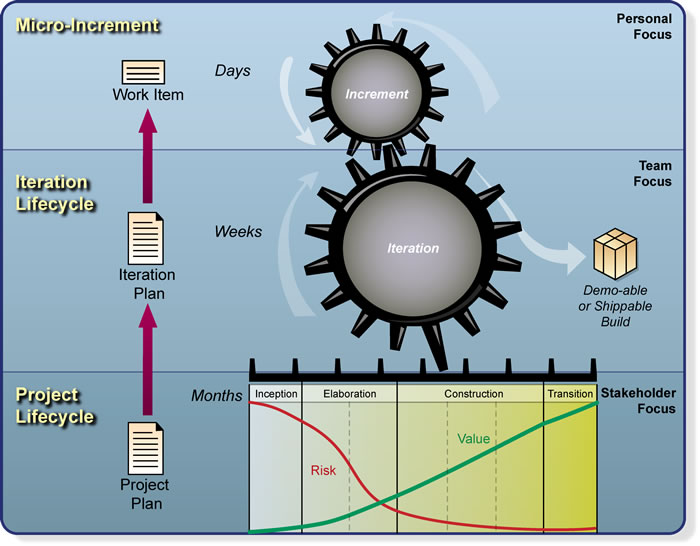
\includegraphics[width=0.8\linewidth]{3_openup}
	\caption[OpenUP lifecycle]{OpenUP lifecycle layers (source: \url{https://www.ida.liu.se/~TDDD77/openup/index.htm})}
	\label{fig:openUP}
\end{figure}

\begin{itemize}
\item The personal effort of an OpenUP project is defined as a \textbf{micro-increment}, commonly measured in hours or days.

\item From the team’s perspective, an \textbf{iteration lifecycle} reflects how micro-increments are applied to obtain stable and cohesive builds of the system being produced.

\item Focusing on how an overview of the project is guaranteed for the stakeholders, OpenUP structures the \textbf{project lifecycle} into four phases: \emph{Inception}, \emph{Elaboration}, \emph{Construction}, and \emph{Transition}.
\end{itemize}

%%%%%%%%%%%%%%%%%%%%%%%%%%%%%%%%%%%5

Thus, each of the phases of the OpenUP lifecycle are defined as follows:

\begin{itemize}

\item \textbf{Inception phase}: in this phase, it is a question of understanding what is intended to be produced and what are the objectives and limitations of the system to be developed, identifying the stakeholders, and detailing their success criteria.

\item \textbf{Elaboration phase}: it involves the procurement of a more detailed understanding of the system requirements; design, implementation, validation and establishment of the architecture baseline, providing a skeleton of the system structure; mitigation of essential risks and project planning in terms of time and costs.

\item \textbf{Construction phase}: iterative development of the desired product, until a tested result is achieved and ready to be offered to users. The goal pursued during this phase is to minimize costs through resource optimization and parallelization of independent tasks.

\item \textbf{Transition phase}: this last phase involves validating user expectancies, obtaining stakeholders approval, and seeking to improve future projects based on well-documented lessons learned.

\end{itemize}

These phases, applied to the particular case of this project, are presented in the following way:

\subsection{Inception phase}
\label{sec:inceptionPhase}

In this phase, the justification of the project was carried out, identifying its scope and the objectives to be pursued. Its feasibility in terms of risks, time and estimated costs was also assessed. Roles were assigned and, at the same time, an attempt was made at identifying the key functionalities of the system in accordance with the specifications defined with the identified stakeholders.

At this stage, the first meetings were held to establish the key functionalities of the system, to understand the competencies addressed and to provide an insight into how to proceed in the months ahead.

\subsection{Elaboration phase}
\label{sec:elaborationPhase}

Once an overview of the project had been established, a more detailed understanding of the objectives pursued was sought in this phase. To perform this task, a series of interviews with the stakeholders were planned and conducted, allowing to know the essential features that the system should meet. On this basis, the elicitation and formalised documentation of the system's requirements was carried out, allowing to proceed with the analysis and design of the functional modules that would compose the system.

Other tasks inherent to this stage were addressed, such as the choice of technological resources to be used, the development process employed, the definition of the system architecture baseline or the acquisition of domain-specific knowledge. Actors and use cases were also formally defined.

Finally, considering the set of formally stated requirements as well as the resulting skeleton of the system to be developed, a project planning consisting of time and cost estimation was elaborated. Based on the identified functionalities, the iterations that constitute the lifecycle were organized according to the priorities expressed by the stakeholders.

\subsection{Construction phase}
\label{sec:constructionPhase}

In this stage, the implementation of the different functionalities of the system was carried out. This implementation was undertaken in an orderly manner based on the preferences agreed upon with the stakeholders in the previous phase.

Presented in the order in which they were addressed, the following system functionalities were developed:

\begin{itemize}
\item \textbf{Module 1}: API skeleton. 
\item \textbf{Module 2}: Main user interface.
\item \textbf{Module 3}: STC measurement.
\item \textbf{Module 4}: Data visualization.
\item \textbf{Module 5}: Recommendation system.
\item \textbf{Module 6}: Settings and preferences.
\end{itemize}

The implementation of each module was done in an iterative way, trying to agree with the stakeholders (the project tutors) any kind of modification in the functionality or the interface considered during this development stage. As would be reflected in the planning, each functional module was associated with an iteration during the construction phase of the project.

\subsection{Transition phase}
\label{sec:transitionPhase}

Finally, the transition stage was dedicated to the documentation, testing and deployment of the system, confirming compliance with the requirements with the stakeholders and elaborating the final project report.

The review of the project by the tutors as well as the preparation of the project presentation were also part of this stage.

\section{Roles}
\label{sec:roles}

In this subsection, the set of basic OpenUP roles will be defined as well as the assignment of those roles for the concrete case of this project.

\begin{itemize}
\item \textbf{Analyst}: is the person in charge of identifying and understanding the problems and opportunities of the project, by knowing and interpreting the requirements expressed by the customer and end-users.

\item \textbf{Architect}: designs and documents the system architecture, being responsible for technical decisions on the overall implementation of the system.

\item \textbf{Developer}: each person in this role is responsible for the implementation of a set of parts of the system, adjusting it to the architecture and using the necessary technologies for the development.

\item \textbf{Project manager}: is the person in charge of planning the project, fulfilling the objectives as well as communicating and coordinating with the stakeholders.

\item \textbf{Tester}: person in charge of the identification, definition, implementation and execution of the tests over the system.

\item \textbf{Stakeholders}: people that may be directly or indirectly affected by project realization. Normally a stakeholder is a person whose needs will be met after the project is completed, like end-users o customers.
\end{itemize}

The general assignment of the OpenUP roles for this project is detailed in Table~\ref{tb:roles}.

\begin{table}[htb]
	\centering
	\caption[Roles assignment]{Roles assignment}
	\label{tb:roles}
	\begin{tabular}{|c|c|c|}
	\hline
	\textbf{Role}   & \textbf{Person}                           & \textbf{Charge}                  \\ \hline\hline
	Analyst         & \multirow{5}{*}{Antonio Manjavacas Lucas} & \multirow{5}{*}{Grade student}   \\ \cline{1-1}
	Architect       &                                           &                                  \\ \cline{1-1}
	Developer       &                                           &                                  \\ \cline{1-1}
	Project manager &                                           &                                  \\ \cline{1-1}
	Tester          &                                           &                                  \\ \hline
	Stakeholder     & Aurora Vizcaíno Barceló                   & Project supervisor and professor \\ \hline
	Stakeholder     & José Ángel Olivas Varela                  & Project supervisor and professor \\ \hline
	\end{tabular}
\end{table}


On the one hand, Aurora Vizcaíno was in charge of monitoring and providing feedback on the project: due to her experience in the field of GSD, she elicited the key requirements of the system, served as a guide throughout its planning and development and acted as a contact person for any queries during the project.

On the other hand, José Ángel Olivas was responsible for recommending and guiding the implementation of the modules related to the competencies of the Computing intensification, such as the underlying fuzzy logic mechanisms used to describe the communications and coordination between users by the expert system.

Finally, the tasks of analysis, design, development, testing, and documentation were carried out by Antonio Manjavacas, the grade student responsible for the project.

\section{Resources}
\label{sec:resources}

The following sub-sections will detail the hardware and software resources used in the development of this project.

\subsection{Hardware resources}
\label{sec:hardwareRes}

The hardware resources used are shown below:

\begin{itemize}
\item \href{https://www8.hp.com/}{HP} Pavilion x360 Convertible 14-cd0xxx equipped with:
	\begin{itemize}
	\item Intel(R) Core(TM) i7-8550U CPU @ 1.80GHz 1.99GHz, 64 bits
	\item 12 GB RAM
	\item Integrated graphics Intel(R) UHD Graphics 620
	\item NVIDIA GeForce MX130
	\end{itemize}
\end{itemize}

\subsection{Software resources}
\label{sec:softwareRes}

Likewise, these were the technologies, environments and programming languages used throughout the project:

\begin{itemize}

\item \href{https://www.java.com/}{Java 1.8}. General purpose, high level, object-oriented programming language. It is one of the most widely used programming languages by the developers community nowadays. Java stands out for its ease of learning and use, as well as its security and portability to any device capable of running Java Virtual Machine (JVM).\newline

\item \href{https://maven.apache.org/}{Apache Maven}. Tool for the management and automation of Java projects, facilitating dependencies management and software building. It is maintained by the Apache Software Foundation and is widely used by the Java community.\newline

\item \href{https://git-scm.com/}{Git}. Distributed version control system based on repositories. Facilitates version, branch, and data integrity management in software projects.\newline

\item \href{https://github.com/}{GitHub}. Hosting system for version control using Git. It facilitates the management of repositories and projects, offering multiple facilities in their creation and maintenance.\newline
	
\item \href{https://spring.io/}{Spring Framework}. Framework for the development of Java applications developed by Pivotal Software. It provides easy integration with Maven and other services to achieve the development of web applications.\newline

\item \href{https://www.mongodb.com/}{MongoDB}. Database management system, NoSQL and document based. Chosen for its easy use and optimization for the treatment of large data sets. Provides an easy integration with the rest of the tools employed, such as Spring framework.\newline
	
\item \href{https://www.mongodb.com/cloud/atlas/}{MongoDB Atlas}. MongoDB cloud database hosting service. It offers limited free storage as well as an easy connection and usage by applications via URI.\newline

\item \href{https://www.eclipse.org/ide/}{Eclipse}. Integrated Development Environment (IDE) widely used in Java development, among other languages. 
It includes utility plugins that facilitate integration with Git (\href{https://www.eclipse.org/egit/}{EGit}) or Maven (\href{https://www.eclipse.org/m2e/}{m2Eclipse}).\newline

\item \href{https://code.visualstudio.com/}{Visual Studio Code}. Free and open source code editor, which offers a large number of plugins and language support.\newline

\item \href{https://www.python.org/}{Python}. Interpreted, multi-paradigm, dynamic and multi-platform programming language. It stands out for its readability and usability.\newline

\item \href{http://jfuzzylogic.sourceforge.net/html/index.html}{jFuzzyLogic}. Java library for handling and working with fuzzy logic \cite{cingolani_jfuzzylogic_2012,cingolani_jfuzzylogic_2013}. It is based on the standard FCL (Fuzzy Control Language) and is freely distributed.\newline

\item \href{http://ffll.sourceforge.net/fcl.htm}{FCL}. Fuzzy Control Language published by the International Electrotechnical Commission (IEC). It is specified in the IEC 61131-7 document and allows the standardization of fuzzy control systems.\newline

\item \href{https://www.w3.org/html/logo/}{HTML 5}. Markup language used in web development. It is a standard in charge of the World Wide Web Consortium (W3C) and is currently in its version 5.\newline

\item \href{https://www.w3.org/Style/CSS/Overview.en.html}{CSS}. These cascading style sheets constitute a graphic design language used in conjunction with markup languages such as HTML. Used to enhance the appearance of user interfaces and customize their appearance.\newline
	
\item \href{https://getbootstrap.com/}{Bootstrap}. Open source multi-platform library for frontend design. It offers design templates based on HTML, CSS, and JavaScript.\newline

\item \href{https://www.javascript.com/}{JavaScript}. Interpreted, object-oriented, prototype-based, imperative, weakly typed and dynamic programming language. Widely used in client-side web development.\newline

\item \href{https://www.chartjs.org/}{Chart.js}. Open source JavaScript library for creating graphics and animations in HTML5.\newline

\item \href{https://jquery.com/}{jQuery}. JavaScript library aimed to simplify interaction with HTML and make client-side AJAX  (Asynchronous JavaScript And XML) requests in web applications.\newline

\item \href{https://www.postman.com/}{Postman}. A tool for the creation of API requests in a simple and fast way. It eases the testing of web applications and allows a high customization of the requests.\newline

\item \href{https://www.heroku.com/}{Heroku}. Cloud Computing Platform as a Service (PaaS). Enables deployment of cloud applications and offers limited free hosting.\newline

\item \href{https://ubuntu.com/}{Ubuntu}. Free and open-source Linux distribution distributed by Canonical Ltd. Used in the deployment procedure and part of the application development.\newline

\item \href{https://www.microsoft.com/en-us/windows/}{Windows 10}. Operating system developed and distributed by Microsoft. Used in most of the application development.\newline

\item \href{https://www.zotero.org/}{Zotero}. Free and open bibliographic reference manager. It is multi-platform and offers a browser extension that facilitates the management and collection of references.\newline

\item \href{https://www.latex-project.org/}{\LaTeX}. Markup language oriented to the elaboration and layout of high-quality documents. Based on \TeX, initially developed by Donald Knuth. The template available in \cite{salidoTFGgit} has been used to elaborate this document.\newline
	
\item \href{https://www.texstudio.org/}{{\TeX}studio}. Integrated writing IDE for creating \LaTeX documents. {\TeX}studio is open source and available for all major operating systems.\newline

\item \href{https://www.microsoft.com/en-us/microsoft-365/word/}{Microsoft Word}. WYSIWYG text editor distributed by Microsoft in its Microsoft Office package. Used for the elaboration of the draft memory and basic documental tasks during the project.\newline

\item \href{https://www.microsoft.com/en-us/microsoft-365/onedrive/online-cloud-storage/}{Microsoft OneDrive}. Cloud data storage system offered by Microsoft. Used for the storage of documents, backups, code, and diagrams.\newline

\item \href{https://www.diagrams.net/}{Diagrams.net}. Previously known as Draw.io, it is a tool for creating diagrams and charts. It is open source and offers online and desktop support.\newline

\end{itemize}

Finally, a summary of the software resources used is shown in Figure~\ref{fig:swResources}.

\begin{figure}[htb]
	\centering
	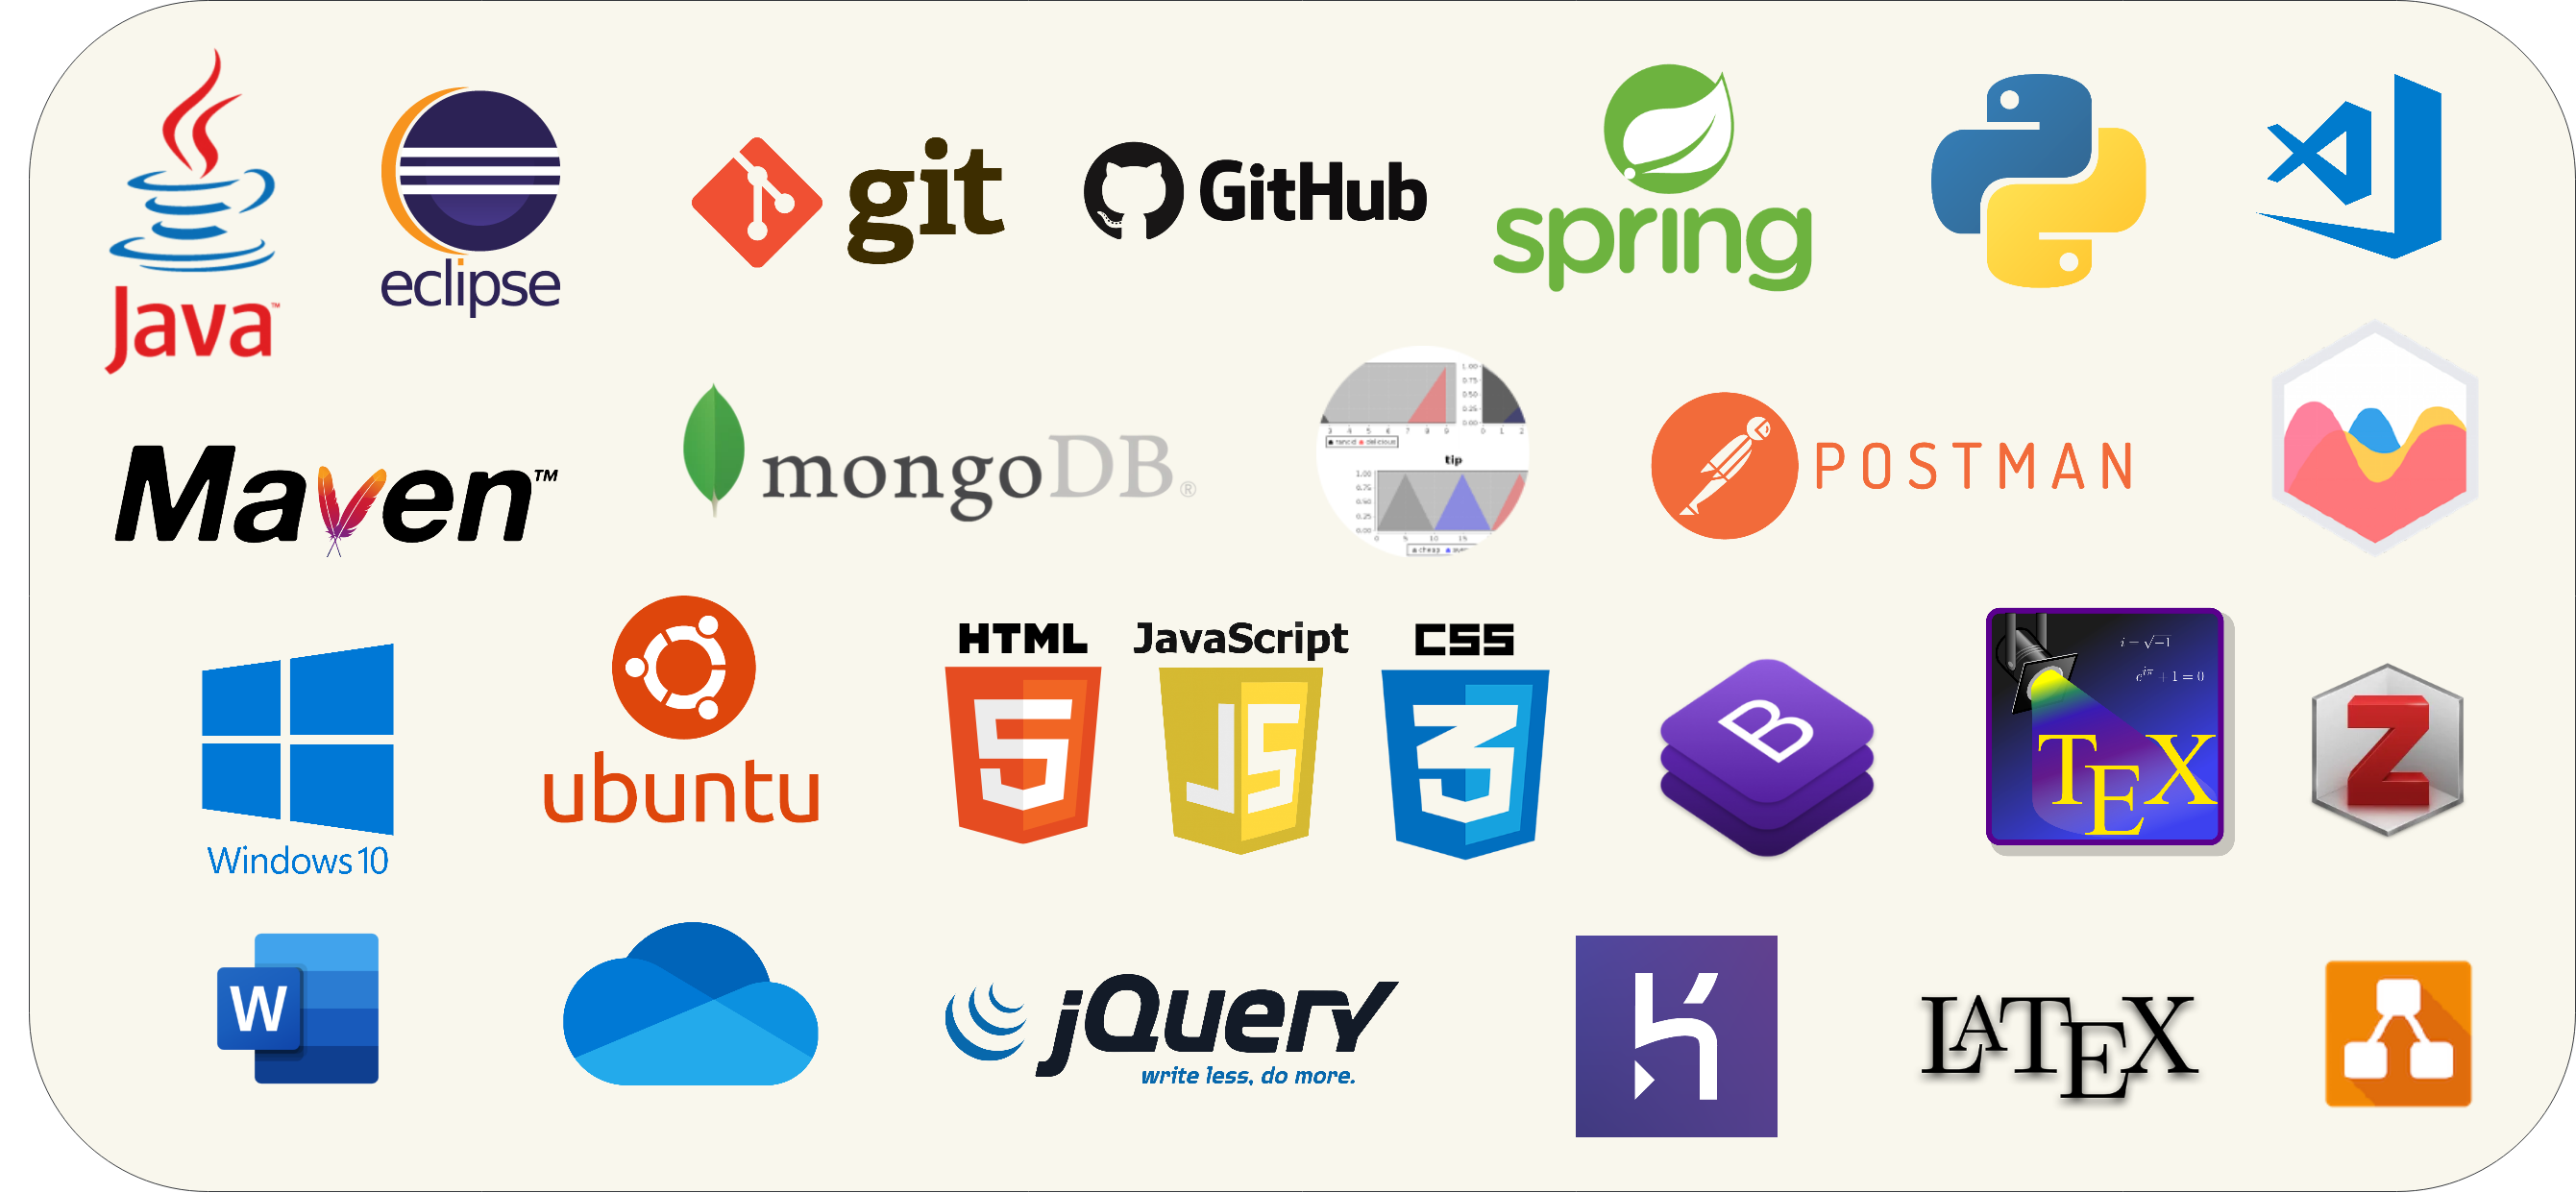
\includegraphics[width=0.9\linewidth]{3_tools}
	\caption[Software resources]{Software resources used in this project}
	\label{fig:swResources}
\end{figure}



\chapter{Results}
\label{cap:results}

In accordance with the OpenUP lifecycle described in chaper~\ref{cap:methodology}, the following subsections will detail the development phases of the first version of FENCE, emphasizing the results of each phase and thoroughly explaining the decisions made in the design and development of the tool.

\section{Inception phase}

In this first phase, initial meetings with stakeholders took place, where a first contact was established and from which the project objectives would begin to be defined. The idea of the preliminary project was consolidated, and the functionalities and design of FENCE began to be roughly sketched out.

Therefore, this meetings with the stakeholders, Aurora Vizcaíno and José Ángel Olivas, focused on defining, on the one hand, the basic functionalities of the tool (STC measurement, dashboard features, settings and preferences) and, on the other hand, the features that would make FENCE an innovative tool (use of fuzzy control system to improve STC measurement or a recommending system aimed to enhance STC levels). These features were conveniently formalized as requirements, as we will see in the elaboration phase.

As previously mentioned, the initiation phase in OpenUP involves the definition of the roles of the different stakeholders. In this case, it was decided that Aurora Vizcaíno would supervise the development of the application in general terms, while José Ángel Olivas would monitor the part of the system related to the intensification competencies, such as the implementation of the expert system or the introduction of fuzzy logic into the system.

Moreover, from a technical point of view, it was also agreed that FENCE would be a web application capable of offering services locally and, if possible, online. Furthermore, ideas also began to be sketched out on what the web application would graphically look like, as shown in the sketches represented in Figure~\ref{fig:dash_mockup} and Figure~\ref{fig:rec_mockup}.

\begin{figure}
	\centering
	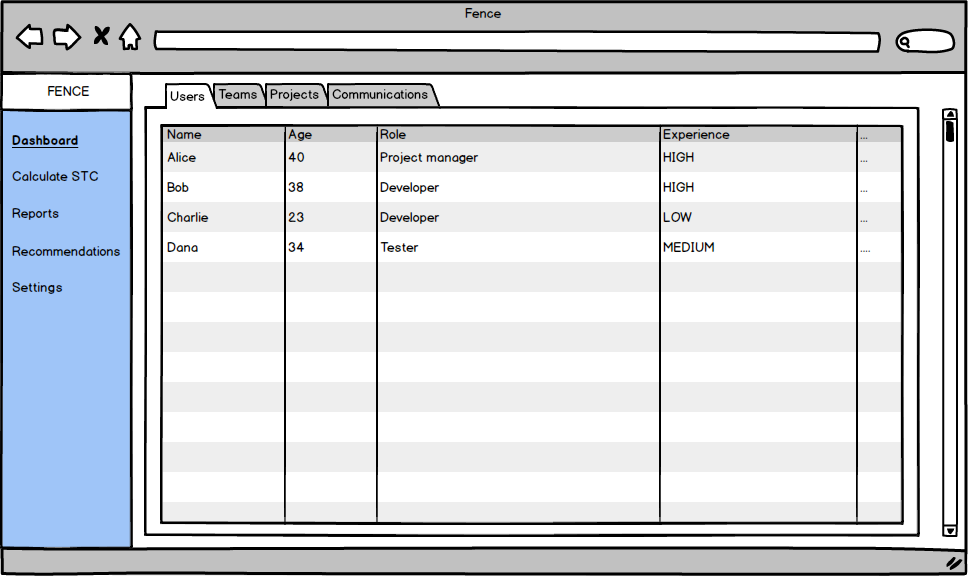
\includegraphics[width=0.9\linewidth]{4_mockup-dashboard}
	\caption[Dashboard mockup]{Dashboard mockup}
	\label{fig:dash_mockup}
\end{figure}

\begin{figure}
	\centering
	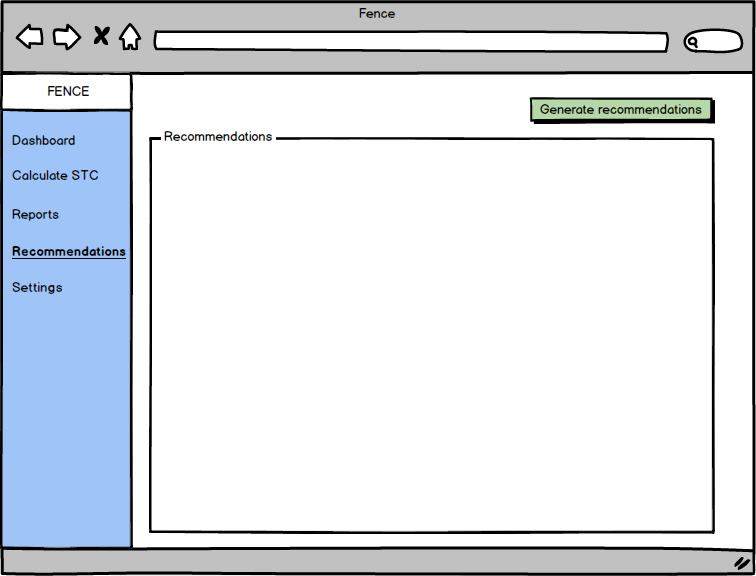
\includegraphics[width=0.9\linewidth]{4_mockup-recommendations}
	\caption[Recommendations window mockup]{Recommendations window mockup}
	\label{fig:rec_mockup}
\end{figure}

With clear objectives and an approximate and viable idea of the project to be undertaken, we proceeded to the elaboration phase, where these objectives and requirements would be formalized thus establishing the foundations of FENCE.

\section{Elaboration phase}

Initially, the objectives pursued in this phase are the formalization of the system requirements, the decision on the architecture to be used, as well as its design and data model. On this basis, it would be possible to establish a project planning, as well as a cost estimate adjusted to the development time and resources used.

Moreover, some key learning aspects were carried out at this stage, such as training in the Spring framework or MongoDB. Thus, further research in these technologies in the early project stages would facilitate future work and ensure more consistent progress.

\subsection{Requirements}

The requirements elicitation is the process in which the description of the properties that the system to be developed must meet is performed. These features are expressed by the client, while the interviewer is in charge of collecting the necessary information and expressing it in a precise and unambiguous document.

In the case of this project, the process of requirements elicitation was carried out following the structured interview method, as detailed in \cite{toro_metodologia_2000}. These interviews are divided in three phases: preparation, realization and analysis, and they are a close and direct way to directly understand interests of the stakeholders. Therefore, the interview was approached as follows:

\begin{itemize}
	\item First the questions to be asked were decided, a structured script was drawn up with the questions to be asked and the order to be followed.
	\item Subsequently, a first meeting was held with the main stakeholder, Aurora Vizcaíno, where the functional and non-functional requirements of the tool were broadly agreed upon.
	\item Regular follow-up meetings would be held throughout the project, where these requirements would be not only evaluated but also adjusted to suggested changes and improvements.
\end{itemize}

The initial requirements were expressed in precise and unambiguous language, as will be shown in the following subsections. Thus, after their validation by the client, the use cases and modelling of FENCE would proceed.

\subsubsection{FUNCTIONAL REQUIREMENTS}

Functional requirements represent which functionalities should be covered by the system to be developed, considering inputs and outputs as well as the behaviour of the software. After the interviews with stakeholders, these functional requirements were agreed upon and duly expressed, giving rise to the set of functionalities represented in Table~\ref{tb:funct-req}.

\begin{table}
	\centering
	\caption[Functional requirements]{Functional requirements}
	\label{tb:funct-req}
	\resizebox{\textwidth}{!}{%
	\begin{tabular}{|c|c|l|c|}
	\hline
	\textbf{ID} &
	  \textbf{Description} &
	  \multicolumn{1}{c|}{\textbf{Objectives}} &
	  \textbf{Priority} \\ \hline\hline
	\textit{FR1} &
	  Users STC measurement &
	  \begin{tabular}[c]{@{}l@{}}The tool must calculate and display  the STC \\ levels of the users in the organization.\end{tabular} &
	  High \\ \hline
	\textit{FR2} &
	  Teams STC measurement &
	  \begin{tabular}[c]{@{}l@{}}The tool must calculate and display the STC \\ levels of the teams in the organization.\end{tabular} &
	  High \\ \hline
	\textit{FR3} &
	  Projects STC measurement &
	  \begin{tabular}[c]{@{}l@{}}The tool must calculate the STC \\ levels of the projects in the organization.\end{tabular} &
	  High \\ \hline
	\textit{FR4} &
	  Recommendations &
	  \begin{tabular}[c]{@{}l@{}}The system must provide recommendations \\ based on the existing coordination gaps to improve \\ the STC levels of the organization.\end{tabular} &
	  High \\ \hline
	\textit{FR5} &
	  Dashboard: employees &
	  \begin{tabular}[c]{@{}l@{}}The tool should allow to perform CRUD \\ operations over employees as resources.\end{tabular} &
	  Medium \\ \hline
	\textit{FR6} &
	  Dashboard: teams &
	  \begin{tabular}[c]{@{}l@{}}The tool should allow to perform CRUD\\ operations over teams as resources.\end{tabular} &
	  Medium \\ \hline
	\textit{FR7} &
	  Dashboard: projects &
	  \begin{tabular}[c]{@{}l@{}}The tool should allow to perform CRUD \\ operations over  projects as resources.\end{tabular} &
	  Medium \\ \hline
	\textit{FR8} &
	  Dashboard: tasks &
	  \begin{tabular}[c]{@{}l@{}}The tool should allow to perform CRUD \\ operations over tasks as resources.\end{tabular} &
	  Medium \\ \hline
	\textit{FR9} &
	  Dashboard: task assignments &
	  \begin{tabular}[c]{@{}l@{}}The tool should allow to perform CRUD \\ operations over tasks assignments as resources.\end{tabular} &
	  Medium \\ \hline
	\textit{FR10} &
	  Dashboard: task dependencies &
	  \begin{tabular}[c]{@{}l@{}}The tool should allow to perform CRUD \\ operations over tasks dependencies as resources.\end{tabular} &
	  Medium \\ \hline
	\textit{FR11} &
	  Dashboards: communications &
	  \begin{tabular}[c]{@{}l@{}}The tool should allow to visualize \\ communications within the organization.\end{tabular} &
	  Medium \\ \hline
	\textit{FR12} &
	  Users STC visualization &
	  \begin{tabular}[c]{@{}l@{}}The tool should display visual information \\ about the users' STC levels along time.\end{tabular} &
	  Low \\ \hline
	\textit{FR13} &
	  Teams STC visualization &
	  \begin{tabular}[c]{@{}l@{}}The tool should display visual information \\ about the teams’ STC levels along time.\end{tabular} &
	  Low \\ \hline
	\textit{FR14} &
	  Projects STC visualization &
	  \begin{tabular}[c]{@{}l@{}}The tool should display visual information \\ about the projects' STC levels along time.\end{tabular} &
	  Low \\ \hline
	\textit{FR15} &
	  Custom project‘s lack of coordination threshold &
	  \begin{tabular}[c]{@{}l@{}}The tool will allow to customize from which \\ threshold of lack of coordination recommendations \\ should be provided for a given project.\end{tabular} &
	  Low \\ \hline
	\textit{FR16} &
	  Custom users’ lack of coordination threshold &
	  \begin{tabular}[c]{@{}l@{}}The tool will allow to customize from which \\ threshold of lack of coordination recommendations \\ should be provided for a given pair of employees \\ within a project.\end{tabular} &
	  Low \\ \hline
	\end{tabular}%
	}
\end{table}

\subsubsection{NON FUNCTIONAL REQUIREMENTS}

Non-functional requirements are complemented by functional requirements to fully define the expected characteristics of the system. These requirements focus on representing quality and technical features as well as conditions and constraints expressed by the customer. Thus, the non-functional requirements for this project are shown in the Table~\ref{tb:nonfunc-req}.

\begin{table}
	\centering
	\caption{Non-functional requirements}
	\label{tb:nonfunc-req}
	\resizebox{\textwidth}{!}{%
	\begin{tabular}{|c|c|l|c|}
	\hline
	\textbf{ID} &
	  \textbf{Description} &
	  \multicolumn{1}{c|}{\textbf{Objectives}} &
	  \textbf{Type} \\ \hline\hline
	\textit{NFR1} &
	  Labels &
	  \begin{tabular}[c]{@{}l@{}}Linguistic labels will be used to represent ambiguous terms,   \\ such as user experience, English level, or dependency weight \\ between tasks.\end{tabular} &
	  Usability \\ \hline
	\textit{NFR2} &
	  Web application &
	  \begin{tabular}[c]{@{}l@{}}The application will be deployed as a web service, preferably  \\  at a local level, but with the possibility of public offering.\end{tabular} &
	  Usability \\ \hline
	\textit{NFR3} &
	  Browser compatibility &
	  \begin{tabular}[c]{@{}l@{}}The application must be able to run on desktop devices using   \\ conventional browsers such as Google Chrome or Mozilla Firefox.\end{tabular} &
	  Compatibility \\ \hline
	\textit{NFR4} &
	  Cloud database &
	  \begin{tabular}[c]{@{}l@{}}A database management system available in the cloud will be   \\ used, in order to facilitate the integration of the tool with remote systems.\end{tabular} &
	  Compatibility \\ \hline
	\textit{NFR5} &
	  Performance &
	  \begin{tabular}[c]{@{}l@{}}The application will run fluently in the interaction with   \\ its different components, offering an adequate performance and user  \\  experience.\end{tabular} &
	  Performance \\ \hline
	\end{tabular}%
	}
\end{table}

\subsection{Use cases and modules}

Once the system requirements had been compiled, the definition of the use cases was undertaken. The use case model is shown in Figure~\ref{fig:cdu-model}, which represents the activities carried out by the entities (actors) according to the expected system functionalities.

\begin{figure}
	\centering
	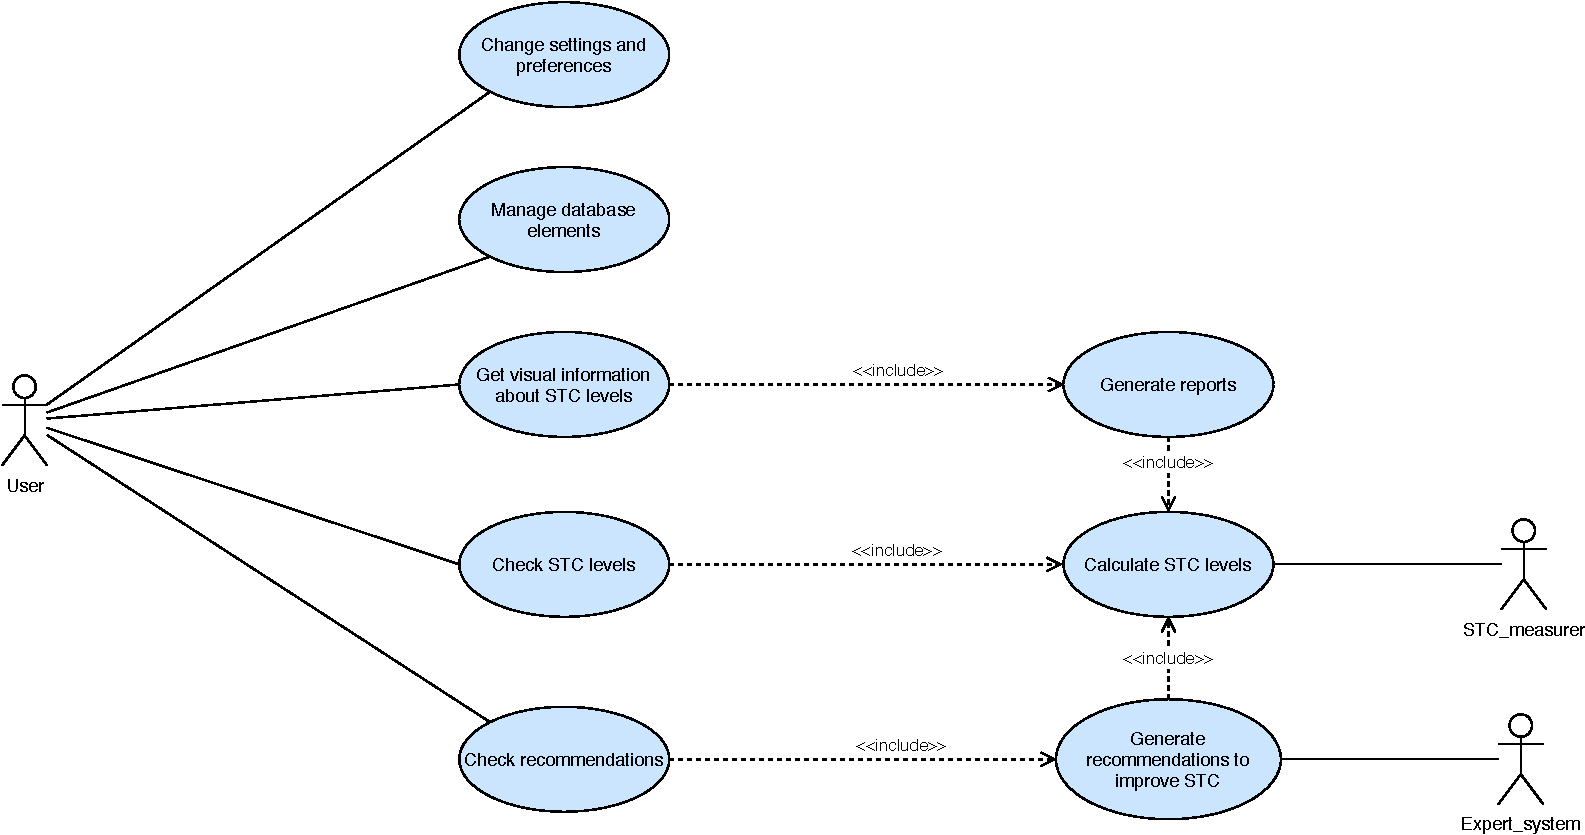
\includegraphics[width=0.95\linewidth]{4_cdu-diagram}
	\caption[Use cases model]{Use cases model}
	\label{fig:cdu-model}
\end{figure}

Once the use cases were identified, they were grouped into different functional modules in order to organize the development of the subsystems that compose the application. These are listed in Table~\ref{tb:func-mod}, together with their definitions and priority levels.

\begin{table}
	\centering
	\caption{Functional modules}
	\label{tb:func-mod}
	\resizebox{\textwidth}{!}{%
	\begin{tabular}{|c|c|l|c|}
	\hline
	\textbf{ID} &
	  \textbf{Module description} &
	  \multicolumn{1}{c|}{\textbf{Objectives}} &
	  \textbf{Priority} \\ \hline\hline
	\textit{M1} &
	  API skeleton &
	  \begin{tabular}[c]{@{}l@{}}Development of the application skeleton, creation of the API   \\ resources as well as connection and operations on the database.\end{tabular} &
	  High \\ \hline
	\textit{M2} &
	  Main  user interface &
	  \begin{tabular}[c]{@{}l@{}}Implementation of the dashboard functionalities and   \\ elaboration of the main windows of the web application.\end{tabular} &
	  High \\ \hline
	\textit{M3} &
	  STC measurement &
	  \begin{tabular}[c]{@{}l@{}}Extraction of assignments, dependencies, and current   \\ coordination, as well as coordination requirements and gaps. \\ Computation of STC at employees, teams, and projects levels.\end{tabular} &
	  High \\ \hline
	\textit{M4} &
	  Data visualization &
	  \begin{tabular}[c]{@{}l@{}}Graphic representation of the STC levels history, allowing   \\ to see comparisons and the variation of these levels along time.\end{tabular} &
	  Medium \\ \hline
	\textit{M5} &
	  Recommendation system &
	  \begin{tabular}[c]{@{}l@{}}System for the detection of coordination gaps and   \\ recommendation of solutions to improve the levels \\ of STC based on expert knowledge.\end{tabular} &
	  Medium \\ \hline
	\textit{M6} &
	  Settings and preferences &
	  Customization and tool settings configuration. &
	  Low \\ \hline
	\end{tabular}%
	}
\end{table}

The decomposition of the application in functional modules would facilitate the way to proceed in the construction phase of the life cycle, performing micro-increments that could be tested and evaluated by the stakeholders. This modular division would also facilitate the planning and estimation of development times, as it will be seen in the following sub-section.

\subsection{Planification}

Having identified the functionalities to be implemented and the general project decomposition, it was divided into the iterations shown in Table~\ref{tb:proj-iters}. Each one, with an estimated duration, would represent an evaluable and revisable micro-increment of the application.

\begin{table}
	\centering
	\caption{Project iterations}
	\label{tb:proj-iters}
	\begin{tabular}{|c|l|c|}
	\hline
	\textbf{Iteration} &
	  \multicolumn{1}{c|}{\textbf{Summary}} &
	  \textbf{Estimated time} \\ \hline\hline
	\textit{IT0} &
	  \begin{tabular}[c]{@{}l@{}}Definition of general objectives, first draft and   \\ preliminary meetings.\end{tabular} &
	  1 week \\ \hline
	\textit{IT1} &
	  \begin{tabular}[c]{@{}l@{}}Planning, requirements elicitation, role assignment, \\ usecase modelling and design.\end{tabular} &
	  2 weeks \\ \hline
	\textit{IT2} & Module 1 implementation             & 1 week  \\ \hline
	\textit{IT3} & Module 2 implementation             & 2 weeks \\ \hline
	\textit{IT4} & Module 3 implementation             & 4 weeks \\ \hline
	\textit{IT5} & Module 4 implementation             & 1 week  \\ \hline
	\textit{IT6} & Module 5 implementation             & 3 weeks \\ \hline
	\textit{IT7} & Module 6 implementation             & 1 week  \\ \hline
	\textit{IT8} & Documentation, tests and deployment & 3 weeks \\ \hline
	\textit{IT9} & Review and submission preparation   & 2 weeks \\ \hline
	\end{tabular}
\end{table}

Based on these iterations, the project schedule was established (see Table~\ref{tb:schedule}). This was largely achieved, apart from some slight fluctuations which did not affect the project, as they were due to improvements in the different functional modules, rather than delays.

\begin{table}
	\centering
	\caption{Project scheduling}
	\label{tb:schedule}
	\resizebox{\textwidth}{!}{%
	\begin{tabular}{|c|c|c|c|c|c|c|c|c|c|}
	\hline
	\textbf{Inception phase} &
	  \textbf{Elaboration phase} &
	  \multicolumn{6}{c|}{\textbf{Construction phase}} &
	  \multicolumn{2}{c|}{\textbf{Transition phase}} \\ \hline\hline
	\textit{IT0} &
	  \textit{IT1} &
	  \textit{IT2} &
	  \textit{IT3} &
	  \textit{IT4} &
	  \textit{IT5} &
	  \textit{IT6} &
	  \textit{IT7} &
	  \textit{IT8} &
	  \textit{IT9} \\ \hline
	\begin{tabular}[c]{@{}c@{}}From: 7th \\ January\\  -   \\ To: 31st\\  January\end{tabular} &
	  \begin{tabular}[c]{@{}c@{}}From: 1st \\ February\\ -  \\ To: 15th \\ February\end{tabular} &
	  \begin{tabular}[c]{@{}c@{}}From: 16th \\ February\\   -  \\    To: 23th \\ February\end{tabular} &
	  \begin{tabular}[c]{@{}c@{}}From: 24th\\  February\\   -  \\ To: 8th\\ March\end{tabular} &
	  \begin{tabular}[c]{@{}c@{}}From: 9th \\ March\\   -    \\ To: 5th\\ April\end{tabular} &
	  \begin{tabular}[c]{@{}c@{}}From: 6th \\ April\\   -  \\    To: 12th \\ April\end{tabular} &
	  \begin{tabular}[c]{@{}c@{}}From: 13th \\ April\\  -   \\    To: 3rd \\ May\end{tabular} &
	  \begin{tabular}[c]{@{}c@{}}From: 4th \\ May\\  -   \\    To: 10th \\ May\end{tabular} &
	  \begin{tabular}[c]{@{}c@{}}From: 11th \\ May\\   -  \\    To: 31st \\ May\end{tabular} &
	  \begin{tabular}[c]{@{}c@{}}From: 1st \\ June\\  -  \\    To: 14th \\ June\end{tabular} \\ \hline
	1 week &
	  2 weeks &
	  1 week &
	  2 weeks &
	  4 weeks &
	  1 week &
	  3 weeks &
	  1 week &
	  3 weeks &
	  2 weeks \\ \hline
	1 week &
	  2 weeks &
	  \multicolumn{6}{c|}{12 weeks} &
	  \multicolumn{2}{c|}{3 weeks} \\ \hline
	\multicolumn{10}{|c|}{\textbf{Total: 18 weeks}} \\ \hline
	\end{tabular}%
	}
\end{table}

\subsection{Cost estimation}

In this section, the cost estimation of the project, calculated from the working time and resources used, is broken down. For this estimation, the variables shown in Table~\ref{tb:costs} have been considered, giving rise to the total cost of 7206.6 €.

\begin{table}
	\centering
	\caption{Project cost estimation}
	\label{tb:costs}
	\begin{tabular}{c|c|}
	\hline
	\multicolumn{1}{|c|}{\textbf{Variable}}   & \textbf{Value}                      \\ \hline\hline
	\multicolumn{1}{|c|}{Total working hours} & $\approx$ 630 hours $*$ 11,22 €/hour = 7068 € \\ \hline
	\multicolumn{1}{|c|}{\begin{tabular}[c]{@{}c@{}}Indirect investments \\ (resources, electricity consume, etc.)\end{tabular}} & 138.6   € \\ \hline
	                                          & 7206.6   €                          \\ \cline{2-2} 
	\end{tabular}%
	
\end{table}

The salary per hour of the analyst-programmer is reflected in \cite{tecnoempleo}, with data updated up to May 2020. At the same time, the price of software resources has been omitted because only free software or software covered by academic licenses has been used.

\subsection{Architecture and design}

The elaboration phase of the OpenUp lifecycle includes the selection of the architecture to be employed. So, at this stage it was decided that FENCE would be a client-server application based on a layered architecture, whose characteristics are described below. The choice of client-server as the architecture of FENCE was agreed in order to be able to deploy the tool as a web service if necessary. In this way, this would be a portable application, which would allow the user to run the tool from any browser without the need for additional software.

Moreover, a preliminary data model was also established, establishing the main collections and documents that would comprise it, as well as their attributes and possible relationships.

\subsubsection{LAYERED ARCHITECTURE}

Layer-based architecture \cite{layered_architecture} is one of the most common design patterns in the development of client-server web applications. In this type of architecture, the different modules that comprise the system (layers) are organized horizontally, so that each layer of the application fulfils a specific role.

Spring Boot \cite{spring_boot} provides a great simplicity when implementing this type of RESTful layered services \cite{api_rest},  so it is on this basis on which the FENCE architecture is based (see Figure~\ref{fig:layer_arch} and Figure~\ref{fig:layers-sample}):

\begin{figure}
	\centering
	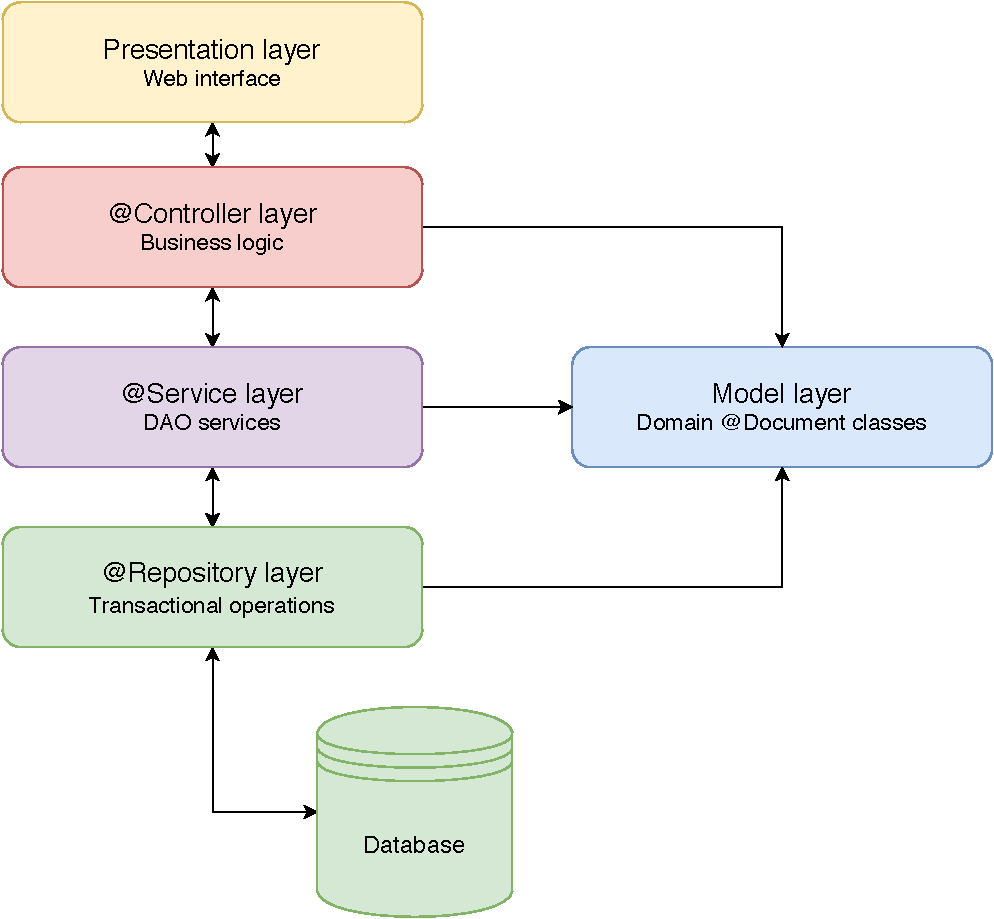
\includegraphics[width=0.8\linewidth]{4_layered-architecture}
	\caption[Layered architecture]{Layered architecture}
	\label{fig:layer_arch}
\end{figure}

\begin{figure}
	\centering
	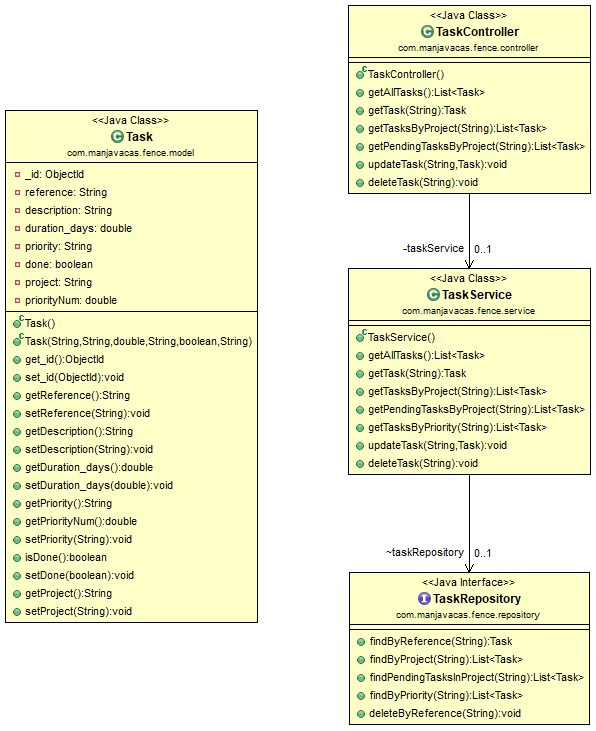
\includegraphics[width=0.65\linewidth]{4_sample-layers}
	\caption[Sample connection between layers]{Sample connection between layers}
	\label{fig:layers-sample}
\end{figure}

\begin{itemize}
\item \textbf{Presentation}. It is the layer in charge of the interaction with the user. In this case, it includes the static resources (HTML views and CSS code), as well as the underlying JavaScript code. This layer, conceived as the client side, communicates with the server through GET, POST, PUT or DELETE AJAX requests.
\item \textbf{Model}. This is the layer where the classes that model real-world entities are found. These classes, making use of the Spring framework integration with MongoDB, are labelled as documents (\textit{@Document}), so that they represent the basic structure of the documents included in the database's collections.
\item \textbf{Controller}. The controllers are the classes in charge of handling the CRUD requests received from the presentation layer. They make use of the classes defined in the Model layer, are labelled as \textit{@Controller}, and establish, for each of the CRUD operations, a mapping with their methods. In general, this layer covers business logic operations, so we can also find controller classes in charge of performing other transactions besides attending to requests from the presentation layer. Furthermore, when any of these operations requires access to the database, communication with the underlying DAO (Data Access Only) layers will be necessary.
\item \textbf{Service}. This layer includes the set of DAO classes that interact with the database. They are labelled as \textit{@Service} and include the logic needed to access repositories and handle controller requests.
\item \textbf{Repository}. Repository. MongoDB repositories are a type of interface included in Spring that provides easy and flexible interaction with MongoDB collections. They allow database queries to be abstracted and customized and are labelled as \textit{@Repository}. 
\end{itemize}

If we go deeper into the FENCE architecture at a class level, we will always find a similar pattern: the class controller attends to CRUD requests from the interface and, in case of requiring stored data, on request to the service class, the data is retrieved through the corresponding repository interface. This general procedure is summarized in Figure~\ref{fig:layer_int}.

\begin{figure}
	\centering
	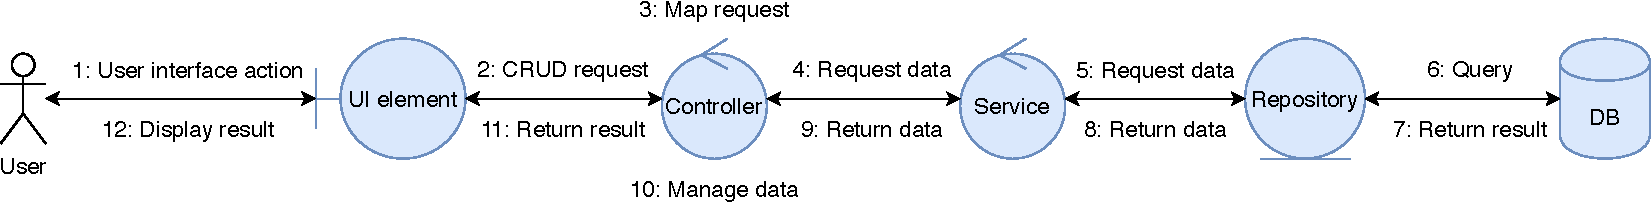
\includegraphics[width=0.95\linewidth]{4_layered-interaction}
	\caption[Layered interaction]{Layered interaction}
	\label{fig:layer_int}
\end{figure}

\subsubsection{DATA MODEL}

The reasons for using a noSQL database system like MongoDB are the advantages that this type of environments provide:

\begin{itemize}
\item On the one hand, they offer great flexibility during development, especially if we consider the easy integration of MongoDB with Spring framework.
\item On the other hand, the modification of noSQL schemes is very simple, fast, and scalable.
\item In addition, MongoDB databases also integrate SQL features and queries, so we can have the best of both types of databases in the same system.
\end{itemize}

However, although there are disadvantages when using noSQL, such as manual control of data consistency or operation atomicity, the data model of FENCE was not considered complex enough to make a SQL system more convenient.

As indicated, Spring's integration with MongoDB is relatively simple. We only need to label the classes we want to represent as database documents with \textit{@Document} in order to establish their schema. This will make it indexable through the \textit{@Repository} interfaces and easily accessible. An  of the correspondence between a class labelled as \textit{@Document} and its instance in the database is shown in Figure~\ref{fig:doc_sample}.

\begin{figure}
	\centering
	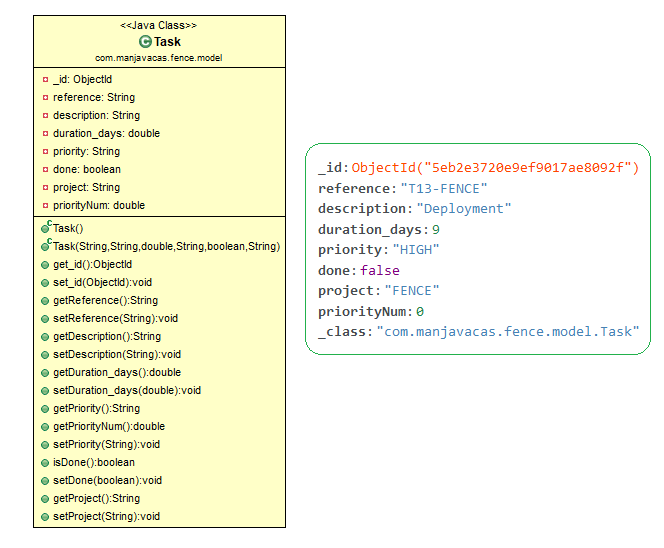
\includegraphics[width=0.65\linewidth]{4_sample-document}
	\caption[Relation between Java class and MongoDB document]{Relation between Java class and MongoDB document}
	\label{fig:doc_sample}
\end{figure}

On this basis, the scheme shown in Figure~\ref{fig:data_model} represents the data model of FENCE, where the \textit{@Document} classes and their relationships can be appreciated.

\begin{figure}
	\centering
	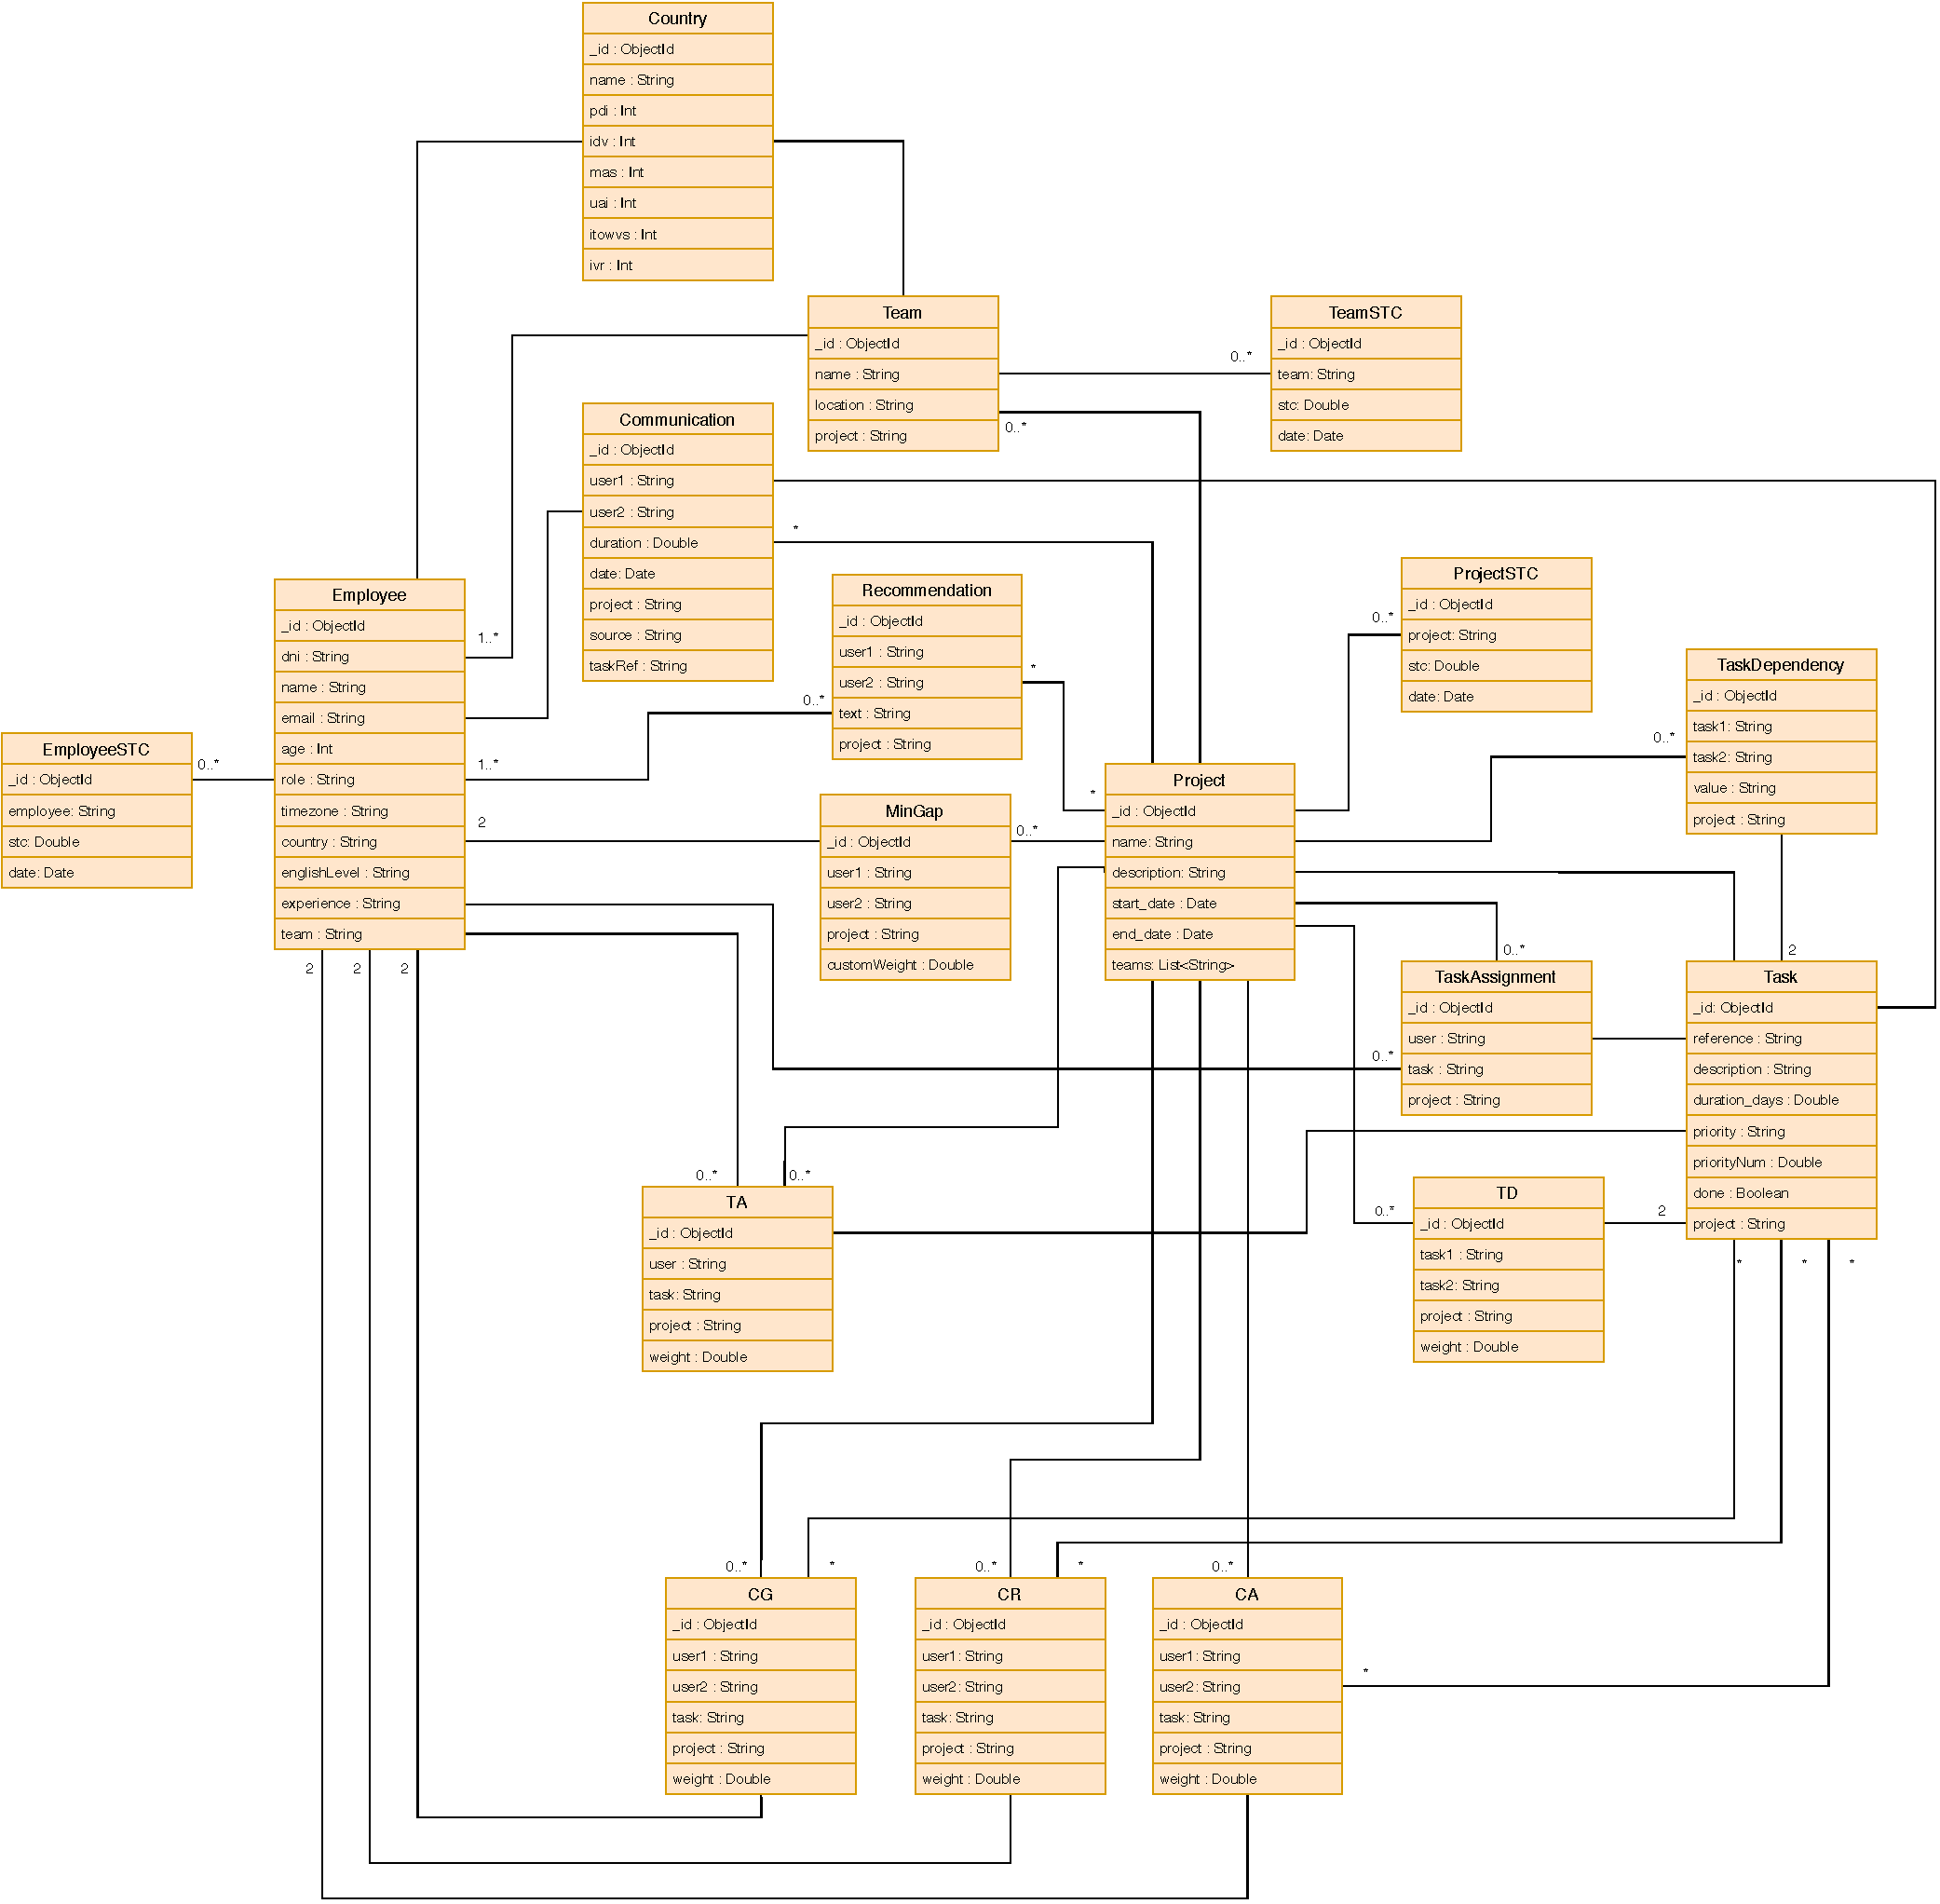
\includegraphics[width=0.95\linewidth]{4_data-model}
	\caption[FENCE data model]{FENCE data model}
	\label{fig:data_model}
\end{figure}

Therefore, once the architecture and data model of the system had been defined, the implementation of the different functional modules of FENCE was undertaken.

\section{Construction phase}

The following subsections will address in detail the process of developing the functionalities of FENCE, as well as the difficulties and decisions faced in its implementation. The implementation of each of these modules meant a micro-increment in the functionalities of FENCE, giving as a result the first version of the application.

\subsection{Module 1. API skeleton}

The first objective pursued in this phase was the creation of the initial set of resources that compose the application, as well as the main windows that would define the structure of the system's interface. Throughout this stage, the main structure of the data model was established, which would be progressively expanded throughout the project.

Thus, taking as a reference this initial data model and the previously designed class diagram, the different classes, URIs and query methods were defined. Likewise, as shown in Figure~\ref{fig:mongodb-cluster}, the MongoDB cluster hosted in the MongoDB Atlas cloud service was created, establishing access permissions, integrating the MongoDB Java Driver into the Maven project, and making queries operational through Spring.

\begin{figure}
	\centering
	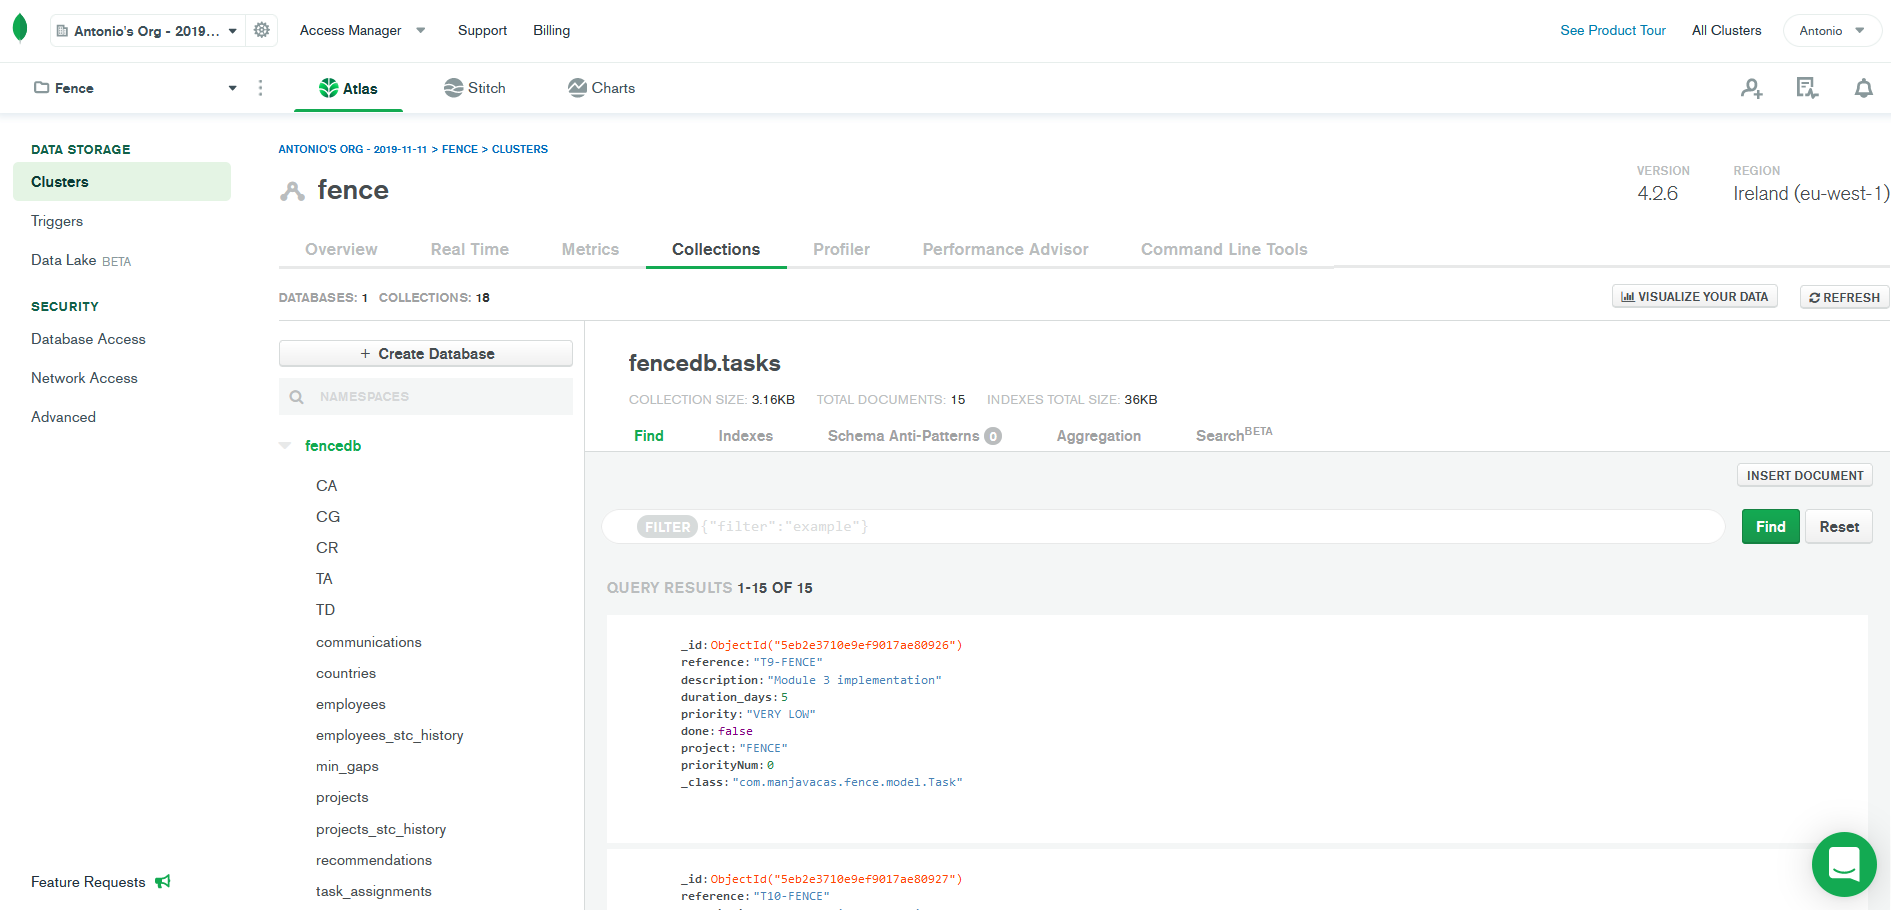
\includegraphics[width=0.95\linewidth]{4_mongodb-atlas}
	\caption[MongoDB Atlas cluster]{MongoDB Atlas cluster}
	\label{fig:mongodb-cluster}
\end{figure}

Once the cluster’s database was created and correctly integrated into the system, the main CRUD operations were added for each of the resources, defining the necessary methods in Controllers, Services and Repositories. Following the model provided by Spring framework, each application resource is represented by a class from the Model package, as previously explained. On the other hand, controllers are in charge of the main operations and communication with the interface, while service classes act as DAO entities communicating with the MongoDB repositories (as shown in Figure~\ref{fig:layer_arch}.

Therefore, when the logical skeleton of the application had been created, the two main windows of the system were elaborated. On the one hand, the main control panel that would be gradually completed in the different iterations of the project, whose first version is shown in Figure~\ref{fig:first-dashboard}.

\begin{figure}
	\centering
	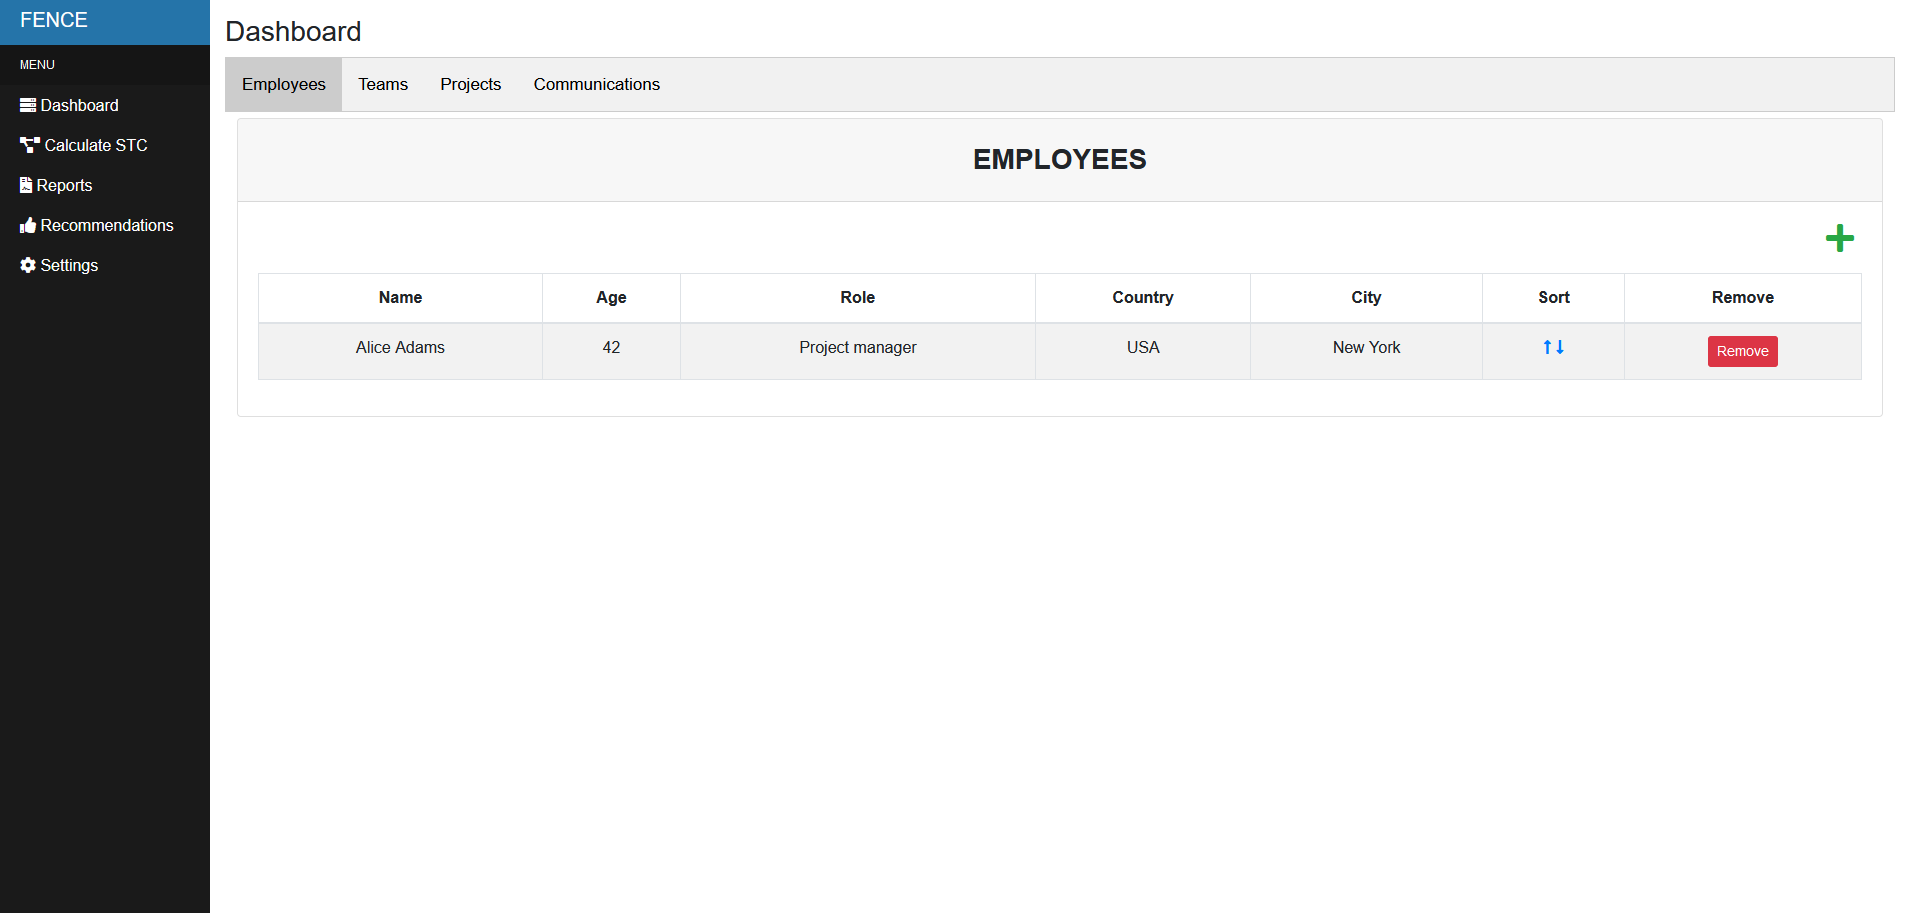
\includegraphics[width=0.95\linewidth]{4_first-dashboard}
	\caption[First dashboard version]{First dashboard version}
	\label{fig:first-dashboard}
\end{figure}

On the other hand, a home page was developed with information about the utility, version, and authorship of FENCE, whose final version is shown in Figure~\ref{fig:home-page}.

\begin{figure}
	\centering
	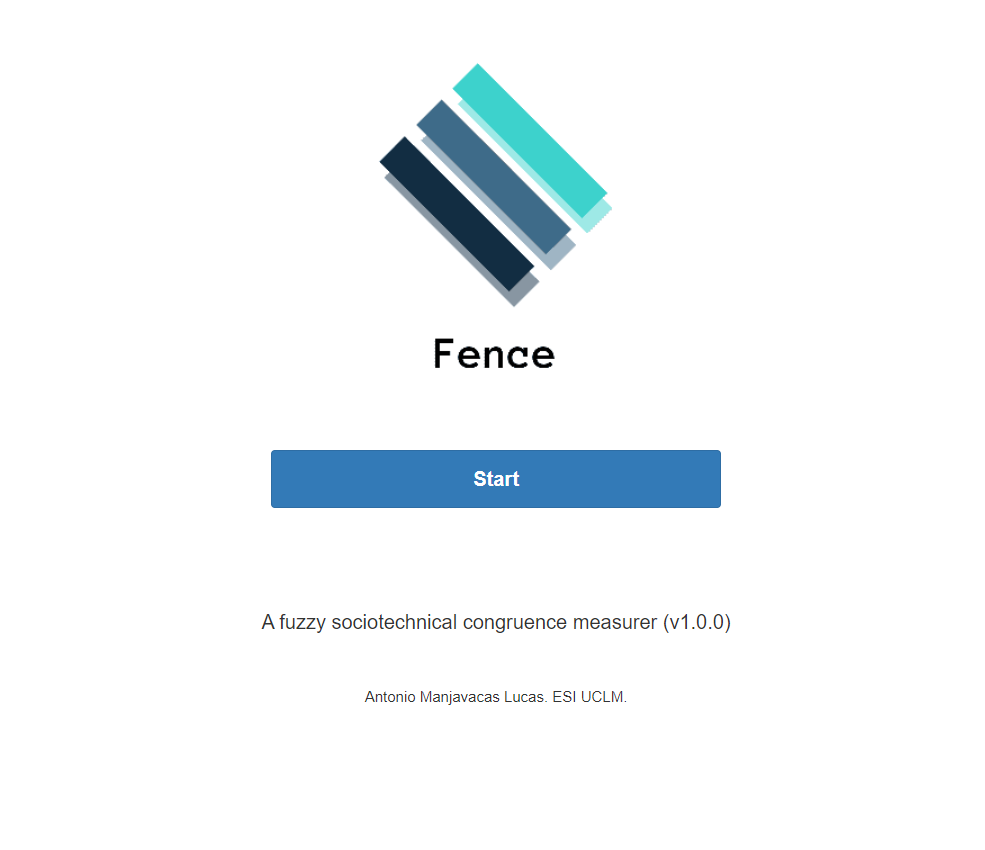
\includegraphics[width=0.8\linewidth]{4_home-page}
	\caption[FENCE home page]{FENCE home page}
	\label{fig:home-page}
\end{figure}

\subsection{Module 2. Main user interface}

In this second construction stage, efforts were focused on improving and completing the interface outlined in the previous module. This implied a greater deepening in HTML, CSS and JavaScript solutions, making use of Bootstrap and jQuery as nexus to implement the different functionalities of the interface. Initially, the use of these technologies never employed was an individual challenge, and therefore much of the effort invested at this stage was related with learning them.

An objective pursued in this stage was the elaboration of the different tabs and panels that compose the system's dashboard, as well as the communication between the interface and the application controllers via jQuery's Ajax requests. These requests were carried out according to the controllers' URIs defined in the previous construction stage, following the communication model expressed in Figure~\ref{fig:layer_int}.

\begin{figure}
	\centering
	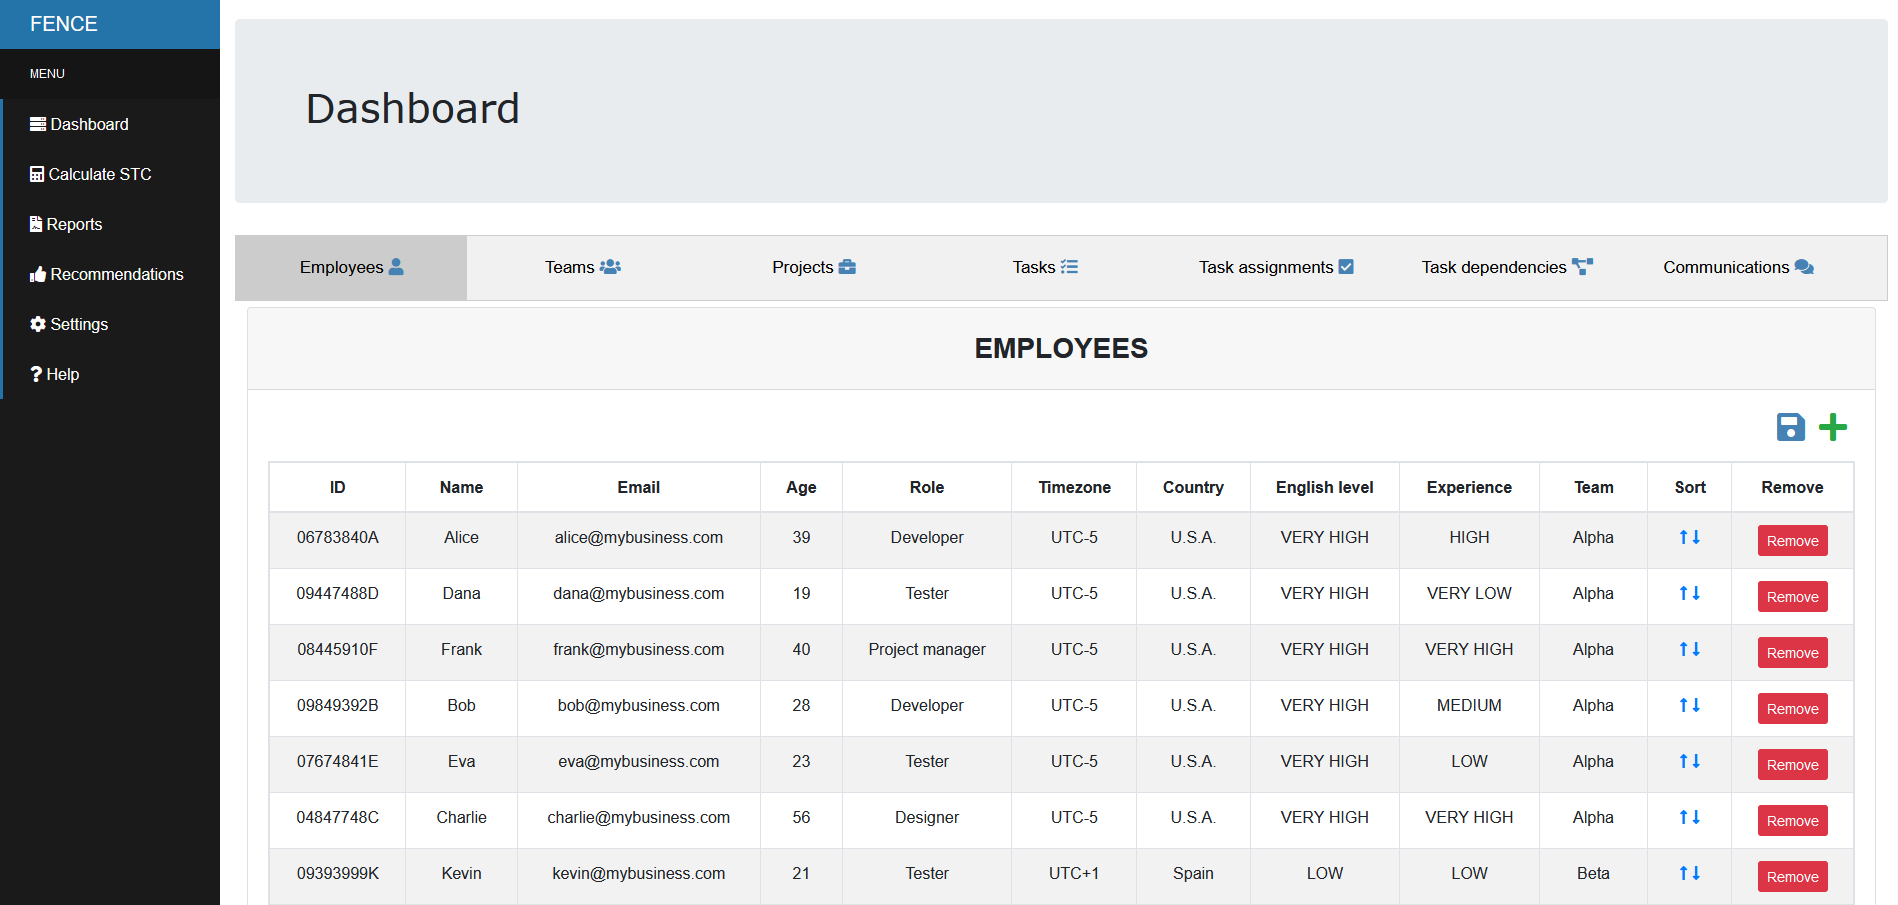
\includegraphics[width=0.95\linewidth]{4_fence-dashboard}
	\caption[FENCE dashboard]{FENCE dashboard}
	\label{fig:fence-dashboard}
\end{figure}

Furthermore, as can be seen in the Figure~\ref{fig:fence-dashboard}, these were the tabs contained the dashboard in its final version:

\begin{itemize}
	\item \textbf{Employees}: includes information on the users that are part of the organisation, used to measure individuals’ STC, such as age, experience, English level, country, etc.
	\item \textbf{Teams}: includes the name, location, and project membership of the different teams in the organization.
	\item \textbf{Projects}: active projects in the organization.
	\item \textbf{Tasks}: tasks to be carried out in each of the projects, together with their description, duration, priority, and completion.
	\item \textbf{Task assignments}: information about task assignment to users.
	\item \textbf{Task dependencies}: information on dependencies between tasks and their reliance weight.
	\item \textbf{Communications}: communications history between users. We will see in future sections their utility and how they are gathered.
\end{itemize}

Once the dashboard was implemented and the main application windows were set, some test data was loaded, while the proper performance of methods and queries were tested.

\subsection{Module 3. STC measurement}
\label{sec:stc}

Up to now, the creation of the main resources of the tool, their storage, and the CRUD interaction with them through the dashboard have been presented. In this stage, the objective pursued was to use these resources to carry out the measurement of the STC at the different levels of the organization under consideration: users, teams, and projects.

As previously explained in chapter \ref{cap:introduction}, the procedure taken as a reference to measure STC was the one exposed by Kwan et al. \cite{kwan_weighted_2009,kwan_does_2011}, given its facility to be adapted to the features and requirements of FENCE. Therefore, in the following subsection we will see gradually how the STC is calculated through the different algorithms implemented in this module:

\subsubsection{TASK ASSIGNMENT MATRIX ($T_A$)}

The first step in computing STC levels is to construct the task assignment matrix ($T_A$). This matrix matches tasks with users, representing the degree of user involvement in the tasks assigned to them (see Figure~\ref{fig:ta-matrix}).

\begin{figure}
	\centering
	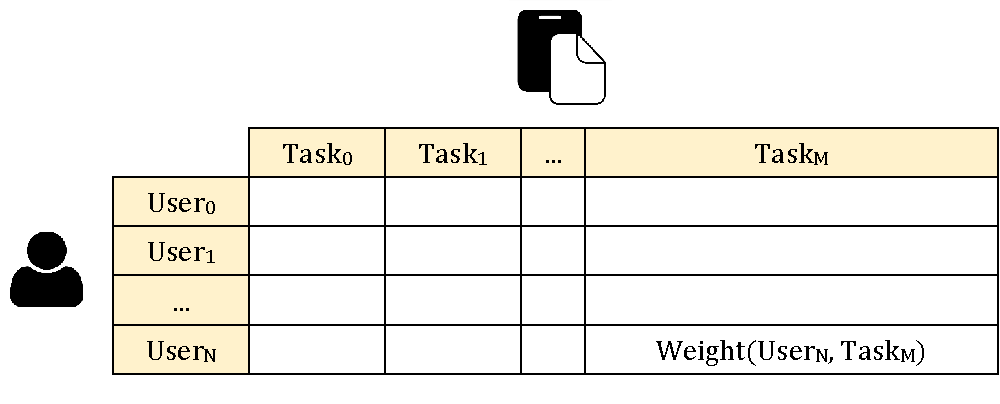
\includegraphics[width=0.95\linewidth]{4_ta-matrix}
	\caption[$T_A$ matrix]{$T_A$ matrix}
	\label{fig:ta-matrix}
\end{figure}

Both for this case and for the rest of the matrices detailed in the literature, in order to reduce the complexity and computational cost of the algorithms, these matrices were replaced by lists of objects stored in the database. In this case, the class $T_A$ represents a concrete cell in the $T_A$ matrix, as shown in Figure~\ref{fig:ta-class}. Moreover, the process carried out to fill in this matrix consists on the one shown in Algorithm~\ref{alg:ta}.

\begin{figure}
	\centering
	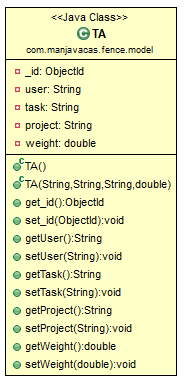
\includegraphics[width=0.32\linewidth]{4_ta-class}
	\caption[$T_A$ class]{$T_A$ class}
	\label{fig:ta-class}
\end{figure}

\begin{algorithm}
    
    \DontPrintSemicolon
    \SetKwInOut{Input}{input}
    \SetKwInOut{Output}{output}
    \Input{project}
    \Output{$T_A$ matrix}
    
    \caption{$T_A$ calculation}
    \label{alg:ta}
        
        $taMatrix \longleftarrow $\O$ $\;
        $tasks \longleftarrow getPendingTasks(project) $\;
        
        \ForEach{task $t$ in $tasks$}{
            $users \longleftarrow getUsersAssignedTo(task) $\;
            
            \If{users $\ne$ \O}{
                $sumExp \longleftarrow sumExperiences(users) $\;
                
                \ForEach{user $td$ in $users$}{
                    $weight \longleftarrow (user.experience / sumExp) * task.priority $\;
                    
                    \If{weight $>$ 1}{weight $\longleftarrow$ 1}
                    
                    $taMatrix \cup T_A(user, task, weight, project)$\;
                }
            }
        }
    
\end{algorithm}

Finally, the generated records are stored in the database replacing older ones, always keeping the most up-to-date $T_A$ matrix in the database.

\subsubsection{TASK DEPENDENCY MATRIX ($T_D$)}

The task dependency matrix ($T_D$) is very similar to the previous one, except that in this case the matrix does not relate users to tasks but tasks to each other. Specifically, what this matrix reflects is the degree of dependency between tasks in a project (see Figure~\ref{fig:td-matrix}). As this dependency level is flexible, it can be adapted to the user's understanding of "dependency". For example, the weight of the dependency between two tasks may reflect the number of functionalities of one task that must be previously implemented to perform the other.

\begin{figure}
	\centering
	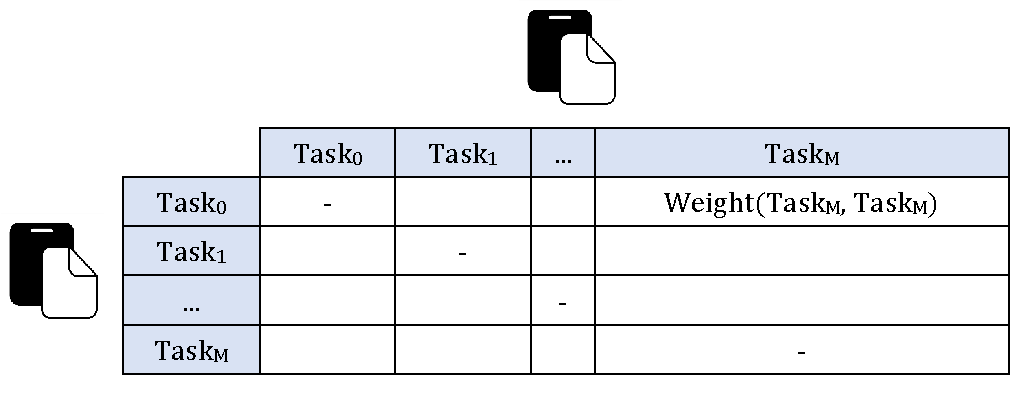
\includegraphics[width=0.95\linewidth]{4_td-matrix}
	\caption[$T_D$ matrix]{$T_D$ matrix}
	\label{fig:td-matrix}
\end{figure}

As in the previous case, the different cells of the $T_D$ matrix are stored as objects in the database (see Figure~\ref{fig:td-class}). The process of their creation is the one shown in Algorithm~\ref{alg:td}.

\begin{figure}
	\centering
	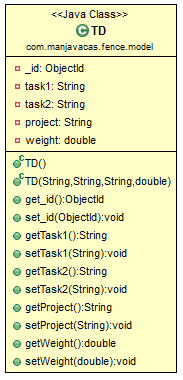
\includegraphics[width=0.32\linewidth]{4_td-class}
	\caption[$T_D$ class]{$T_D$ class}
	\label{fig:td-class}
\end{figure}

\begin{algorithm}
    
    \DontPrintSemicolon
    \SetKwInOut{Input}{input}
    \SetKwInOut{Output}{output}
    \Input{project}
    \Output{$T_D$ matrix}
    
    \caption{$T_D$ calculation}
    \label{alg:td}
        
        $tdMatrix \longleftarrow $\O$ $\;
        $tasks \longleftarrow getPendingTasksOf(project) $\;
        
        \ForEach{task $t$ in $tasks$}{
            $taskDependencies \longleftarrow getDependenciesOf(task) $\;
            
            \If{taskDependencies $\ne$ \O}{
                $sumValues \longleftarrow sumWeights(taskDependencies) $\;
                
                \ForEach{taskDependency $td$ in $taskDependencies$}{
                    $weight \longleftarrow td.weight / sumValues $\;
                    $tdMatrix \cup T_D(t, td, weight, project)$\;
                }
            }
        }
    
\end{algorithm}

Both the calculation of $T_D$ and $T_A$ is relatively quick, since the operations performed consist mainly on entering the information provided by the user in objects that are stored in the database. However, this is not the case of the $C_R$ and $C_A$ matrices, which will be presented in the following subsections.

\subsubsection{COMMUNICATION REQUIREMENTS MATRIX ($C_R$)}

Once the $T_A$ and $T_D$ matrices are obtained, we can compute the coordination requirements between users represented in the $C_R$ matrix (see Figure~\ref{fig:cr-matrix} and Figure~\ref{fig:cr-class}). This matrix represents the communication needs between user pairs based on the tasks assigned to them and their dependencies. In this case, the weights of the different matrix cells represent how much the users involved must coordinate.

\begin{figure}
	\centering
	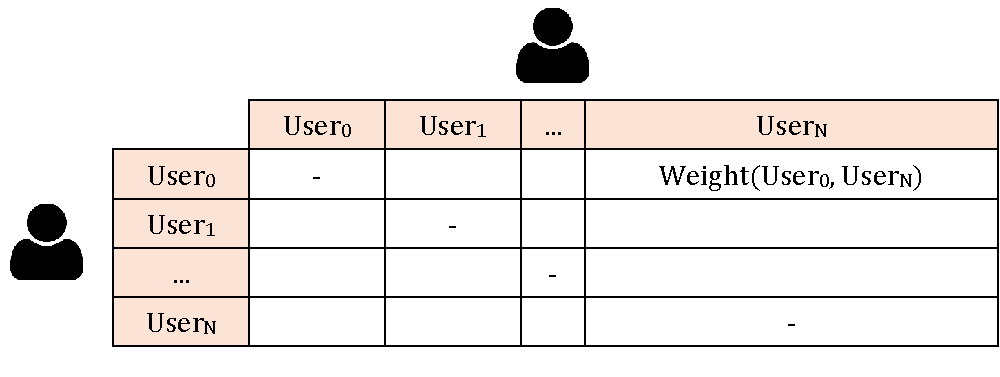
\includegraphics[width=0.95\linewidth]{4_cr-matrix}
	\caption[$C_R$ matrix]{$C_R$ matrix}
	\label{fig:cr-matrix}
\end{figure}

\begin{figure}
	\centering
	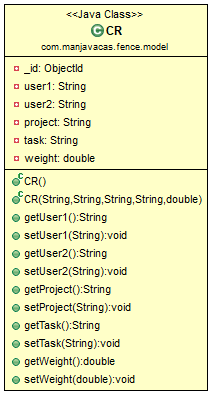
\includegraphics[width=0.32\linewidth]{4_cr-class}
	\caption[$C_R$ class]{$C_R$ class}
	\label{fig:cr-class}
\end{figure}

Initially calculated by means of the operations shown in Equation~\ref{eq:cr}, in this case we will follow an iterative procedure to calculate these coordination requirements, as no matrices are being used:

\begin{equation}
	\label{eq:cr}
	C_R = T_A * T_D * T_A^T
\end{equation}

As can be shown in Algorithm~\ref{alg:cr}, in the calculation of the weights for each coordination requirement, this weight is subsequently adjusted according to different distances present in Global Software Development projects. Thus, a fuzzy control system is used to carry out this adjustment, whose objective is none other than trying to reflect the difficulties or "penalties" to communication that may be caused by socio-cultural, geographical, or temporal distances among users.

\begin{algorithm}
    
    \DontPrintSemicolon
    \SetKwInOut{Input}{input}
    \SetKwInOut{Output}{output}
    \Input{project, $T_A$ matrix, $T_D$ matrix}
    \Output{$C_R$}
    
    \caption{$C_R$ calculation}
    \label{alg:cr}
        
        $crMatrix \longleftarrow $\O$ $\;
        
        \ForEach{ta $t$ in $taMatrix$}{
           
           $user_1 \longleftarrow ta.user $\;
           $dependencies \longleftarrow getDependenciesOf(ta.task) $\;
           
            \ForEach{taskDependency $td$ in dependencies}{
             
                $responsibles \longleftarrow getUsersAssignedTo(td.task_2)$\;
               
               \ForEach{user $user_2$ in responsibles} {
                    
                    \If{$user_2$ $\ne$ $user1$} {
                        $weight_{T_A}1 \longleftarrow ta.weight$ \;
                        $weight_{T_A}2 \longleftarrow T_A(td.task_2, user_2).weight$ \;
                        $weight_{T_D} \longleftarrow T_D(ta.task, td.task_2).weight$ \;
                        \;
                        $weight \longleftarrow weight_{T_A}1 * weight_{T_A}2 * weight_{T_D}$ \;
                        $weight \mathrel{{+}{=}} computeGlobalFactors(user_1, user_2)$ \;
                        \;
                        \If{weight $>$ 1}{weight $\longleftarrow$ 1}\;
                        $crMatrix \cup C_R(user_1, user_2, ta.task, weight, project)$\;
                    }
               }
               
            }
        }
    
\end{algorithm}

The entries taken by the fuzzy control system are the following:

\begin{itemize}
\item \textbf{Common English level}. Level of English shared by users, assuming that communication between them is always in this language despite their country provenance. It can be assumed that even if two users communicate in their native language, the level of English must be considered if the information disseminated by public chats (i.e. Jira, GitHub, Teams, Slack, etc.) should be interpretable by other users. Depending on the individual level of each user, the following weights are assessed:\newline

	\begin{itemize}
	\item If both users have a high level of English, the common level of English is 1.
	\item If one user has a high level and the other has a medium level, the weight is 0.7.
	\item If both have a medium level of English, the common level of English is 0.5.
	\item On the other hand, if one user has a medium level of English and the other has a low level, the resulting weight is 0.3.
	\item Finally, if both users have a low level of English the common weight is 0.\newline
	\end{itemize} 
	
	Moreover, the fuzzy sets associated with this variable are shown in the Figure~\ref{fig:fs-english}.\newline
	
	\begin{figure}
		\centering
		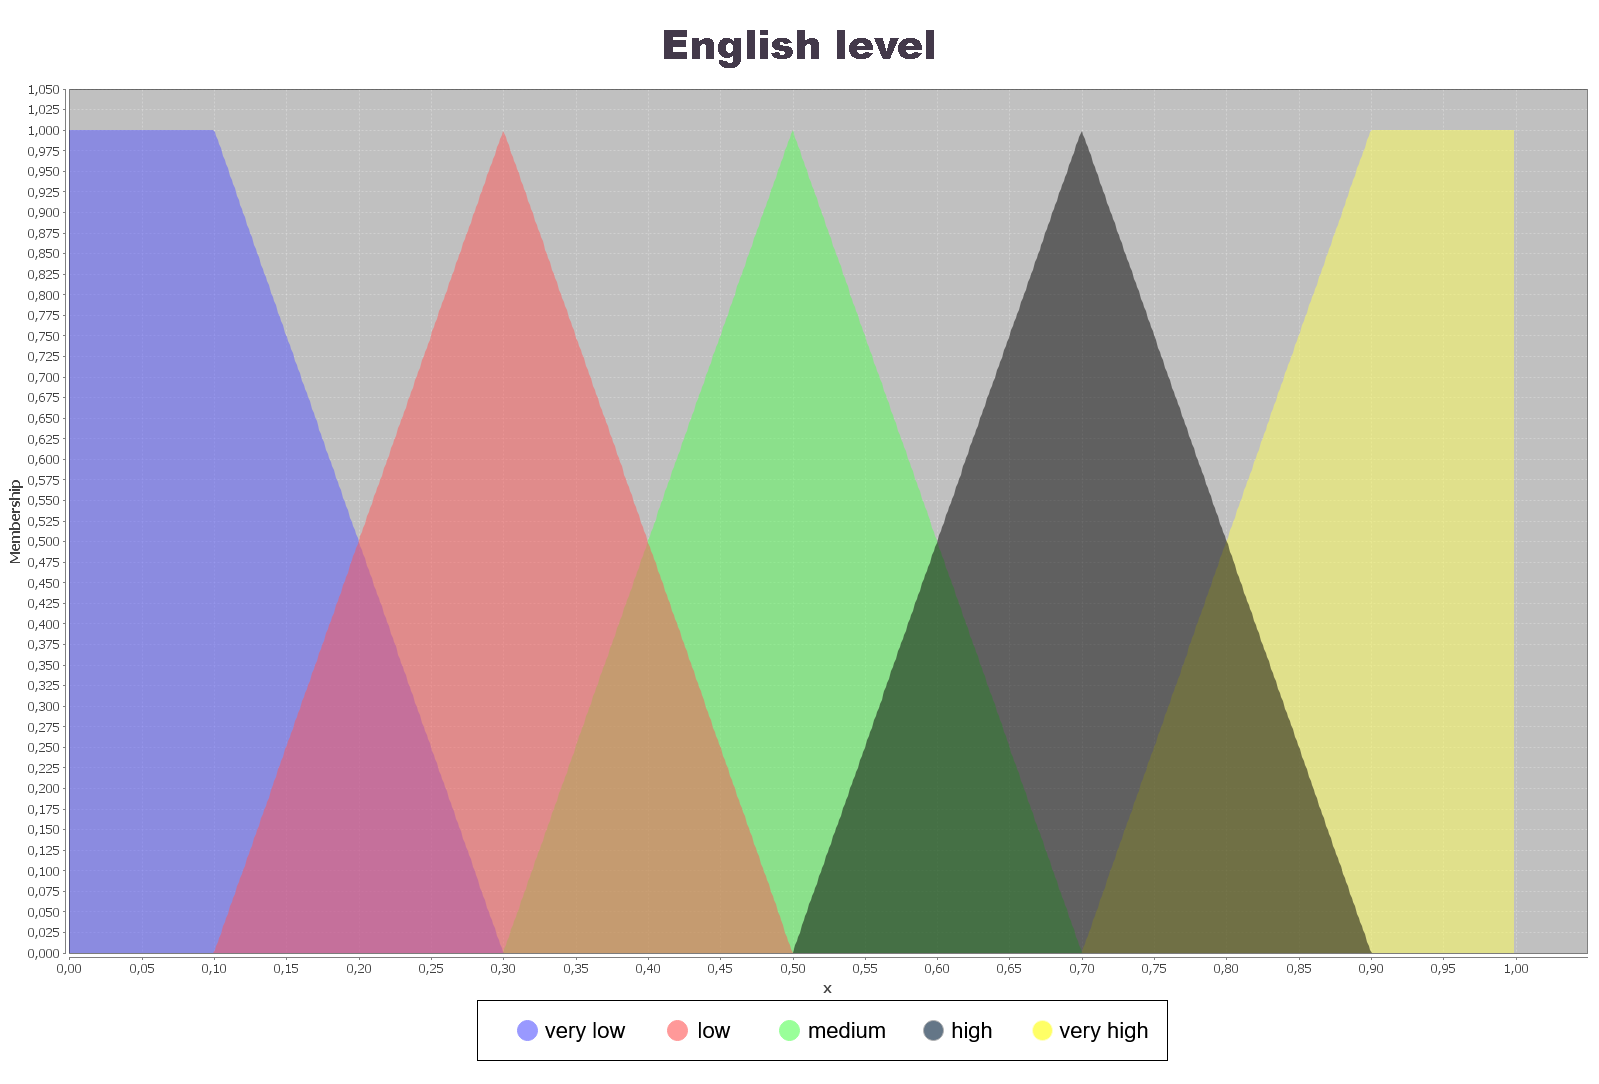
\includegraphics[width=0.9\linewidth]{4_fuzzy-sets-english}
		\caption[English level fuzzy sets]{English level fuzzy sets}
		\label{fig:fs-english}
	\end{figure}

\item \textbf{Cultural distance}. Average of the distances between socio-cultural factors identified by G. Hofstede \cite{hofstede_cultures_2004}, according to the employees’ nationality\footnote{These socio-cultural factors have been quantified by experts and are freely available for academic research purposes at \url{https://geerthofstede.com/research-and-vsm/dimension-data-matrix/}.}. These are the ones deeply explained in \cite{hofstede_dimensions}, \cite{hofstede_compare}:\newline

	\begin{itemize}
	\item \textbf{Power distance} (PDI): degree of acceptance of power differences or equality in society. In societies with higher PDI, higher social classes are more questioned, while in cultures with lower PDI, there is more equal power among people.
	\item \textbf{Individualism} (IDV): defines the level of integration of individuals into society and the development of a sense of group membership. Compared to more individualistic countries we find others with a collectivist orientation.
	\item \textbf{Masculinity} (MAS): defines a culture's tendency towards more masculine or feminine patterns of behaviour. According to Hofstede, male societies are more assertive, competitive and focused on outcomes than the generally more empathetic female societies.
	\item \textbf{Uncertainty avoidance} (UAI): acceptance of situations of uncertainty or where there is no absolute truth. It represents the degree of relativism of societies.
	\item \textbf{Long term orientation} (LTO): this cultural factor differentiates between more traditionalist societies, with long-term aspirations, and those with short-term orientations where social relations are seen as a means to gain some kind of benefit.
	\item \textbf{Indulgence} (IVR): explains the vision of life that every culture has. On the one hand, indulgent cultures tend to be more optimistic and positive than contained cultures. On the other hand, contained cultures consider a more reserved enjoyment.\newline
	\end{itemize}

	Thus, all these factors were inserted in a collection where each document represents a country with the cultural features differentiated in the mentioned study.\newline
	
	On this basis, the cultural distance (CD) is calculated by following the Equation~\ref{eq:cult-dist}.
	
	\begin{equation}
		\label{eq:cult-dist}
		CD = \frac{\left| pdi_1 - pdi_2 \right| + \left| idv_1 - idv_2 \right| + \left| mas_1 - mas_2 \right| + \left| uai_1 - uai_2 \right| + \left| lto_1 - lto_2 \right| + \left| ivr_1 - ivr_2 \right|}{6}
	\end{equation}
	
	Similarly, the fuzzy sets considered for this variable are shown in the Figure~\ref{fig:fs-cultural}.\newline

	\begin{figure}
		\centering
		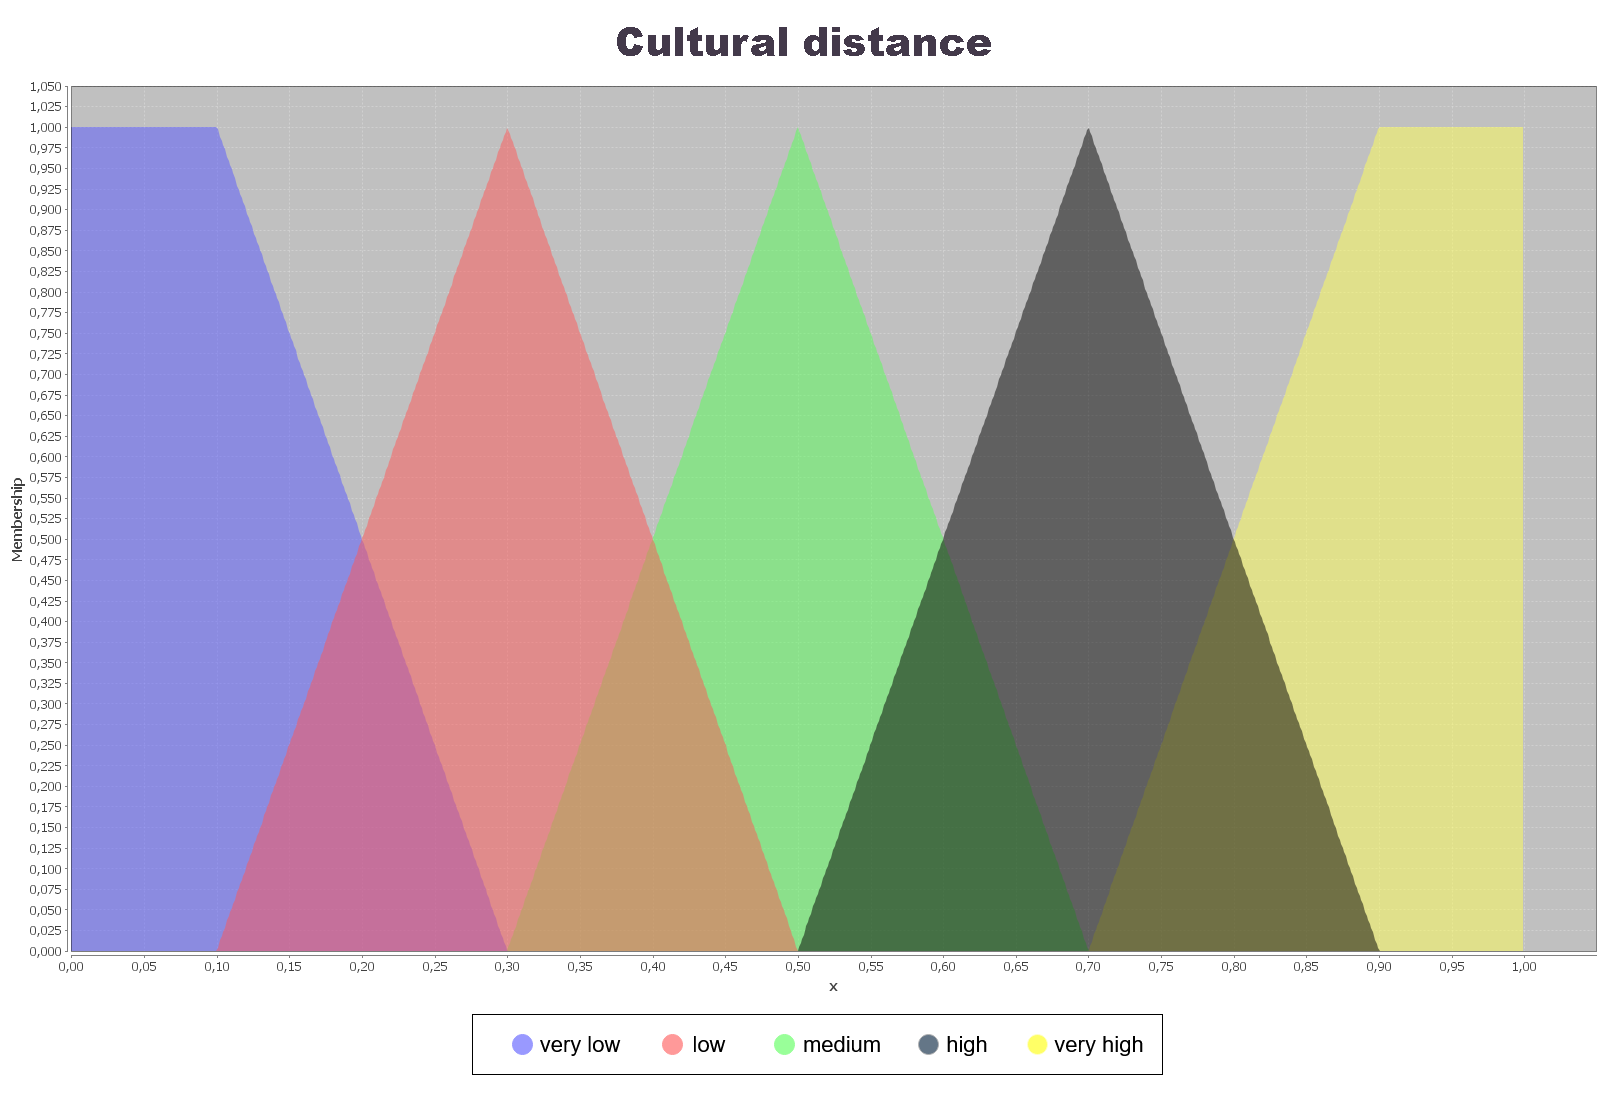
\includegraphics[width=0.9\linewidth]{4_fuzzy-sets-cultural}
		\caption[Cultural distance fuzzy sets]{Cultural distance fuzzy sets}
		\label{fig:fs-cultural}
	\end{figure}
	
\item \textbf{Time overlap}. Coincidence between employees’ time zones (UTC), calculated as the inverse of their time difference. A greater time overlap will facilitate the use of synchronous means of communication, while the impossibility of temporal coincidence in communication will result in greater use of asynchronous means. The computation of the time overlap is carried out following the Equation~\ref{eq:time-diff}, while the considered fuzzy sets for this input variable are shown in the Figure~\ref{fig:fs-time}.\newline

	\begin{equation}
		\label{eq:time-diff}
		TimeDiff = \left\{\begin{matrix}
		1 - \frac{UTC_1-UTC_2}{26}, UTC_1 \geq UTC_2
		\\
		\\
		1 - \frac{UTC_2-UTC_1}{26}, UTC_1 < UTC_2
		\end{matrix}\right.
	\end{equation}

	\begin{figure}
		\centering
		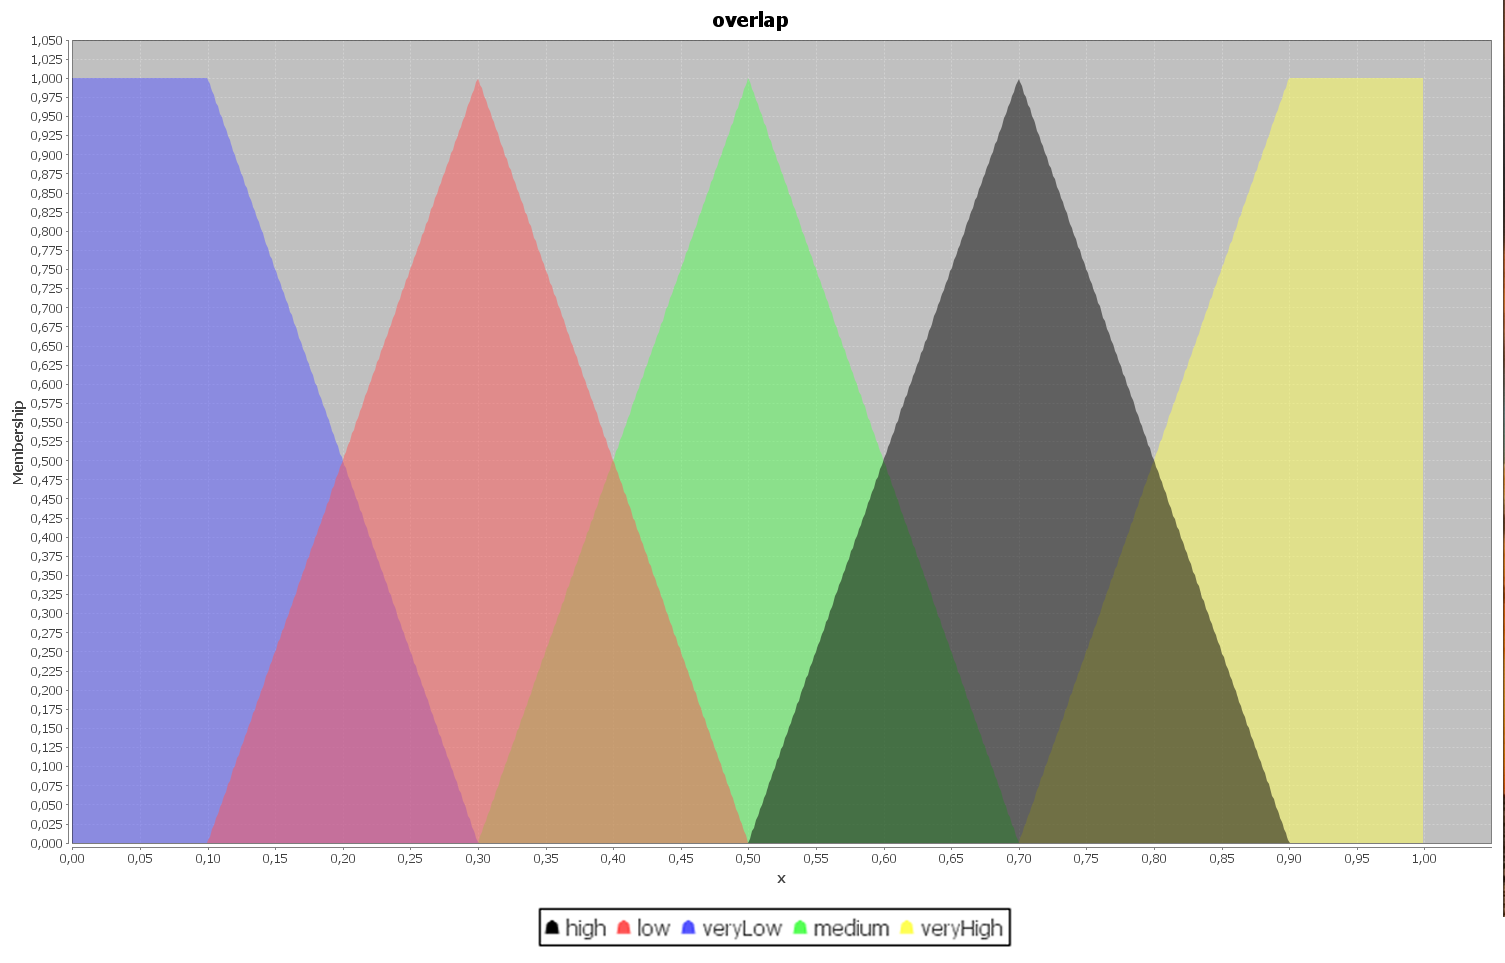
\includegraphics[width=0.9\linewidth]{4_fuzzy-sets-time}
		\caption[Time overlap fuzzy sets]{Time overlap fuzzy sets}
		\label{fig:fs-time}
	\end{figure}

	\vspace{16px}
	In turn, the set of rules defined using FCL and used by the system is displayed in Table~\ref{tb:cr-fuzzy-rules}.\newline
	
	\begin{table}
	\centering
	\caption{$C_R$ fuzzy control system rules}
	\label{tb:cr-fuzzy-rules}
	\resizebox{\textwidth}{!}{%
	\begin{tabular}{|c|l|}
	\hline
	\textbf{N} &
	  \multicolumn{1}{c|}{\textbf{FCL Rule}} \\ \hline\hline
	1 &
	  \begin{tabular}[c]{@{}l@{}}IF (culturalDist IS low OR culturalDist IS veryLow) AND (overlap IS low OR   overlap IS veryLow) \\ AND (englishLevel IS low OR englishLevel IS veryLow) THEN   modifier IS medium;\end{tabular} \\ \hline
	2 &
	  \begin{tabular}[c]{@{}l@{}}IF (culturalDist   IS low OR culturalDist IS veryLow) AND (overlap IS low OR overlap IS veryLow)   \\ AND (englishLevel IS medium OR englishLevel IS high OR englishLevel IS   veryHigh) THEN modifier IS medium;\end{tabular} \\ \hline
	3 &
	  \begin{tabular}[c]{@{}l@{}}IF   (culturalDist IS low OR culturalDist IS veryLow) AND (overlap IS medium) \\ AND (englishLevel IS low OR englishLevel IS veryLow) THEN modifier IS low;\end{tabular} \\ \hline
	4 &
	  \begin{tabular}[c]{@{}l@{}}IF (culturalDist IS low OR culturalDist IS veryLow) AND (overlap IS medium) AND  \\ (englishLevel IS medium OR englishLevel IS high OR englishLevel IS veryHigh) THEN   modifier IS medium;\end{tabular} \\ \hline
	5 &
	  \begin{tabular}[c]{@{}l@{}}IF   (culturalDist IS low OR culturalDist IS veryLow) AND (overlap IS high OR   overlap IS veryHigh) \\ AND (englishLevel IS low OR englishLevel IS veryLow)   THEN modifier IS veryLow;\end{tabular} \\ \hline
	6 &
	  \begin{tabular}[c]{@{}l@{}}IF   (culturalDist IS low OR culturalDist IS veryLow) AND (overlap IS high OR   overlap IS veryHigh) \\ AND (englishLevel IS medium OR englishLevel IS high OR   englishLevel IS veryHigh) THEN modifier IS veryLow;\end{tabular} \\ \hline
	7 &
	  \begin{tabular}[c]{@{}l@{}}IF   (culturalDist IS medium OR culturalDist IS high OR culturalDist IS veryHigh)   \\ AND (overlap IS low OR overlap IS veryLow) AND (englishLevel IS low OR   englishLevel is veryLow) THEN modifier IS veryHigh;\end{tabular} \\ \hline
	8 &
	  \begin{tabular}[c]{@{}l@{}}IF   (culturalDist IS medium OR culturalDist IS high OR culturalDist IS veryHigh)   AND (overlap IS low OR overlap IS veryLow) \\ AND (englishLevel IS medium OR   englishLevel IS high OR englishLevel IS veryHigh) THEN modifier IS high;\end{tabular} \\ \hline
	9 &
	  \begin{tabular}[c]{@{}l@{}}IF   (culturalDist IS medium OR    culturalDist IS high OR culturalDist IS veryHigh) AND (overlap IS   medium) \\ AND (englishLevel IS low OR englishLevel is veryLow) THEN modifier IS   veryHigh;\end{tabular} \\ \hline
	10 &
	  \begin{tabular}[c]{@{}l@{}}IF   (culturalDist IS medium OR culturalDist IS high OR culturalDist IS veryHigh)   AND (overlap IS medium)\\ AND (englishLevel IS medium OR englishLevel IS high   OR englishLevel IS veryHigh) THEN modifier IS medium;\end{tabular} \\ \hline
	11 &
	  \begin{tabular}[c]{@{}l@{}}IF (culturalDist   IS medium OR culturalDist IS high OR culturalDist IS veryHigh) AND (overlap   IS high OR overlap IS veryHigh) \\ AND (englishLevel IS low OR englishLevel is   veryLow) THEN modifier IS high;\end{tabular} \\ \hline
	12 &
	  \begin{tabular}[c]{@{}l@{}}IF   (culturalDist IS medium OR culturalDist IS high OR culturalDist IS veryHigh)   AND (overlap IS high OR overlap IS veryHigh) \\ AND (englishLevel IS medium OR   englishLevel IS high OR englishLevel IS veryHigh) THEN modifier IS medium;\end{tabular} \\ \hline
	\end{tabular}%
	}
	\end{table}
	
	After evaluating the rules, the output produced and conveniently defuzzified by the system will be the value to be added to the original $C_R$ weight. This penalty will attempt to represent the additional communication efforts that must be made between users due to the temporal, geographical and cultural distances between them.\newline
	
	Having studied how this fuzzy inference system works, it will be easily noted how the calculation of the $C_A$ matrix will make use of it in a very similar manner.

\end{itemize}

\subsubsection{ACTUAL COMMUNICATION MATRIX ($C_A$)}

When representing how users are trying to coordinate, it is necessary to take into account the communications between them. The actual coordination matrix ($C_A$) makes use of the communications within the organization to represent those pairs of users who have communicated, as shown in Figure~\ref{fig:ca-matrix}. Thus, the different cells of the $C_A$ matrix will represent with their weights how much communication has existed between each pair of users in a given project, being these communications related to concrete tasks (see Figure~\ref{fig:ca-class}.

\begin{figure}
	\centering
	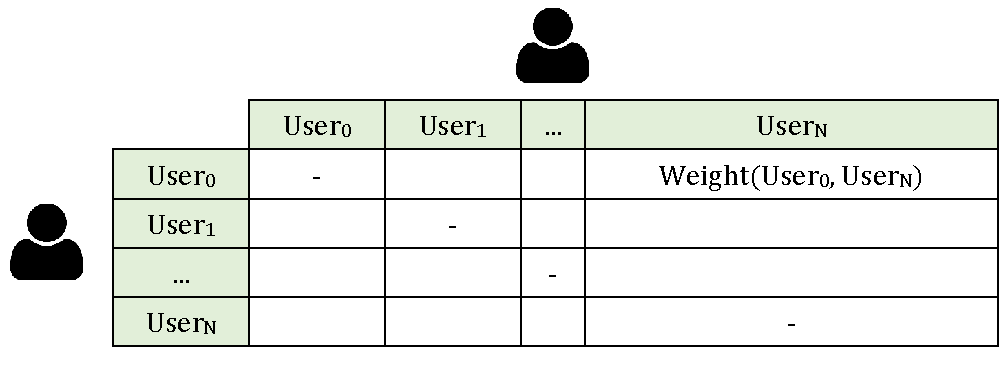
\includegraphics[width=0.95\linewidth]{4_ca-matrix}
	\caption[$C_A$ matrix]{$C_A$ matrix}
	\label{fig:ca-matrix}
\end{figure}

\begin{figure}
	\centering
	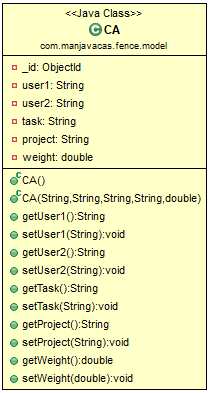
\includegraphics[width=0.32\linewidth]{4_ca-class}
	\caption[$C_A$ class]{$C_A$ class}
	\label{fig:ca-class}
\end{figure}

Before addressing the calculation of the $C_A$ objects stored in the database, it is necessary to clarify how the communications have been obtained to test the algorithm. In order to roughly simulate communications between users in the organization, a Python script was initially used to generate completely random conversations for a given project. However, after multiple iterations it was determined that the generated conversations hardly represented realistic communications, as the number of really useful communications to be generated was simply anecdotal. As a result, the script was consciously modified, giving rise to the one shown in Annex \ref{cap:annexA}, which in this case did provide more realistic and useful results when testing the tool. As can be seen, the script makes use of the existing coordination requirements in $C_R$ matrix and tries to fulfil them with a random amount of conversations between users. These communications would be stored in the database and used by the $C_A$ matrix algorithm detailed in Algorithm~\ref{alg:ca}.

\begin{algorithm}
    
    \DontPrintSemicolon
    \SetKwInOut{Input}{input}
    \SetKwInOut{Output}{output}
    \Input{project, $C_R$ matrix}
    \Output{$C_A$ matrix}
    
    \caption{$C_A$ calculation}
    \label{alg:ca}
        
        $caMatrix \longleftarrow $\O$ $\;
        $users \longleftarrow getUsers{C_R}()$\;
        
        \ForEach{user $user_1$ in $users$}{
        
            $weight_{C_A} \longleftarrow 0$\;
            $userTasks \longleftarrow getTasksAssignedTo(user_1)$\;
            $userCommunications \longleftarrow getCommunicationsOf(user_1)$\; 
            
            \ForEach{communication $com$ in $userCommunications$}{
            
                $user_2 \longleftarrow getUser_2(com)$\;
                $numDependencies \longleftarrow totalDependencies(user_1,user_2)$\;
                
                \If{numDependencies $>$ 0} {
                
                    $communications \longleftarrow getCommunicationsBetween(user_1,user_2)$\;
                    $totalCommunications \longleftarrow |communications|$\;
                    $taskCommunications \longleftarrow getTaskCommunications(com.task, communications)$\;
                    
                    \;
                    \If{taskCommunications $>$ 0}{
                        
                        \uIf{taskCommunications $\geq$ 5}{
                            $frequency \longleftarrow 1$\;
                        } \uElseIf{taskCommunications $\geq$ 3}{
                            $frequency \longleftarrow 0.6$\;
                        } \uElse{
                            $frequency \longleftarrow 0.3$\;
                        }
                    
                    }\;
                    
                    $weight_{C_A} \mathrel{{+}{=}} (frequency * totalCommunications / numDependencies)$\;
                    $weight_{C_A} \mathrel{{-}{=}} computeGlobalFactors(user_1,user_2)$\;
                    
                    \;
                    \If{$weight_{C_A}$ $>$ 1}{$weight_{C_A}$ $\longleftarrow$ 1}\;
                    
                    $caMatrix \cup C_A(user_1,user_2,com.task,weight_{C_A},project)$\;
                
                }
            
            }
        
        }
    
\end{algorithm}

In this case, the fuzzy inference system is used to adjust the weight obtained. As can be noted, the penalty for temporal, geographical and cultural distances will result in the decrease of the weight, subtracting part of the value of the established communications.

It can also be observed that the calculation of this matrix is the most time-consuming comparing to the other matrices, and that is because the execution of the algorithm depends on relatively large input data, such as users in $C_R$, communications and tasks. However, by following this process, we will have calculated the $C_A$ matrix and will be ready to compare the current communication with the existing coordination requirements.

\subsubsection{COORDINATION GAPS MATRIX ($C_G$)}

The last matrix to be calculated, which will lead us to compute STC, is the coordination gaps matrix ($C_G$). This matrix represents in its cells the difference between the communication that each pair of users must achieve and the communication that is actually taking place (see Figure~\ref{fig:ca-matrix} and Figure~\ref{fig:ca-class}). In other words, each cell of the $C_G$ array for users $user_i$ and $user_j$ represents the difference in weight between $C_R$($user_i$, $user_j$) and $C_A$($user_i$, $user_j$). As can be observed, the weights of the $C_G$ matrix clearly represent the coordination requirements that are being covered as well as those communication gaps that are still present between users.

\begin{figure}
	\centering
	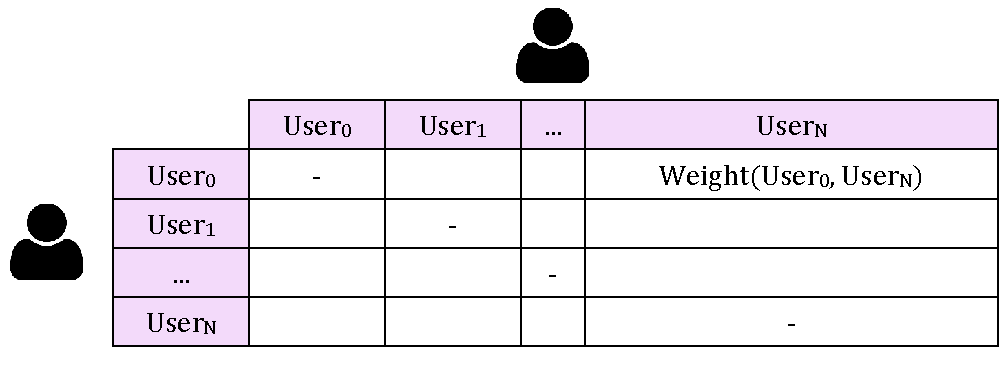
\includegraphics[width=0.95\linewidth]{4_cg-matrix}
	\caption[$C_G$ matrix]{$C_G$ matrix}
	\label{fig:cg-matrix}
\end{figure}

\begin{figure}
	\centering
	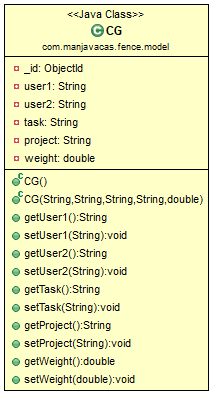
\includegraphics[width=0.32\linewidth]{4_cg-class}
	\caption[$C_G$ class]{$C_G$ class}
	\label{fig:cg-class}
\end{figure}

The procedure followed to fill in this matrix is relatively simple compared to the previous ones, as can be observed in Algorithm~\ref{alg:cg}.

\begin{algorithm}
    
    \DontPrintSemicolon
    \SetKwInOut{Input}{input}
    \SetKwInOut{Output}{output}
    \Input{$C_A$ matrix, $C_R$ matrix}
    \Output{$C_G$ matrix}
    
    \caption{$C_G$ calculation}
    \label{alg:cg}
        
        $cgMatrix \longleftarrow $\O$ $\;
       
        \ForEach{$cr$ in $crMatrix$}{
            $caList \longleftarrow getCA(cr.user_1,cr.user_2,cr.project,cr.task)$\;
            
            \uIf{caList $\ne$ \O}{
               $weight_{C_A} \longleftarrow sumWeights(caList)$\;
               $weight_{C_R} \longleftarrow cr.weight$\;
               $weight_{C_G} \longleftarrow weight_{C_R} - weight_{C_A}$\;
               
               \If{$weight_{C_G}$ $>$ 0} {
                    $cgMatrix \cup C_G(cr.user_1, cr.user_2, cr.task, weight_{C_G}, cr.project)$\;
               }
            }\Else{
                $cgMatrix \cup CG(cr.user_1, cr.user_2, cr.task, cr.weight, cr.project)$\;
            }
        }
    
\end{algorithm}

With the $C_G$ matrix representing the lack of coordination between users in a given project, the calculation of the organisation's STC levels will then be undertaken.

\subsubsection{SOCIOTECHNICAL CONGRUENCE MEASUREMENT}

As we have already indicated, the requirements to be met by FENCE involve the calculation of STC levels from three different points of view: employees, teams, and projects. As we shall see below, knowing the STC level of the organisation's teams and projects is relatively simple, being the obtainment of the employees' STC levels the basis of this calculations.

\begin{itemize}
\item \textbf{Employees' STC}
\end{itemize}

To calculate the individual STC of each user we will follow the process detailed in Algorithm~\ref{alg:stc-user}, where Equation~\ref{eq:stc-user} will be used to calculate the individual level of STC for each employee.

\begin{algorithm}
    
    \DontPrintSemicolon
    \SetKwInOut{Input}{input}
    \SetKwInOut{Output}{output}
    \Input{project, $C_R$ Matrix, $C_G$ matrix}
    \Output{users STC}
    
    \caption{User STC calculation}
    \label{alg:stc-user}
        
        $stcUsers \longleftarrow $\O$ $\;
        $users \longleftarrow getProjectUsers(project)$\;
        
        \ForEach{$user$ in $users$}{
            $userCRs \longleftarrow getUserCRs(user)$\;
            $userCGs \longleftarrow getUserCGs(user)$\;
            
            $userCRsum \longleftarrow sumWeights(userCRs)$\;
            $userCGsum \longleftarrow sumWeights(userCGs)$\;
            
            \uIf{userCGsum $\leq$ 0} {
                $stcUsers \cup UserSTC(user, 100.0, getCurrentDate())$\;
            }\Else{
                $stcUser \longleftarrow 1 - (userCGsum / userCRsum)$\;
                $stcUsers \cup UserSTC(user, stcUser * 100, getCurrentDate())$\;
            }
        }
        
\end{algorithm}


\begin{equation}
\label{eq:stc-user}
STC = 1 - \frac{\sum_{i=0}^{n}\sum_{j=0}^{n}C_{Gij}}{\sum_{i=0}^{n}\sum_{j=0}^{n}C_{Rij}}
\end{equation}

At the same time, note how each measurement will be dated. This will allow us to have a history of the STC levels for each user, team, and project, whose usefulness will be seen in the next module.

\begin{itemize}
\item \textbf{Teams' STC}
\end{itemize}

In this case, as shown in Algorithm~\ref{alg:stc-team}, the calculation of the STC at team level is very similar to the previous one, except that the users considered are those belonging to the chosen team.

\begin{algorithm}
    
    \DontPrintSemicolon
    \SetKwInOut{Input}{input}
    \SetKwInOut{Output}{output}
    \Input{project, $C_R$ Matrix, $C_G$ matrix}
    \Output{teams STC}
    
    \caption{Teams STC calculation}
    \label{alg:stc-team}
        
        $stcTeams \longleftarrow $\O$ $\;
        $teams \longleftarrow getProjectTeams(project)$\;
        
        \ForEach{$team$ in $teams$}{
            $teamCRsum \longleftarrow 0 $\;
            $teamCGsum \longleftarrow 0 $\;
            $teamUsers \longleftarrow team.users$\;
            
            \ForEach{$user$ in $teamUsers$}{
            
                $userCRs \longleftarrow getUserCRs(user)$\;
                $userCGs \longleftarrow getUserCGs(user)$\;
                
                $teamCRsum \mathrel{{+}{=}} sumWeights(userCRs)$\;
                $teamCGsum \mathrel{{+}{=}} sumWeights(userCGs)$\;
                
            }  
            
            \uIf{teamCGsum $\leq$ 0} {
                $stcTeams \cup TeamSTC(team, 100.0, getCurrentDate())$\;
            }\Else{
                $stcTeam \longleftarrow 1 - (teamCGsum / teamCRsum)$\;
                $stcTeams \cup TeamSTC(team, stcTeam * 100, getCurrentDate())$\;
            }
        }  
    
    \end{algorithm}

As in the previous case, we will keep a history of the STC measurements for teams.

\begin{itemize}
\item \textbf{Project STC}
\end{itemize}

Having calculated the STC at user and team level, it only remains to measure it at project level by following the process detailed in Algorithm~\ref{alg:stc-project}.

\begin{algorithm}
    
    \DontPrintSemicolon
    \SetKwInOut{Input}{input}
    \SetKwInOut{Output}{output}
    \Input{project, $C_R$ Matrix, $C_G$ matrix}
    \Output{project STC}
    
    \caption{Project STC calculation}
    \label{alg:stc-project}
        
        $projectCRsum \longleftarrow sumWeights(C_R)$\;
        $projectCGsum \longleftarrow sumWeights(C_G)$\;
        
        \uIf{projectCGsumt $\leq$ 0} {
            $stcProject \cup ProjectsSTC(team, 100.0, getCurrentDate())$\;
        }\Else{
            $stcProject \longleftarrow 1 - (projectCGsum / projectCRsum)$\;
            $stcProject \cup ProjectSTC(project, stcProject * 100, getCurrentDate())$\;
        }
        
    \end{algorithm}

Once seen in detail the implementation of the algorithms and their adaptation to the information handled by FENCE, it only remains to illustrate how the information is requested by the user and displayed in the interface (see Figure~\ref{fig:stc-measurer}.

\begin{figure}
	\centering
	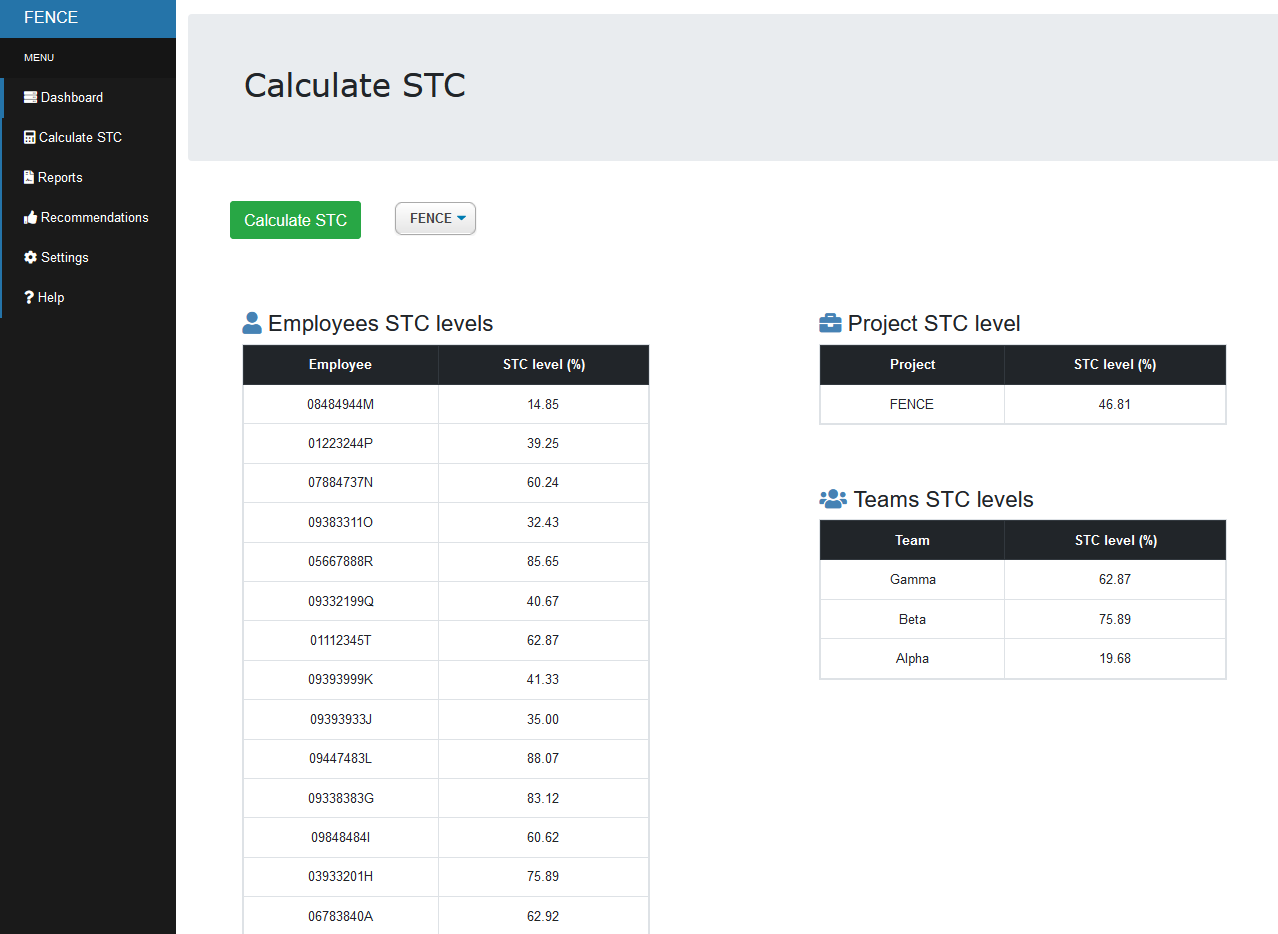
\includegraphics[width=0.95\linewidth]{4_stc-measurer}
	\caption[STC measurer interface]{STC measurer interface}
	\label{fig:stc-measurer}
\end{figure}

\begin{itemize}
\item Initially, when the user accesses the STC tab, the last measurements made by the tool will be loaded into the different tables: users, teams, and project tables. 
\item If the user wants to recalculate the STC levels for a given project, he or she must select it and directly click on the "Calculate STC" button. 
\item This will cause the STC levels to be recalculated, along with the values from the different matrices, being also updated in the database. 
\item Finally, once this process is completed, the tables will be filled with the most updated version of the STC levels.
\end{itemize}

As can be noted, new resources such as classes to model STC measurements and matrices were included and implemented in this phase, while others previously defined were expanded or adjusted to the needs of the STC meter.

It also should be considered that the entire execution of the STC calculation algorithm is quite computational costly. Although this complexity was iteratively reduced, resulting in significantly better performance, the amount of time required for execution remained considerable given the complexity of the calculations to be made and the number of inputs (users, tasks, assignments, dependencies, communications) to be handled.

Nevertheless, the results provided by the system developed in this module would serve as a basis for the development and use of the following modules, focused on visualizing and improving the organization's STC levels.

\subsection{Module 4. Data visualization}

The objective of the work carried out in this module was to allow the visualization of time series with information on STC measurements in employees, teams, and projects. Based on this, the implementation of the graphics was carried out using the JavaScript library \emph{Chart.js}.

This library offers a flexible and simple way to generate many types of charts. In this case, the input data would be displayed in a timeline, corresponding to the latest STC measurements for each employee, team, and project.

Looking at the FENCE interface, as can be seen in Figure~\ref{fig:reports}, the user will find three canvas with which he or she can interact by selecting at convenience the specific employee, team or project from which it is desired to know its STC history levels.

\begin{figure}
	\centering
	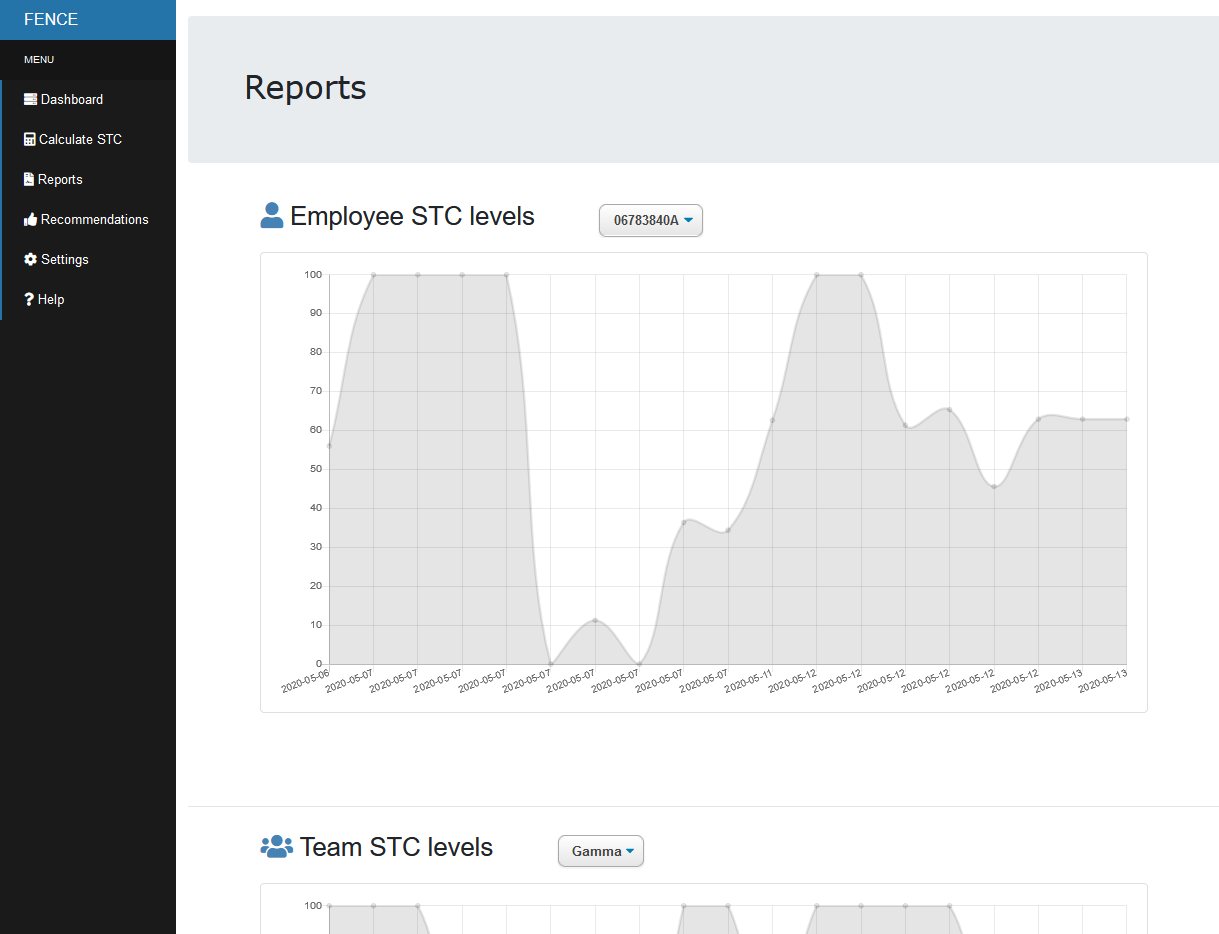
\includegraphics[width=0.95\linewidth]{4_reports}
	\caption[Reports interface]{Reports interface}
	\label{fig:reports}
\end{figure}

If we go deeper into the construction and operation of the charts beyond the interface, initially the application makes GET-type Ajax requests to the corresponding controllers. Each controller shown in Figure~\ref{fig:measurements-controllers} receives the request and invokes the corresponding method in the associated service object (see Figure~\ref{fig:measurements-services}), which retrieves and returns all the measurements stored in the database. When each AJAX request receives the result of the query, the last 20 measurements performed are extracted and entered as input data to be represented by the \emph{Chart.js} plot.

\begin{figure}
	\centering
	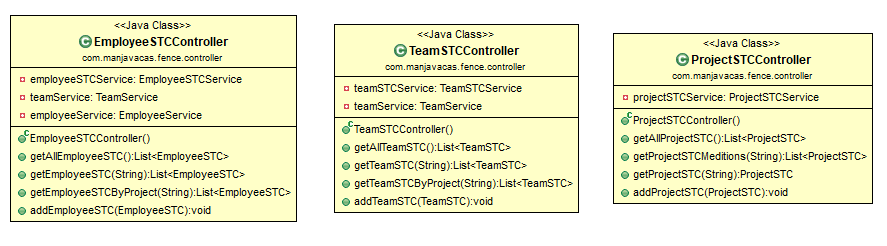
\includegraphics[width=0.95\linewidth]{4_controllers-measurement}
	\caption[STC measurements controllers]{STC measurements controllers}
	\label{fig:measurements-controllers}
\end{figure}

\begin{figure}
	\centering
	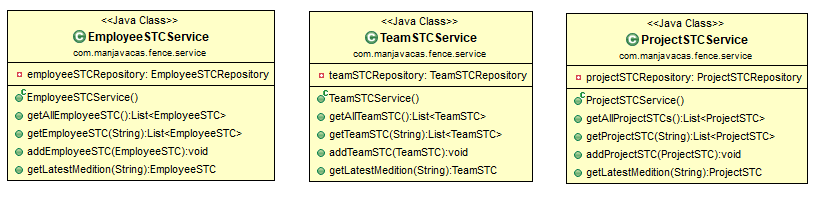
\includegraphics[width=0.95\linewidth]{4_services-measurement}
	\caption[STC measurements services]{STC measurements services}
	\label{fig:measurements-services}
\end{figure}

This is a fast and simple process, which provides FENCE with more analytical capabilities for the analysis of STC levels evolution. Visualising this progression can help project managers, or even strategic leaders, to consider what issues are affecting the performance of the global projects. 

Once this phase based on data visualisation has been overcome, the next module would allow to undertake concrete actions to improve the STC levels within the organisation.

\subsection{Module 5. Recommendation system}

This module addressed the development of one of the main and most distinctive functionalities of FENCE: the development of a recommendation system focused on providing information to the user about how to improve the STC levels of the organization.

Before starting the development of this system, meetings were held with the different stakeholders:

\subsubsection{TECHNICAL PLANNING}
Initially, it was discussed through different meetings with José Ángel Olivas how to approach the development of the recommendation system by using the information provided by FENCE. It was agreed that the coordination gap matrix (CG) was ideal for finding out which users were those on whom recommendations should be made. Moreover, the variables and rules to be used by the fuzzy inference system were also studied and initially outlined.

After these sessions, multiple alternatives were considered when working with fuzzy logic in Java, being finally jFuzzyLogic \cite{cingolani_jfuzzylogic_2012, cingolani_jfuzzylogic_2013} the library chosen for this task. This library is based on the definition of fuzzy inference systems by means of the standard FCL \cite{FCL}, so it was necessary to learn its syntax in the handling of variables, functions, fuzzy sets, and rules.

The main features of this library that led to its use were: its flexibility and ease of integration with the system developed so far; the use of FCL (a relatively simple fuzzy definition language) as well as being quite updated in relation to other fuzzy logic libraries found.

With this technical base and once familiar with jFuzzyLogic after multiple tests, the knowledge engineering work was carried out together with the Aurora Vizcaíno, who played the role of expert.

\subsubsection{KNOWLEDGE ENGINEERING}

Knowledge engineering involves the extraction of expert knowledge and its translation into a formalized language in a precise, unambiguous, and exploitable way. On this basis, the knowledge engineering tasks performed would allow us to define the features that should be covered by the recommending system. 

If we consider its scope and limitations, the following ones were considered:

\begin{itemize}
	\item \textbf{Scope}: given the characteristics of the users that integrate the multiple teams on a given project, as well as the organization's STC levels, the system will offer as output recommendations to improve those STC levels in a clear and traceable way.
	\item \textbf{Limitations}: the number of features covered will be strictly limited to the knowledge of the expert. The system shall also not contemplate specific features of the project, teams and users going beyond the information provided as input.
\end{itemize}

Subsequently, once the domain of the system had been established, the choice of the expert willing to transmit her knowledge was made. In this case, as previously stated, it was Aurora Vizcaíno, university professor and researcher in the Computer Science School of Ciudad Real. It was considered that her contributions would be an important source of knowledge given her experience in the field of GSD, as well as her work in multiple research projects related to communication and knowledge management in this domain.

On the other hand, one of the main tasks of the knowledge engineer is the study of the viability of the project to be undertaken. One of the most recognised ways of studying this viability is the Slagel Test \cite{mate_1998}. This test is focused on the study of the plausibility, justification, success, adequacy, and success of expert systems, allowing to determine if the project is viable based on the reasoning over its characteristics:

\begin{itemize}
\item \textbf{Plausibility}: determines whether the necessary means to address the problem from the perspective of Knowledge Engineering are available. From this point of view, the characteristics of the expert and the task to be undertaken are analysed.
\item \textbf{Justification}: analysis of the need for experience and the investment to be made (type of environment, need due to volatile experience, return of investment, alternative solutions, etc.).
\item \textbf{Adequacy}: it is studied if the problem is adequate to be solved with Knowledge Engineering techniques, analysing its nature, complexity, and type.
\item \textbf{Success}: the probabilities of the system's success are determined in advance. It involves studying non-technical but important issues in order to decide to apply Knowledge Engineering to the resolution of the problem, such as the involvement and responsibility of the people implicated, as well as the acceptance of the system in its environment.
\end{itemize}

In this way, the process conducted in order to justify the viability of the recommending system to be developed is shown below:

\begin{itemize}
\item First, for each of the dimensions mentioned, three different categories are established:

	\begin{itemize}
	\item Managers and/or users (MU).
	\item Experts (EX).
	\item Tasks (TA).
	\end{itemize}
	
	For each category, the most important features that define that dimension are specified. These features may be essential (E) or desirable (D), considering that essential features must not have a value below a threshold (7 in this case).
	
	On this basis, each feature is assigned a weight between 0 and 10, depending on its relative importance. This entire process is summarized in tables Table \ref{tb:plau}, Table \ref{tb:just}, Table \ref{tb:adeq}, and Table \ref{tb:suc}.

\begin{table}[]
	\centering
	\caption[Plausability study]{Plausability study}
	\label{tb:plau}
	\resizebox{\textwidth}{!}{%
	\begin{tabular}{|c|c|c|c|l|c|}
	\hline
	\multicolumn{6}{|c|}{\textbf{Plausibility}} \\ \hline\hline
	\textbf{Category} &
	  \textbf{Identifier} &
	  \textbf{Weight} &
	  \textbf{Value} &
	  \multicolumn{1}{c|}{\textbf{Feature definition}} &
	  \textbf{Type} \\ \hline\hline
	EX &
	  P1 &
	  10 &
	  8 &
	  Experts    exist &
	  E \\ \hline
	EX &
	  P2 &
	  10 &
	  9 &
	  The    assigned expert is genuine &
	  E \\ \hline
	EX &
	  P3 &
	  8 &
	  10 &
	  The    expert is cooperative &
	  D \\ \hline
	EX &
	  P4 &
	  7 &
	  9 &
	  \begin{tabular}[c]{@{}l@{}}The expert    is able to articulate his/her methods, \\ but does not categorize\end{tabular} &
	  D \\ \hline
	TA &
	  P5 &
	  10 &
	  8 &
	  There    are enough test cases &
	  E \\ \hline
	TA &
	  P6 &
	  10 &
	  9 &
	  The    task is well structured and understood &
	  D \\ \hline
	TA &
	  P7 &
	  10 &
	  8 &
	  It    only requires cognitive ability &
	  D \\ \hline
	TA & P8 & 9 & 8 & \begin{tabular}[c]{@{}l@{}}No    optimal results are required but only satisfactory ones, \\ without    compromising the project\end{tabular} & D \\ \hline
	TA &
	  P9 &
	  9 &
	  7 &
	  The    task does not require common sense &
	  D \\ \hline
	DU &
	  P10 &
	  7 &
	  10 &
	  The    managers are truly committed to the project &
	  D \\ \hline
	\end{tabular}%
	}
\end{table}

\begin{table}[]
	\centering
	\caption[Justification study]{Justification study}
	\label{tb:just}
	\resizebox{\textwidth}{!}{%
	\begin{tabular}{|c|c|c|c|l|c|}
	\hline
	\multicolumn{6}{|c|}{\textbf{Justification}}                                        \\ \hline\hline
	\textbf{Category} &
	  \textbf{Identifier} &
	  \textbf{Weight} &
	  \textbf{Value} &
	  \multicolumn{1}{c|}{\textbf{Feature definition}} &
	  \textbf{Type} \\ \hline\hline
	EX & J1 & 10 & 9 & The expert is   not available                                & E \\ \hline
	EX & J2 & 10 & 9 & There's a   shortage of human experience                     & D \\ \hline
	TA & J3 & 8  & 9 & There is a   need for simultaneous experience in many places & D \\ \hline
	TA &
	  J4 &
	  10 &
	  8 &
	  \begin{tabular}[c]{@{}l@{}}Need for   experience in hostile, distressing and/or \\ unrewarding environments\end{tabular} &
	  E \\ \hline
	TA & J5 & 8  & 9 & There are no   admissible alternative solutions              & E \\ \hline
	MU & J6 & 7  & 9 & A high rate of   return on investment is expected            & D \\ \hline
	MU & J7 & 8  & 9 & Solves a   useful and necessary task                         & E \\ \hline
	\end{tabular}%
	}
\end{table}

\begin{table}[]
	\centering
	\caption[Adequacy study]{Adequacy study}
	\label{tb:adeq}
	\resizebox{\textwidth}{!}{%
	\begin{tabular}{|c|c|c|c|l|c|}
	\hline
	\multicolumn{6}{|c|}{\textbf{Adequacy}}                                          \\ \hline\hline
	\textbf{Category} &
	  \textbf{Identifier} &
	  \textbf{Weight} &
	  \textbf{Value} &
	  \multicolumn{1}{c|}{\textbf{Feature definition}} &
	  \textbf{Type} \\ \hline\hline
	EX & A1  & 5 & 7  & The expert's   experience is poorly organized            & D \\ \hline
	TA & A2  & 6 & 7  & It has little   practical value                          & D \\ \hline
	TA & A3  & 7 & 7  & It is a more   tactical than strategic task              & D \\ \hline
	TA & A4  & 7 & 9  & The task   provides solutions that serve long-term needs & E \\ \hline
	TA &
	  A5 &
	  5 &
	  9 &
	  \begin{tabular}[c]{@{}l@{}}The task is   not too easy, but it is knowledge-intensive, \\ both in the domain and in the   manipulation of information\end{tabular} &
	  D \\ \hline
	TA &
	  A6 &
	  6 &
	  9 &
	  \begin{tabular}[c]{@{}l@{}}It is   manageable in size, and/or a gradual approach is possible and/or, \\ a breakdown   into independent sub-tasks\end{tabular} &
	  D \\ \hline
	EX & A7  & 7 & 10 & The transfer   of experience between humans is feasible  & E \\ \hline
	TA &
	  A8 &
	  6 &
	  9 &
	  \begin{tabular}[c]{@{}l@{}}It was   identified as a problem in the area and the effects of introducing \\ an expert   system can be planned\end{tabular} &
	  D \\ \hline
	TA & A9  & 9 & 10 & No   "immediate" real-time answers required              & E \\ \hline
	TA & A10 & 9 & 8  & The task does   not require basic research               & E \\ \hline
	TA &
	  A11 &
	  5 &
	  7 &
	  The expert basically   uses symbolic reasoning involving subjective factors &
	  D \\ \hline
	TA & A12 & 5 & 9  & It is   essentially heuristic                            & D \\ \hline
	\end{tabular}%
	}
\end{table}

\begin{table}[]
	\centering
	\caption[Success study]{Success study}
	\label{tb:suc}
	\resizebox{\textwidth}{!}{%
	\begin{tabular}{|c|c|c|c|l|c|}
	\hline
	\multicolumn{6}{|c|}{\textbf{Success}}                                                                \\ \hline\hline
	\textbf{Category} &
	  \textbf{Identifier} &
	  \textbf{Weight} &
	  \textbf{Value} &
	  \multicolumn{1}{c|}{\textbf{Feature definition}} &
	  \textbf{Type} \\ \hline\hline
	EX &
	  E1 &
	  8 &
	  10 &
	  \begin{tabular}[c]{@{}l@{}}Users do not   feel threatened by the project, they are able to feel\\ intellectually attached   to the project\end{tabular} &
	  D \\ \hline
	EX & E2  & 6 & 9  & Users have a   remarkable track record in performing this task                & D \\ \hline
	EX & E3  & 5 & 9  & There are   agreements on what constitutes a good solution to the task        & D \\ \hline
	EX &
	  E4 &
	  5 &
	  9 &
	  \begin{tabular}[c]{@{}l@{}}The only   justification for taking a step in the solution is the \\ quality of the final   solution\end{tabular} &
	  D \\ \hline
	EX & E5  & 6 & 8  & There is no   strict deadline, nor does any other project depend on this task & D \\ \hline
	TA & E6  & 7 & 10 & It is not   influenced by politics                                            & E \\ \hline
	TA & E7  & 8 & 7  & Expert systems   already exist to solve this or similar tasks                 & D \\ \hline
	TA & E8  & 8 & 8  & There are   minimal changes to standard procedures                            & D \\ \hline
	TA & E9  & 5 & 9  & Solutions are   explainable or interactive                                    & D \\ \hline
	TA & E10 & 7 & 8  & The task is   one of practical R\&D, but not both simultaneously              & E \\ \hline
	MU &
	  E11 &
	  6 &
	  9 &
	  \begin{tabular}[c]{@{}l@{}}Users are   mentally sound and have realistic expectations \\ of both the scope and   limitations\end{tabular} &
	  D \\ \hline
	MU & E12 & 7 & 9  & They do not   reject this technology out of hand                              & E \\ \hline
	MU & E13 & 6 & 9  & The system   interacts intelligently and friendly with the user               & D \\ \hline
	MU & E14 & 9 & 8  & The system is   able to explain to the user its reasoning                     & D \\ \hline
	MU &
	  E15 &
	  8 &
	  9 &
	  \begin{tabular}[c]{@{}l@{}}The insertion   of the system takes place without injuries; it hardly interferes \\ with the   daily routine of the company\end{tabular} &
	  D \\ \hline
	MU &
	  E16 &
	  6 &
	  9 &
	  \begin{tabular}[c]{@{}l@{}}Users are   committed for the entire duration of the project,\\ even after its   implementation\end{tabular} &
	  D \\ \hline
	MU & E17 & 8 & 9  & Adequate   technology transfer takes place                                    & E \\ \hline
	\end{tabular}%
	}
\end{table}

\item Once the values have been assigned, we proceed as follows:

	\begin{itemize}
	\item If the value of an essential feature does not reach the required threshold, it is counted as 0 and the application is rejected.
	\item Otherwise, we multiply the values of each feature by its corresponding weight to obtain their pondered values.
	\item We then multiply these pondered values for each dimension.
	\item Finally, we compute the geometric pseudo-mean of the weighted values for each dimension, as shown in Equation \ref{eq:plau}, Equation \ref{eq:just}, Equation \ref{eq:adeq}, and Equation \ref{eq:succ}.
	\end{itemize}
	
\begin{equation}
\label{eq:plau}
VC_1 = \prod_{i=1,2,5}^{}\left \lfloor \frac{V_{pi}}{V_{ui}} \right \rfloor (\prod_{i=1}^{10}P_{pi} * V_{pi})^\frac{1}{10} = 76.01
\end{equation}

\begin{equation}
\label{eq:just}
VC_2 = \prod_{i=1,4,5,7}^{}\left \lfloor \frac{V_{ji}}{V_{ui}} \right \rfloor (\prod_{i=1}^{10}P_{ji} * V_{ji})^\frac{1}{7} = 76.43
\end{equation}

\begin{equation}
\label{eq:adeq}
VC_3 = \prod_{i=4,7,9,10}^{}\left \lfloor \frac{V_{ai}}{V_{ui}} \right \rfloor (\prod_{i=1}^{10}P_{ai} * V_{ai})^\frac{1}{12} = 52.37
\end{equation}

\begin{equation}
\label{eq:succ}
VC_4 = \prod_{i=6,10,12,17}^{}\left \lfloor \frac{V_{pi}}{V_{ui}} \right \rfloor (\prod_{i=1}^{17}P_{ei} * V_{ei})^\frac{1}{17} = 57.57
\end{equation}

\item Finally, we compute the normalized mean of the weights of all the dimensions, as shown in Equation \ref{eq:vc} and Equation \ref{eq:vcnorm}, resulting in a percentage that reflects the viability of the system (Table \ref{tb:viability}):


\begin{equation}
\label{eq:vc}
VC = \frac{VC_1 + VC_2 + VC_3 + VC_4}{4} = \frac{76.01 + 76.43 + 52.37 + 57.57}{4} = 65.6
\end{equation}

\begin{equation}
\label{eq:vcnorm}
VC_{norm} = \frac{VC * 100}{Max.VC} = \frac{65.6 * 100}{76.1237} = 86.18 %
\end{equation}

\begin{table}[]
	\centering
	\caption{Viability of the system}
	\label{tb:viability}
	\begin{tabular}{|c|c|c|c|}
	\hline
	\textbf{Category} & \textbf{Rate} & \textbf{Mean viability rate} & \textbf{Normalized viability rate} \\ \hline\hline
	VC1               & 76,01         & \multirow{4}{*}{$VC$ = 65.6}   & \multirow{4}{*}{$VC_{norm}$ = 86.18 \%} \\ \cline{1-2}
	VC2 & 76,43 &  &  \\ \cline{1-2}
	VC3 & 52,37 &  &  \\ \cline{1-2}
	VC4 & 57,57 &  &  \\ \hline
	\end{tabular}
\end{table}

\end{itemize}

With a viability rate of 86.18\%, the proposal was considered viable and, therefore, its development was undertaken.

The next step was the acquiring of expert knowledge, whose extraction was carried out by means of structured interviews agreed upon with the expert. In these meetings, the solutions that the system should provide to different types of situations presented by the interviewer were discussed, as well as the different variables and values that would be translated into fuzzy system inputs.

A total of three meetings made it possible to refine the knowledge obtained, and thus establish the basis for the recommendation system to be developed.

\subsubsection{EXPERT SYSTEM DEVELOPMENT}

With the expert knowledge formalized and translated into rules, the implementation of the system was addressed. First, we will see the variables considered and their corresponding fuzzy sets:

\indent \textbf{a) Input variables}

\begin{itemize}
\item \textbf{Cultural distance}. Average of the distances between socio-cultural factors identified by \cite{hofstede_cultures_2004} according to the nationality of the users. Calculated as already shown in the $C_R$ matrix section of \ref{sec:stc}, with the same fuzzy sets.
\item \textbf{Time overlap}.  Coincidence between employees’ time zones (UTC), calculated as the inverse of their time difference. A greater time overlap will facilitate the use of synchronous means of communication, while the impossibility of temporal coincidence in communication will result in greater use of asynchronous means. As in the previous case, this input parameter was already defined in section \ref{sec:stc}.
\item \textbf{English level}. Level of English shared by users. The method for obtaining this value and its fuzzy sets was also defined in section \ref{sec:stc}.
\item \textbf{Age1}, \textbf{Age2}. Age of the evaluated employees, represented by the fuzzy sets in Figure \ref{fig:fs-age}.

	\begin{figure}
		\centering
		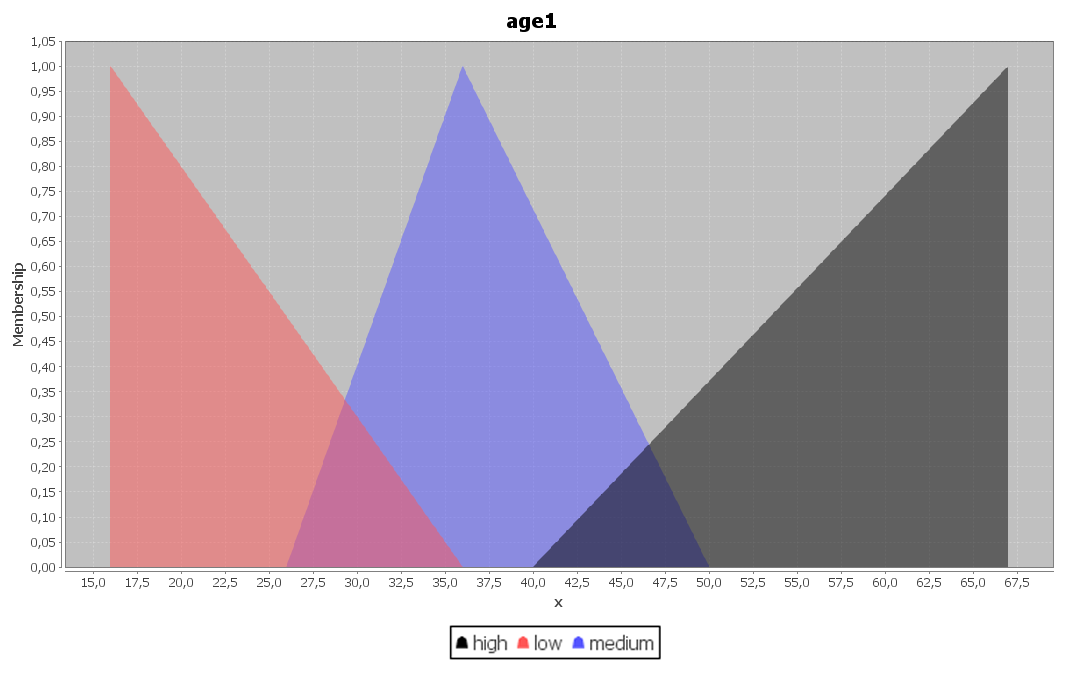
\includegraphics[width=0.9\linewidth]{4_fuzzy-sets-age}
		\caption[Age fuzzy sets]{Age fuzzy sets}
		\label{fig:fs-age}
	\end{figure}

\item \textbf{Experience1}, \textbf{Experience2}. Individual user work experience, whose levels are depicted in Figure \ref{fig:fs-exp}.
\end{itemize}

	\begin{figure}
		\centering
		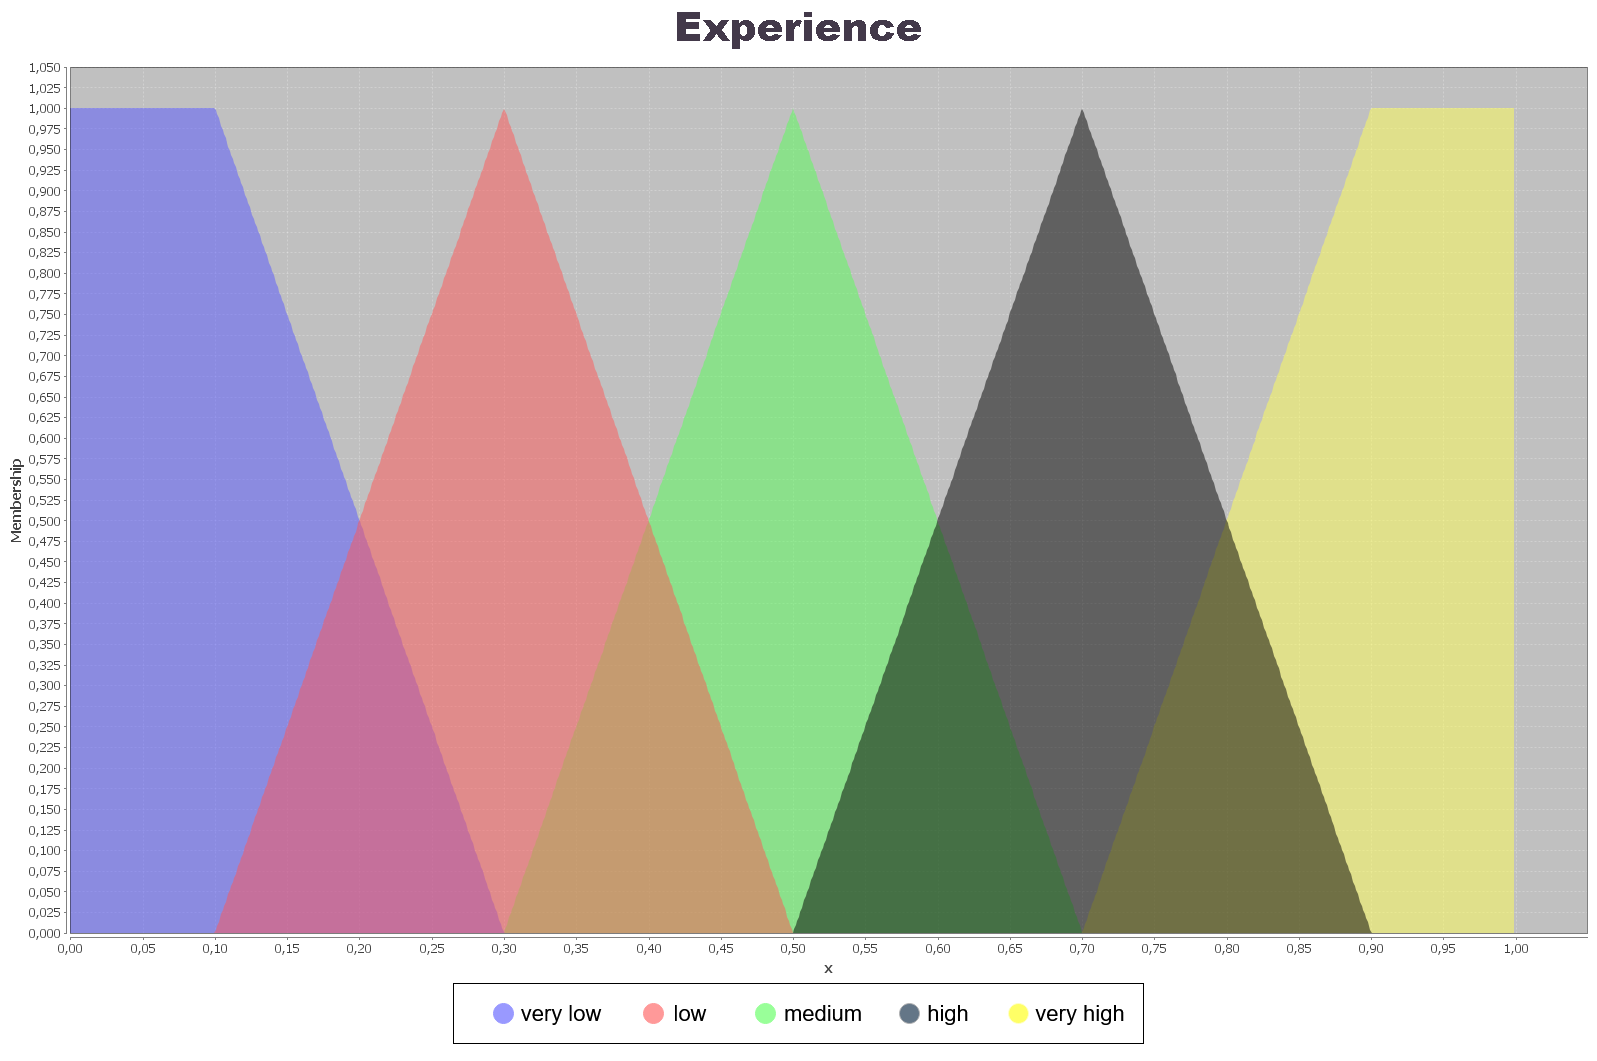
\includegraphics[width=0.9\linewidth]{4_fuzzy-sets-experience}
		\caption[Experience fuzzy sets]{Experience fuzzy sets}
		\label{fig:fs-exp}
	\end{figure}

\indent \textbf{b) Output variables}

\begin{itemize}
\item \textbf{Mediator}. Indicates whether a mediator is needed if there is a high cultural distance between users. It is a singleton set with singleton centre of gravity (COGS) as defuzzification method, as shown in Figure \ref{fig:fs-mediator}.

	\begin{figure}
		\centering
		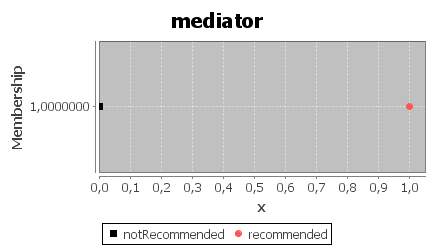
\includegraphics[width=0.6\linewidth]{4_fuzzy-sets-mediator}
		\caption[Mediator singleton fuzzy sets]{Mediator singleton fuzzy sets}
		\label{fig:fs-mediator}
	\end{figure}

\item \textbf{Training}. Represents the need for cultural training when the cultural distance between individuals is medium or moderate. This is another singleton set (see Figure \ref{fig:fs-train}) with COGS as a defuzzification method.

	\begin{figure}
		\centering
		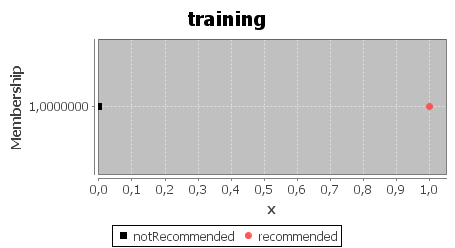
\includegraphics[width=0.6\linewidth]{4_fuzzy-sets-training}
		\caption[Training singleton fuzzy sets]{Training singleton fuzzy sets}
		\label{fig:fs-train}
	\end{figure}

\item \textbf{Supervisor1}, \textbf{Supervisor2}. They represent the need for supervisors for inexperienced users. This need is represented by singleton sets and COGS as defuzzification method (see Figure \ref{fig:fs-super}).

	\begin{figure}
		\centering
		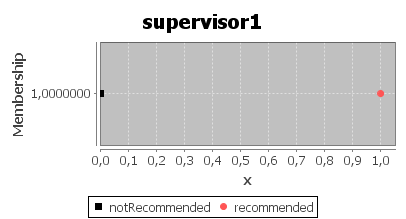
\includegraphics[width=0.6\linewidth]{4_fuzzy-sets-supervisor}
		\caption[Supervisor singleton fuzzy sets]{Supervisor singleton fuzzy sets}
		\label{fig:fs-super}
	\end{figure}

\item \textbf{Solution1}, \textbf{Solution2}, …, \textbf{Solution9}. These variables cover the 9 solutions proposed to reduce communication problems. Each solution shows a series of recommendations and communication means related to user input values. All of them are represented by singleton sets with COGS as defuzzification method (see Figure \ref{fig:fs-solution}). Also note how the proposed communication solution offered as output will be always unique. 
\end{itemize}

	\begin{figure}
		\centering
		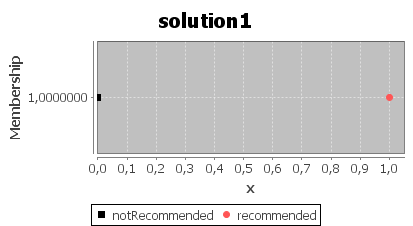
\includegraphics[width=0.6\linewidth]{4_fuzzy-sets-solution}
		\caption[Solutions singleton fuzzy sets]{Solutions singleton fuzzy sets}
		\label{fig:fs-solution}
	\end{figure}

With the input and output variables defined, using jFuzzyLogic for the implementation was not difficult after learning how to use it together with FCL. In general, the system is divided into four distinct parts:

\begin{itemize}
\item First, we have the variable declaration block, as shown in Listing \ref{lst:variables}, where we indicate the input and output variables of the system.

\begin{lstlisting}[caption={[Variables declaration]Variables declaration}, label=lst:variables]
VAR_INPUT
	culturalDist : REAL;
	overlap : REAL;
	age1 : REAL;
	age2 : REAL;
	englishLevel : REAL;
	experience1 : REAL;
	experience2 : REAL;
END_VAR

VAR_OUTPUT
	mediator : REAL;
	training : REAL;
	supervisor1 : REAL;
	supervisor2 : REAL;
	solution1 : REAL;
	solution2 : REAL;
	solution3 : REAL;
	solution4 : REAL;
	solution5 : REAL;
	solution6 : REAL;
	solution7 : REAL;
	solution8 : REAL;
	solution9 : REAL;
END_VAR
\end{lstlisting}

\item Next is the definition block for fuzzy sets, or fuzzification block, where the input values are translated into fuzzy labels (Listing \ref{lst:fuzzification}).

\begin{lstlisting}[caption={[Fuzzification block]Fuzzification block}, label=lst:fuzzification]
FUZZIFY culturalDist // Cultural distance
	TERM veryLow := trape 0 0 0.1 0.3;
	TERM low := trian 0.1 0.3 0.5;
	TERM medium := trian 0.3 0.5 0.7;
	TERM high := trian 0.5 0.7 0.9;
	TERM veryHigh := trape 0.7 0.9 1 1;
END_FUZZIFY

FUZZIFY overlap // Time overlap
	TERM veryLow := trape 0 0 0.1 0.3;
	TERM low := trian 0.1 0.3 0.5;
	TERM medium := trian 0.3 0.5 0.7;
	TERM high := trian 0.5 0.7 0.9;
	TERM veryHigh := trape 0.7 0.9 1 1;
END_FUZZIFY

FUZZIFY age1 // User1's age
	TERM low := trian 16 16 36;
	TERM medium := trian 26 36 50;
	TERM high := trian 40 67 67;
END_FUZZIFY

FUZZIFY age2 // User2's age
	TERM low := trian 16 16 36;
	TERM medium := trian 26 36 50;
	TERM high := trian 40 67 67;
END_FUZZIFY

FUZZIFY englishLevel // English level
	TERM veryLow := trape 0 0 0.1 0.3;
	TERM low := trian 0.1 0.3 0.5;
	TERM medium := trian 0.3 0.5 0.7;
	TERM high := trian 0.5 0.7 0.9;
	TERM veryHigh := trape 0.7 0.9 1 1;
END_FUZZIFY

FUZZIFY experience1 // Experience of user1
	TERM veryLow := trape 0 0 0.1 0.3;
	TERM low := trian 0.1 0.3 0.5;
	TERM medium := trian 0.3 0.5 0.7;
	TERM high := trian 0.5 0.7 0.9;
	TERM veryHigh := trape 0.7 0.9 1 1;
END_FUZZIFY

FUZZIFY experience2 // Experience of user2
	TERM veryLow := trape 0 0 0.1 0.3;
	TERM low := trian 0.1 0.3 0.5;
	TERM medium := trian 0.3 0.5 0.7;
	TERM high := trian 0.5 0.7 0.9;
	TERM veryHigh := trape 0.7 0.9 1 1;
END_FUZZIFY
\end{lstlisting}

\vspace{16px}
\item In the same way, the output values are defined in the defuzzification block (Listing \ref{lst:defuzzification}), following an inverse process to the preceding one.
\newpage
\begin{lstlisting}[caption={[Defuzzification block]Defuzzification block}, label=lst:defuzzification]
DEFUZZIFY mediator // Communication mediator
	TERM notRecommended := 0;
	TERM recommended := 1;
	METHOD : COGS;
	DEFAULT := 0;
END_DEFUZZIFY

DEFUZZIFY training // Communication training
	TERM notRecommended := 0;
	TERM recommended := 1;
	METHOD : COGS;
	DEFAULT := 0;
END_DEFUZZIFY

DEFUZZIFY supervisor1 // Supervisor for user1
	TERM notRecommended := 0;
	TERM recommended := 1;
	METHOD : COGS;
	DEFAULT := 0;
END_DEFUZZIFY

DEFUZZIFY supervisor2 // Supervisor for user2
	TERM notRecommended := 0;
	TERM recommended := 1;
	METHOD : COGS;
	DEFAULT := 0;
END_DEFUZZIFY

DEFUZZIFY solution1
	TERM notRecommended := 0;
	TERM recommended := 1;
	METHOD : COGS;
	DEFAULT := 0;
END_DEFUZZIFY

DEFUZZIFY solution2
	TERM notRecommended := 0;
	TERM recommended := 1;
	METHOD : COGS;
	DEFAULT := 0;
END_DEFUZZIFY

DEFUZZIFY solution3
	TERM notRecommended := 0;
	TERM recommended := 1;
	METHOD : COGS;
	DEFAULT := 0;
END_DEFUZZIFY

DEFUZZIFY solution4
	TERM notRecommended := 0;
	TERM recommended := 1;
	METHOD : COGS;
	DEFAULT := 0;
END_DEFUZZIFY

DEFUZZIFY solution5
	TERM notRecommended := 0;
	TERM recommended := 1;
	METHOD : COGS;
	DEFAULT := 0;
END_DEFUZZIFY

DEFUZZIFY solution6
	TERM notRecommended := 0;
	TERM recommended := 1;
	METHOD : COGS;
	DEFAULT := 0;
END_DEFUZZIFY

DEFUZZIFY solution7
	TERM notRecommended := 0;
	TERM recommended := 1;
	METHOD : COGS;
	DEFAULT := 0;
END_DEFUZZIFY

DEFUZZIFY solution8
	TERM notRecommended := 0;
	TERM recommended := 1;
	METHOD : COGS;
	DEFAULT := 0;
END_DEFUZZIFY

DEFUZZIFY solution9
	TERM notRecommended := 0;
	TERM recommended := 1;
	METHOD : COGS;
	DEFAULT := 0;
END_DEFUZZIFY
\end{lstlisting}

\vspace{16px}
\item As we have already defined the input and output variables, as well as the fuzzification and defuzzification functions, all that remains is to display the set of rules used by the system, shown in Table \ref{tb:recommender-rules}.

\begin{table}[htb]
	\centering
	\caption{Recommender system rules set}
	\label{tb:recommender-rules}
	\resizebox{\textwidth}{!}{%
	\begin{tabular}{|c|l|}
	\hline
	\textbf{N} &
	  \multicolumn{1}{c|}{\textbf{FCL RULE}} \\ \hline\hline
	1 &
	  \begin{tabular}[c]{@{}l@{}}IF (age1 IS   high OR age2 IS high) AND (overlap IS low OR overlap IS veryLow)  \\ AND  (englishLevel is low OR englishLevel is veryLow) THEN solution1 IS   recommended;\end{tabular} \\ \hline
	2 &
	  \begin{tabular}[c]{@{}l@{}}IF (age1 IS   high OR age2 IS high) AND (overlap IS low OR overlap IS veryLow)\\ AND   (englishLevel is medium) THEN solution2 IS recommended;\end{tabular} \\ \hline
	3 &
	  \begin{tabular}[c]{@{}l@{}}IF (age1 IS   high OR age2 IS high) AND (overlap IS low OR overlap IS veryLow)\\ AND   (englishLevel is high OR englishLevel is veryHigh) THEN solution3 IS   recommended;\end{tabular} \\ \hline
	4 &
	  \begin{tabular}[c]{@{}l@{}}IF (age1 IS   high OR age2 IS high) AND (overlap IS medium OR overlap IS high OR overlap is   veryHigh)\\ AND (englishLevel IS veryHigh OR englishLevel IS high OR   englishLevel IS medium) THEN solution4 IS recommended;\end{tabular} \\ \hline
	5 &
	  \begin{tabular}[c]{@{}l@{}}IF (age1 IS   high OR age2 IS high) AND (overlap IS medium OR overlap IS high OR overlap is   veryHigh)\\ AND (englishLevel IS veryLow OR englishLevel IS low) THEN solution5   IS recommended;\end{tabular} \\ \hline
	6 &
	  \begin{tabular}[c]{@{}l@{}}IF (age1 IS   low OR age1 IS medium) AND (age2 IS low OR age2 IS medium)\\ AND (overlap IS   low OR overlap IS veryLow) AND (englishLevel IS medium OR englishLevel IS   high OR englishLevel IS veryHigh) \\ THEN solution6 IS recommended;\end{tabular} \\ \hline
	7 &
	  \begin{tabular}[c]{@{}l@{}}IF (age1 IS   low OR age1 IS medium) AND (age2 IS low OR age2 IS medium)\\ AND (overlap IS   low OR overlap IS veryLow) AND (englishLevel IS low OR englishLevel IS   veryLow) \\ THEN solution7 IS recommended;\end{tabular} \\ \hline
	8 &
	  \begin{tabular}[c]{@{}l@{}}IF (age1 IS   low OR age1 IS medium) AND (age2 IS low OR age2 IS medium)\\ AND (overlap IS   medium OR overlap IS high OR overlap IS veryHigh)\\ AND (englishLevel IS   veryHigh OR englishLevel IS high OR englishLevel IS medium) THEN solution8 IS   recommended;\end{tabular} \\ \hline
	9 &
	  \begin{tabular}[c]{@{}l@{}}IF (age1 IS   low OR age1 IS medium) AND (age2 IS low OR age2 IS medium) \\ AND (overlap IS   medium OR overlap IS high OR overlap IS veryHigh)\\ AND (englishLevel IS   veryLow OR englishLevel IS low) THEN solution9 IS recommended;\end{tabular} \\ \hline
	10 &
	  IF   (culturalDist IS veryHigh) THEN mediator IS recommended; \\ \hline
	11 &
	  IF   (culturalDist IS high) THEN training IS recommended; \\ \hline
	12 &
	  IF   (experience1 IS low OR experience1 IS veryLow) THEN supervisor1 IS   recommended; \\ \hline
	13 &
	  IF (experience2   IS low OR experience2 IS veryLow) THEN supervisor2 IS recommended; \\ \hline
	\end{tabular}%
	}
\end{table}	

\end{itemize}

\newpage
Once the system was implemented and ready to be used, it was integrated into the FENCE interface.

\subsubsection{EXPERT SYSTEM INTERFACE}

The integration of the expert system with the FENCE interface is quite simple and easy to use. When the user accesses the "Recommendations" window (shown in Figure \ref{fig:recommendations}, the first thing that will be loaded will be the last recommendations generated for the project selected in the dropdown menu. However, if the user wants to recalculate these recommendations to get an up-to-date list, then simply pressing the "Update" button will display the new list of advices.

	\begin{figure}
		\centering
		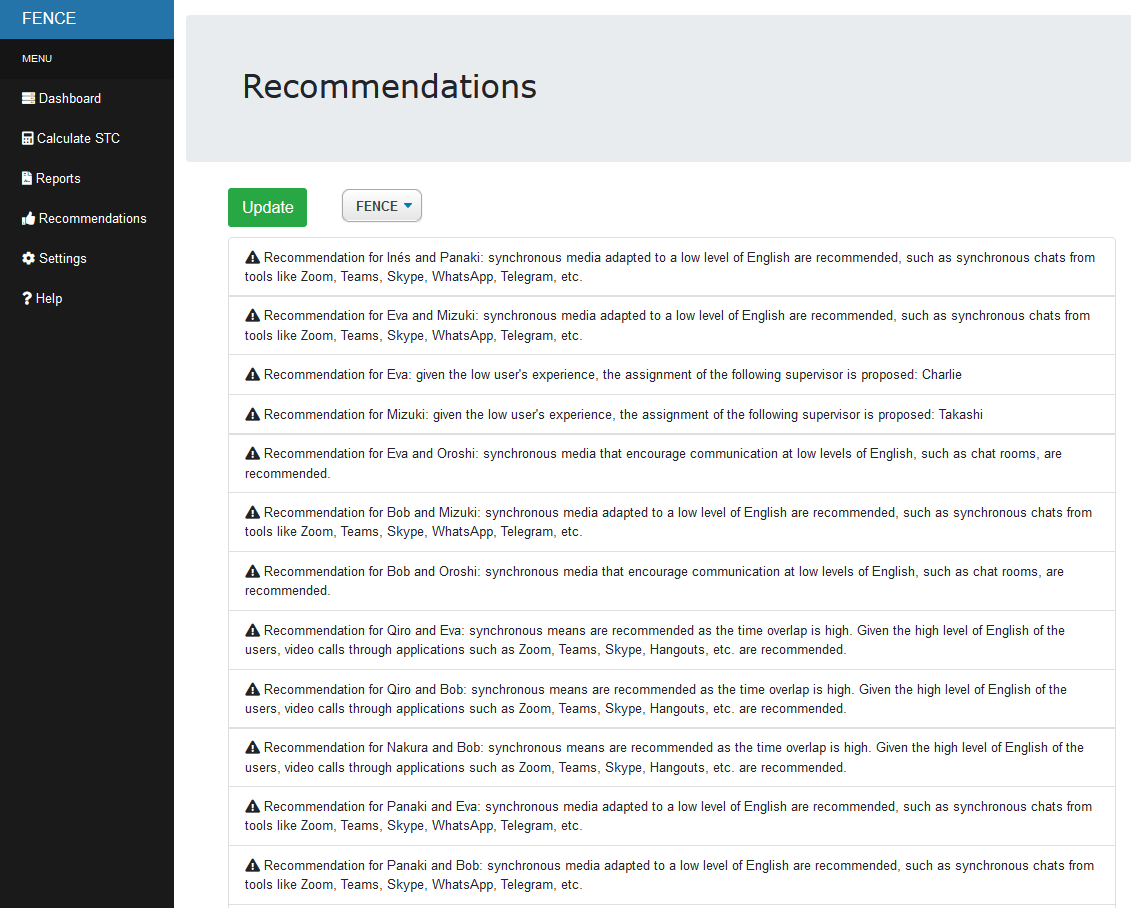
\includegraphics[width=0.9\linewidth]{4_recommendations-window}
		\caption[Recommendations window]{Recommendations window}
		\label{fig:recommendations}
	\end{figure}

As indicated at the beginning of this section, whether or not to show recommendations for certain users should depend on the weight of the coordination gap present among them in the CG matrix. On this basis, one of the improvements proposed at the end of this phase was the possibility of customizing from which weight in CG the system would show recommendations for pairs of employees. This feature as well as others related to customization will be covered in the following section.

\subsection{Module 6. Settings and preferences}

The last functional module of FENCE is the one related to customization and settings. The objectives of this module include enabling the user to modify certain parameters used by the tool so that it can be adjusted to particular projects, teams or user’s needs.

After the development of the STC measurement and recommendation modules, it was agreed that the following customisable features may be implemented:

\begin{itemize}
\item On the one hand, the possibility to generally adjust the weight in the CG matrix considered to provide recommendations between pairs of users. As already explained, when offering recommendations by the expert system, the weight of the cells in CG matrix is taken as a reference to evaluate if there are communication problems between users and, therefore, to know if it is necessary to recommend communication solutions.
\item On the other hand, it was also considered the possibility of establishing custom thresholds for the CG weights used to provide recommendations among specific employees. To better illustrate the customization of this CG weight threshold, let us consider the following example:\newline


\indent\emph{Suppose that the system provides recommendations for any pair of users with a weight in the CG matrix equal to or greater than 0.4.\newline}

\indent\emph{Two users, Alice and Bob, have a lack of coordination reflected in the CG matrix with a value of 0.6, which means that the expert system will offer recommendations to improve their communication.\newline}

\indent\emph{However, we know that the communication between Alice and Bob is simple and effective because they are used to working together, so it would be convenient to be able to adjust the CG threshold value to avoid getting unnecessary recommendations, for example, to 0.9.\newline}

\indent\emph{Thus, the user can set the minimum weight required to receive recommendations for the particular case of Alice and Bob to 0.9 through the FENCE settings interface.\newline}


\end{itemize}

With these ideas in mind, the development of these customizations was conducted (see Figure \ref{fig:settings}. In turn, the option to restore all weights to the established default value was also included, as well as the possibility of establishing these weights at project level, thus increasing customization and flexibility.
\begin{figure}
	\centering
	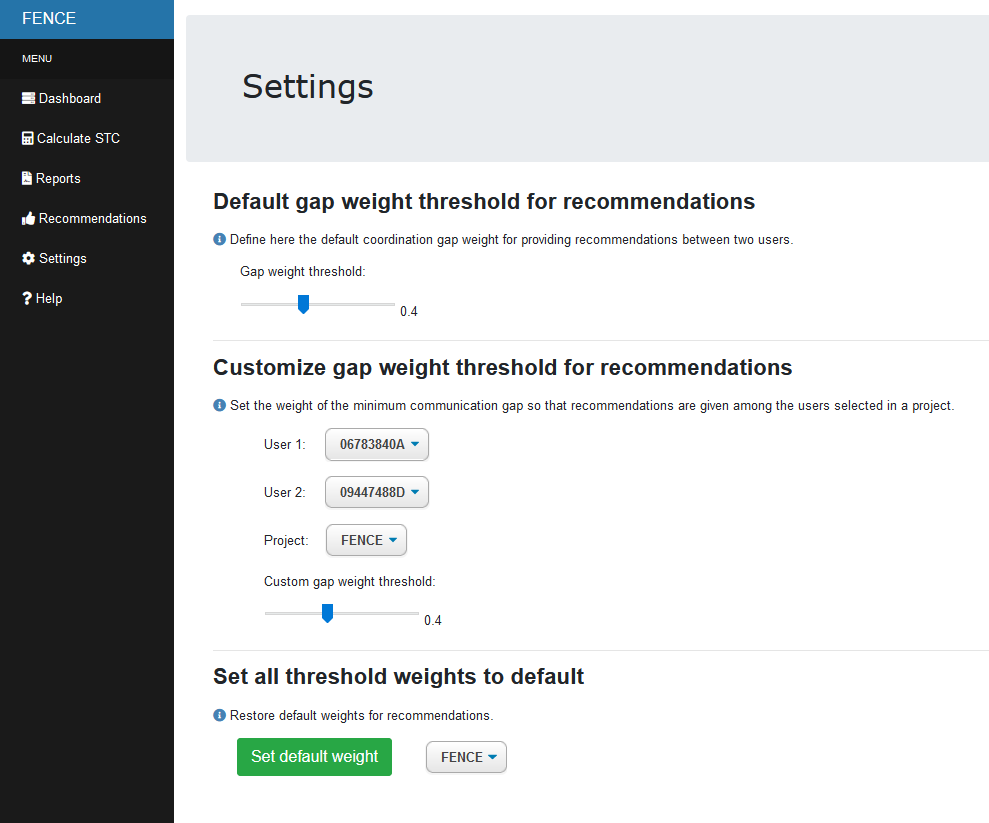
\includegraphics[width=0.9\linewidth]{4_settings-window}
	\caption[Settings window]{Settings window}
	\label{fig:settings}
\end{figure}
In this way, the main functionalities of FENCE had finally been completed. All that remained to be done was to test and make improvements in the presentation and performance of FENCE, an iterative procedure based on stakeholders' feedback.

\section{Transition phase}

Although the tool was already functional and ready to be used, there were still some non-functional changes and actions to be performed. This transition stage includes the performance, usability and optimization testing of FENCE, as well as the deployment of the tool. This actions will be explained in the following subsections.

\subsection{Interface improvements}

With the backend part completed, efforts were focused on improving the application's interface and usability. This work involved reorganizing and improving the cascade style sheets (CSS), optimizing the JavaScript code and improving the overall appearance by modifying the HTML views.

Further graphic information, such as icons and coloured buttons, was also included, as well as a “Help” tab with information about STC and the use of FENCE for its proper management.

\subsection{Algorithms optimization and bug resolution}

Bugs related to the expert system and the recommendations provided were resolved, as well as attempts were made to further optimize the STC measurement algorithms.

Moreover, security improved were attempted to be added in order to increase the robustness of the tool, such as input control in the database. However, given the time constraints of the project, this aspect was not addressed as deeply as would have been desired, so it is proposed as a future improvement of the tool.

\subsection{First release and documentation}

Once the tool was finally considered to be completed, the building and packaging of the distributable executable of FENCE was performed. At the same time, most of the tool's documentation was produced in this phase: both in the GitHub repository where it is hosted and in this document itself.

\subsection{Application deployment}

Finally, the application was deployed on the Heroku cloud platform. This platform as a service (PaaS) allows free and limited deployment of cloud services, serving as an example of how FENCE would be used in a real web environment (see Figure \ref{fig:heroku-app}, where the service hosted on \url{www.fenceapp.herokuapp.com} is shown).
	
	\begin{figure}
		\centering
		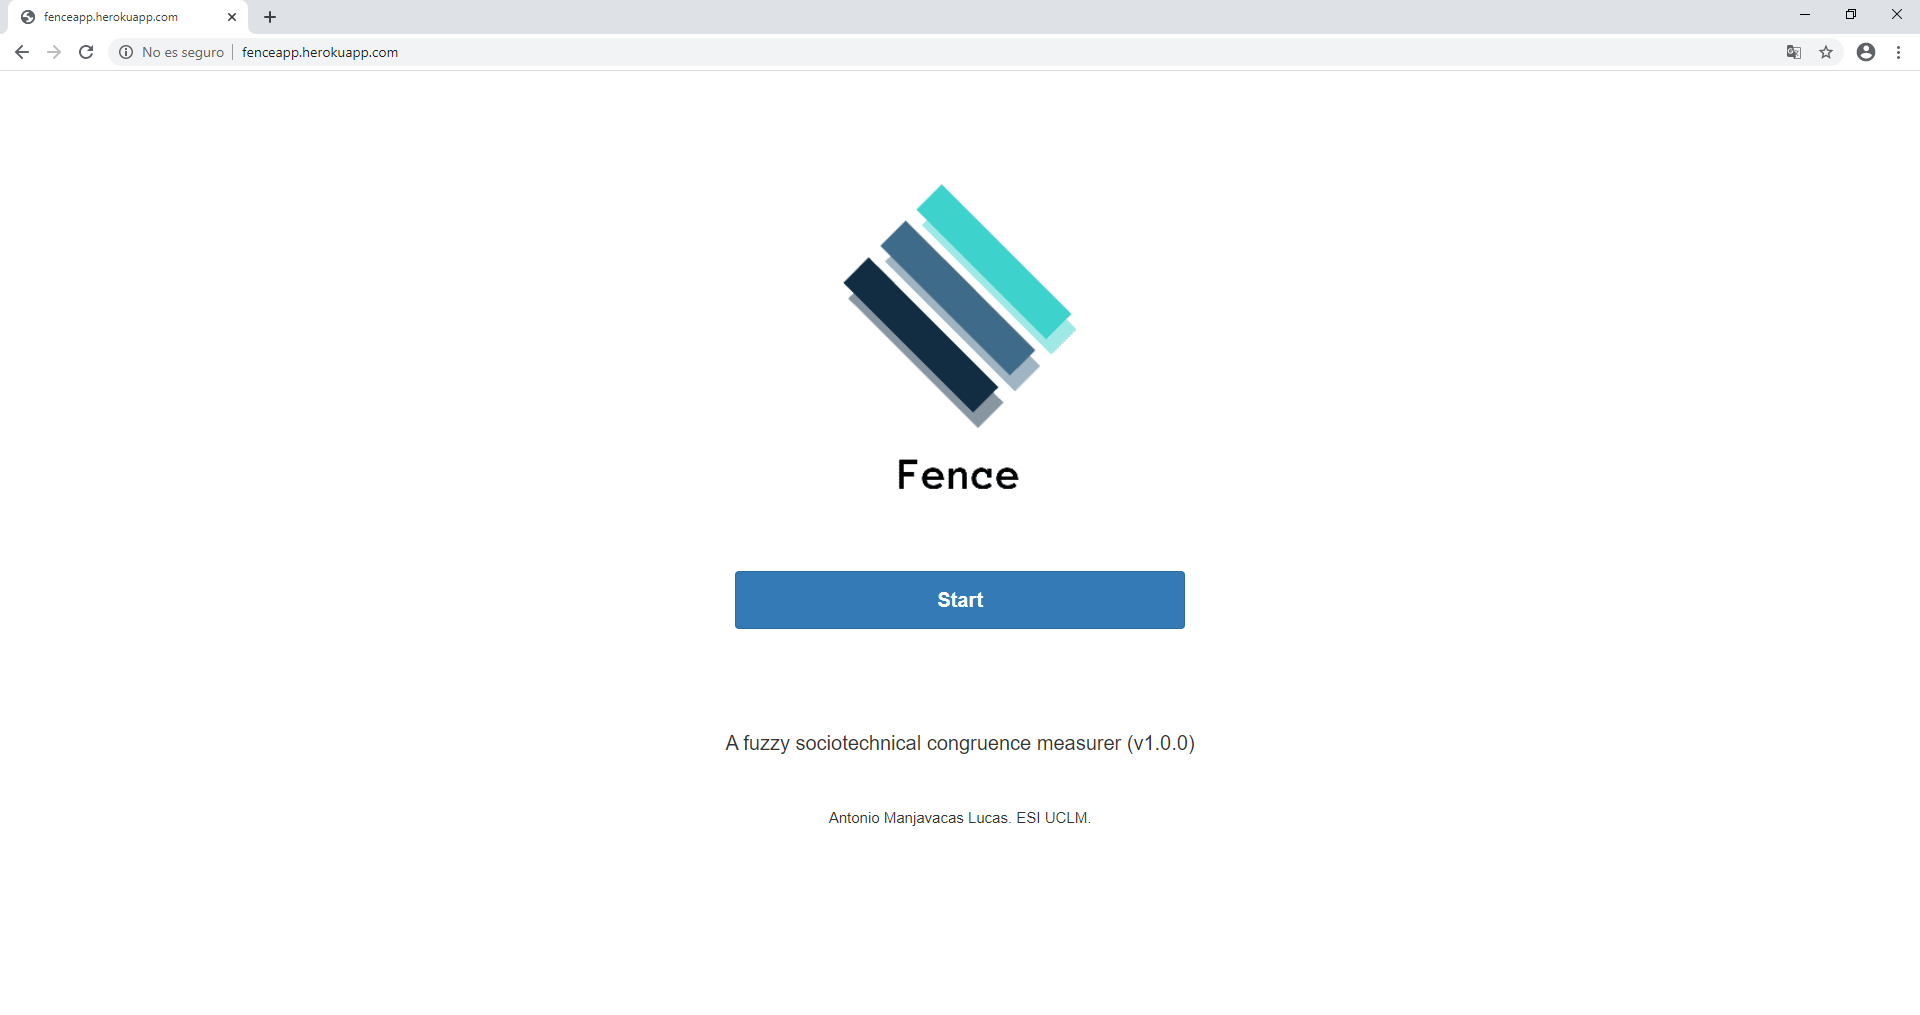
\includegraphics[width=0.9\linewidth]{4_heroku-app}
		\caption[FENCE deployed in Heroku]{FENCE deployed in Heroku Cloud Platform}
		\label{fig:heroku-app}
	\end{figure}

It should also be noted that FENCE was initially considered as a tool for local use, and that it would be necessary to include security and access policies to ensure its concurrent use by multiple users. However, it can be seen that in this first version it is completely operative on the web, and that it would be a matter of future improvements to better adapt the tool to a fully distributed environment.
\chapter{Conclusions}
\label{cap:conclusions}

In this last chapter, we shall address the conclusions to which the project has led. We shall first look at how the project objectives have been met and how the project has been justified with the intensification competencies. We shall subsequently discuss future work and personal assessments after the completion of the project.

\section{Achievement of the objectives}

The general objectives established at the beginning of this project were: the development of a tool with which to measure STC within an organisation, along with a recommendation system that could be used to improve the organisation's STC levels.

At this point, we can confirm the fulfilment of both objectives and we shall now, therefore, provide details on how they have been achieved by meeting the different specific objectives of the project:

\begin{itemize}
\item The project began with the development of a dashboard with which to allow the manipulation of the resources required in order to measure STC in an organisation. This was a challenging functional module, as it required training in frontend resources that the student had never previously used. Time constraints prevented the control of inputs and outputs, along with more robust testing, from being carried out to the level desired. Despite this, the functional module fulfils its task and meets the requirements of the tool without major problems.\newline

\item The subsequent implementation of the algorithms required in order to measure STC and its adaptation to GSD was undoubtedly the functionality that required the greatest amount of time. Efforts were also made to attempt to improve their performance and refine the measurement by means of a fuzzy inference system. This objective also involved the simulation of communications in order to test the algorithms, the interface corresponding to this functional module and consultations with an expert in order to refine the measurements.\newline

\item One of the principal contributions of FENCE is the use of a fuzzy inference system to improve STC measurement. Working with attributes expressed through linguistic labels provided the possibility of using a fuzzy inference system to improve the calculation of STC levels. This functionality can also be considered as an original contribution if we compare it with other existing tools used to measure STC \cite{sierra_systematic_2018}, since it allows the system to be more flexible for organizations with different socio-cultural distances that can impact on STC levels.\newline

\item In comparison with the previous modules, the visualization of the STC history levels meant less effort than expected, since the main tasks carried out were training in the use of \emph{Chart.js} and the adaptation of the data model to the needs of the timelines. The greatest difficulty was, again, the use of frontend technologies not previously employed, although in this case it was not a major challenge.\newline

\item Finally, the implementation of the recommendation system for the improvement of STC levels was another of the most challenging milestones of the project. The complexity of this functional module meant exploring the processes of Knowledge Engineering and fuzzy logic in greater depth. It was also necessary to study the FCL standard and the jFuzzyLogic library in order to translate the expert knowledge into rules that could be used by the system. It is worth noting that one of the features that emerged while developing the expert system was the customization of threshold weights with which to provide recommendations. This feature, which was not originally intended, was added with the intention of improving the recommendations offered and making FENCE a more flexible tool.

\end{itemize}

As can be seen, the objectives set out at the beginning of the project were achieved. Furthermore, some of them were even expanded in order to improve the tool with features not initially contemplated, and this highlighted the importance of continuous communication with stakeholders throughout the project.

\section{Competencies justification}

This section provides the rationale for the Computation competencies addressed in this project. Let us, therefore, study the competencies covered during the development of FENCE:

\begin{description}
\item[CM3:]\emph{Ability to evaluate the computational complexity of a problem, discover algorithmic strategies that can lead to its resolution and recommend, develop, and implement that which guarantees the best performance according to requirements}.\newline  

	This project has led to a detailed study and more profound exploration of algorithms already existing in literature, with the objective of measuring STC. The existing algorithms were simultaneously improved and adapted to the specific needs of GSD contexts.\newline

\item[CM4:]\emph{Ability to understand the fundamentals, paradigms, and techniques of intelligent systems and to analyse, design and build computer systems, services and applications using these techniques in any field of application}.\newline 

	The development of FENCE has involved the implementation of an intelligent system for the measurement and improvement of STC. Fuzzy inference systems have been specifically used to achieve this goal.\newline

\item[CM5:]\emph{Ability to acquire, obtain, formalize, and represent human knowledge in a computable manner for problem solving by means of a computer system in any field of application, particularly those related to aspects of computing, perception and performance in environments or intelligent environments}.\newline 

	This competence has been addressed through the development of a knowledge-based system.  Its implementation has involved Knowledge Engineering procedures, in addition to the formalization and representation of knowledge through the use of fuzzy rules.

\end{description}

\section{Lessons learned}

The development of this project has made it possible to relate the importance of STC in organisations, its significant influence in GSD contexts and how useful it is to employ fuzzy logic and knowledge-based systems in order to improve it.

With regard to the STC measurement, various alternatives were initially studied when deciding which algorithms to use for FENCE. The STC measurement method outlined by Cataldo et al. \cite{cataldo_identification_2006, cataldo_socio-technical_2008} was discarded owing to the low flexibility provided by its bivalued-weight matrices. Other metrics, such as that of Valetto et al. \cite{valetto_using_2007} could not be adapted to GSD contexts, as explained in \cite{sierra_systematic_2018}. Only the solutions proposed by Portillo et al. \cite{portillo_2014} and Kwan et al. \cite{kwan_weighted_2009, kwan_does_2011} were suitable for such environments, being the proposal of Kwan et al. the one finally chosen, since it is a more general procedure and, therefore, more open and adaptable to FENCE requirements.

It was simultaneously necessary to carry out a reformulation of the algorithms presented by Kwan et al. in order to improve their performance as much as possible. This was achieved by replacing the use of matrices with objects stored in the database, thus reducing their complexity and, therefore, execution time.

Furthermore, extracting expert knowledge was not an easy task and it took several meetings to agree on a robust proposal that would serve as the basis for the expert system. The development of this expert system signified the need to make major efforts with the knowledge engineer such as in-depth individual research into unknown topics in order to better extract expert knowledge; the planning of structured interviews that would guarantee the expert's comfort when contributing expertise, or dealing with the ambiguity of human language.

One of the most valuable lessons learned from this project was that going into greater depth throughout its development could lead to the consideration of improvements not initially contemplated but which provided the tool with significant value. As an example, in the early days of FENCE, we did not contemplate the customisation of threshold weights in order to provide recommendations, but after a discussion we agreed that it could be an interesting feature to be added. Any changes agreed with stakeholders that do not involve a major departure from the main objectives of the project should, therefore, be welcomed as long as they add value and are profitable.

Moreover, it is important to emphasize the relevance of carrying out a detailed study of the tools that are being used. It took several days to compare multiple Java fuzzy logic libraries and, once chosen, the development of the fuzzy inference systems required training time, not only as regards the libraries used in the papers published by their authors, but also as regards the notions of fuzzy logic. This was necessary work that took several weeks, although the time invested was worthwhile and speeded up the process of implementing the system.

In this development, it was also necessary to learn the basic syntax of FCL (structures, variables, functions, etc.). This resulted in a really useful and interesting fuzzy control language, which the author recommends when confronting projects based on fuzzy inference systems.

The development of FENCE using tools such as Spring Boot, HTML, JavaScript, CSS or jQuery together for the first time was also a real challenge, involving a long period of self-teaching and improvement throughout the project.

Finally, planning was essential. Many of the proposed objectives would not have been easily achieved without the proper management of the time invested in each iteration, anticipating possible problems, reducing risks, and always consulting with stakeholders before advancing on important aspects of the project.

\section{Future work}

Concerning the future work that could be derived from this project, many possibilities can be explored.

First, one of the drawbacks of the algorithms needed to measure STC is their low scalability. Their performance is not sufficiently high when input data (users, tasks, teams, assignments, dependencies) grow to more realistic sizes. In fact, improving the performance of these algorithms is a complex task that we intend to confront as further work. As an example, and considering the matrixial nature of these algorithms, an initial proposal that could be addressed is that of increasing parallelization by means of threads.

Focusing on the recommendation of solutions by which to improve STC, the work presented in this project could be the basis of a much more complex system, providing a greater number of solutions that are not only related to communication. In-depth information concerning dependencies, the availability of different employees, or task deadlines are some of the initial proposals that are suggested as improvements to be addressed in the future.

Moreover, if we focus on the use of data to manage STC, one possible future approach could be the implementation of a functional module that would allow the estimation of future STC levels based on historical measurements and the organisation’s current status.

In conclusion, the possibilities of STC are still wide and varied. This makes STC a broad field of study, in which all the proposed solutions should always lead to the benefit of the organisations and those who shape them.

\section{Personal appraisal}

With regard to personally appraising this project, I consider FENCE to be merely the first step in providing a new approach as to how STC can be measured and improved. My view is that it is a particularly useful and valuable tool if it is put to good use, as it is first and foremost capable of raising the awareness of such important human aspects as coordination and communication.

This project has meant many things to me at a personal level. On the one hand, being able to put into practice what I have learnt during all these years has been a considerable source of motivation and pride. On the other, being able to build bridges between my passion for artificial intelligence and research has also been a tremendous stimulus for me.

Moreover, the development of this project has meant perseverance, self-demand, discipline and, above all, creativity, values that I hope to continue improving over time. This work has undoubtedly also allowed me to look at things in perspective and see how, thanks to these principles, I have arrived where I am today.

Thus, after four years of intense work, this period comes to an end. With no interest in stating more than necessary, the completion of this project closes one of the most important periods of my life, which has modelled me as a person and future engineer and which, despite the enormous efforts and sacrifices it has required, has undoubtedly been worthwhile.

\makeatletter		
\begin{flushright}
	\vspace{1,5cm}
	\textit{\@autor}\\
	Campo de Criptana, June 3rd, 2020.
\end{flushright}
\makeatother
% -------------------------


%--- BACKMATTER
%\backmatter (se comenta para que los índices puedan aparecer después de la bibliografía)



% -------------------------
%
% BIBLIOGRAFÍA
%
% -------------------------
% OJO: Todas las referencias deben estar citadas en el texto)
% EDITAR: Comentar línea siguiente
%\nocite{*} % INCLUIDO para ver cómo queda, pero comentar en versión final.

\cleardoublepage % OJO: Necesario para ajustar el avance de página
\phantomsection  % OJO: Ojo necesario con hyperref.
\addcontentsline{toc}{chapter}{\bibname} % Añade la bibliografía al Índice de contenidos.
%---
% Opción 1: Bibliografía con todas las fuentes en un apartado.
%---
\printbibliography
%---

%---
% Opción 2: Bibliografía con secciones separadas.
%---
%\printbibheading
%\printbibliography[heading=subbibliography,type=online,title={Fuentes online}]
%\printbibliography[heading=subbibliography,nottype=online,title={Fuentes no online}]
% -------------------------


% -------------------------
%
% OPT.: ANEXOS: Comentar si no se desean incluir.
% Mover si se desea que aparezcan antes de la bibliografía.
%
% -------------------------
\appendix
\portadaAnexos % OPT. Añade una portada para anexos

% Tras este punto los capítulos se numeran con letras.
% Aquí todos los apéndices necesarios
\chapter{Simulated communications}
\label{cap:annexA}

This annex includes the Python code used for the generation of random communications (Listing \ref{lst:pycom}). The simulated communication activities were inserted in the corresponding collection within the MongoDB database. Note how the \href{https://api.mongodb.com/python/current/tutorial.html}{PyMongo} library was used for this purpose.

The attributes generated in a simulated way and that constitute a communication activity are the following:

\begin{itemize}
\item \textbf{user1} and \textbf{user2}: the users involved in the bidirectional communication activity.
\item \textbf{taskRef}: identification of the task addressed in the communication activity.
\item \textbf{source}: random communication channel.
\item \textbf{duration}: time spent on synchronous communications.
\item \textbf{date}: random date and hour between January and May of 2020.
\item \textbf{project}: project within which the communication is framed.
\end{itemize}

For security reasons, part of the URI used to make the connection to MongoDB Atlas has been omitted. Therefore, the result of the execution will be a set of simulated communications as the ones shown in Figure \ref{fig:coms}.

\newpage
\lstinputlisting[language=Python,style=Python-color,caption={Random communications generator},label=lst:pycom]{./code/communications.py}

\begin{figure}
	\centering
	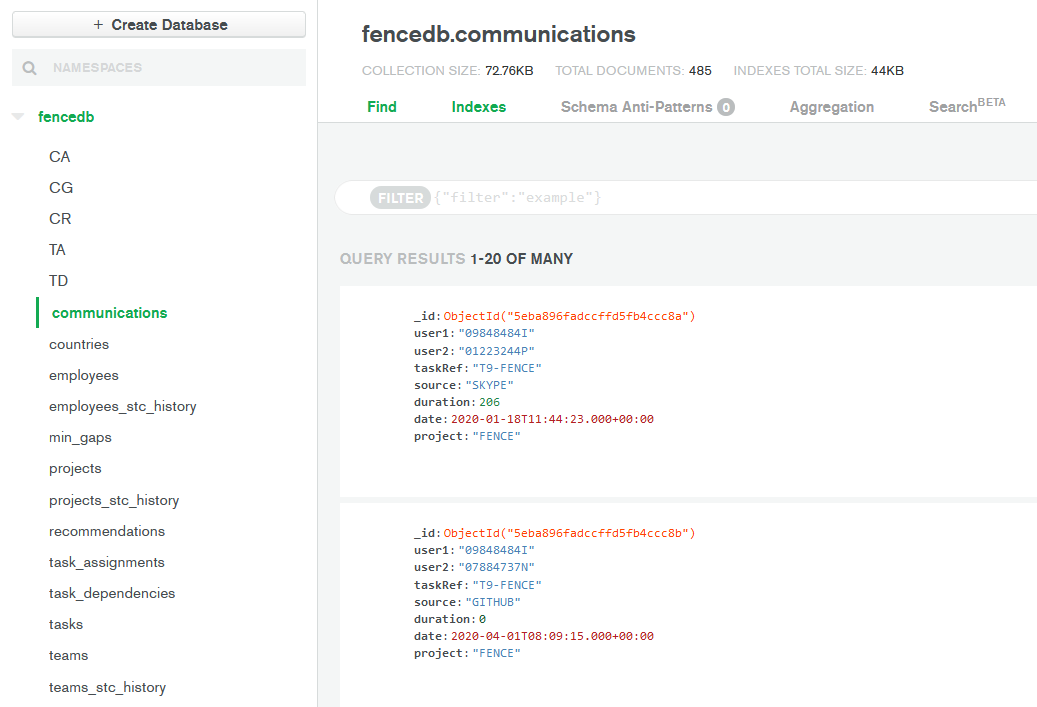
\includegraphics[width=0.95\linewidth]{annex-com}
	\caption[Sample communication activities]{Sample communication activities}
	\label{fig:coms}
\end{figure}

 % Apéndice A (opcionales)
\chapter{Expert system solutions}
\label{cap:annexB}

This appendix details the solutions offered by FENCE's fuzzy recommendation system. These are divided into two groups: on the one hand, the recommendations related to proposed communication strategies (\emph{Solution 1}, \emph{Solution 2}, ..., \emph{Solution 9}), independent of the \emph{Mediator}, \emph{Training} and \emph{Supervisor} solutions, focused on reducing socio-cultural distances or favouring the efforts of less experienced users.

\section{Communication solutions}

\begin{itemize}

\item \textbf{Solution 1}: asynchronous means are recommended given a low time overlap. The communication is adapted to the age of the users and their level of English, proposing as main means of communication e-mail and conventional documentation.\newline

\item \textbf{Solution 2}: asynchronous means are recommended given the low time overlap. Given an average fluency in English, Wikis and e-mail are encouraged as the main means of communication, with the possibility of relying on conventional documentation.\newline

\item \textbf{Solution 3}: asynchronous means adapted to low time overlap are recommended. Given the high level of English of both users, email, chats and Wikis are recommended as the main means of communication, depending on the circumstances.\newline

\item \textbf{Solution 4}: synchronous means are advisable in view of the high time overlap. Given the high level of English of the users, the use of the conventional phone calls is recommended.\newline

\item \textbf{Solution 5}: synchronous media that encourage communication at low levels of English, such as chat rooms, are recommended.\newline

\item \textbf{Solution 6}: asynchronous means are recommended given the low time overlap. As there is a common command of English, corporate chats are recommended as the main means of communication (e.g. Teams or Jira).\newline

\item \textbf{Solution 7}: asynchronous means are recommended to suit the low level of English of the users. Recommended media capable of meeting these requirements are Slack and Github.\newline

\item \textbf{Solution 8}: synchronous means are recommended as the time overlap is high. Given the high level of English of the users, video calls through applications such as Zoom, Teams, Skype, Hangouts, etc. are recommended.\newline

\item \textbf{Solution 9}: synchronous media adapted to a low level of English are recommended, such as synchronous chats from tools like Zoom, Teams, Skype, WhatsApp, Telegram, etc.\newline

\end{itemize}

\section{Other solutions}

\begin{itemize}

\item \textbf{\emph{Mediator} solution}: given the high cultural differences between users, a mediator is recommended to intercede between them in order to ensure proper communication.\newline

\item \textbf{\emph{Training} solution}: socio-cultural training is recommended to reinforce communication between users: manuals, training or any other awareness solution.\newline

\item \textbf{\emph{Supervisor} solution}: given the low user's experience, the assignment of the following supervisor is proposed: ...\newline

\end{itemize} % Apéndice B (opcionales)
%---



% -------------------------
%
% OPT.: ÍNDICE TEMÁTICO: Comentar si no se desean incluir.
%
% -------------------------
% CONSEJO: Incluir los comandos mientras se escribe cada capítulo ya que hacerlo al final resulta tedioso.
%\cleardoublepage % OJO: Necesario para ajustar el avance de página
%\phantomsection  % OJO: Ojo necesario con hyperref.
% EDITAR: Si se desea cambiar el nombre del índice temático
%\renewcommand{\indexname}{Thematic index}
%\addcontentsline{toc}{chapter}{\indexname} % Añade al Índice de contenidos.
%\printindex  % Facilitado por makeidx (opcional, si no se usa no se imprime)
%---
\end{document}